%----------
%   WARNING
%----------

% This Guide contains Library recommendations based mainly on APA and IEEE styles, but you must always follow the guidelines of your TFG Tutor and the TFG regulations for your degree.

% THIS TEMPLATE IS BASED ON THE IEEE STYLE 


%----------
% DOCUMENT SETTINGS
%----------

\documentclass[12pt]{report} % font: 12pt

% margins: 2.5 cm top and bottom; 3 cm left and right
\usepackage[
a4paper,
vmargin=2.5cm,
hmargin=3cm
]{geometry}

% Paragraph Spacing and Line Spacing: Narrow (6 pt / 1.15 spacing) or Moderate (6 pt / 1.5 spacing)
\renewcommand{\baselinestretch}{1.15}
\parskip=6pt

% Color settings for cover and code listings 
\usepackage[table]{xcolor}
\definecolor{azulUC3M}{RGB}{0,0,102}
\definecolor{gray97}{gray}{.97}
\definecolor{gray75}{gray}{.75}
\definecolor{gray45}{gray}{.45}

% PDF/A -- Important for its inclusion in e-Archive. PDF/A is the optimal format for preservation and for the generation of metadata: http://uc3m.libguides.com/ld.php?content_id=31389625. 

% In the template we include the file OUTPUT.XMPDATA. You can download that file and include the metadata that will be incorporated into the PDF file when you compile the memoria.tex file. Then upload it back to your project.  
\usepackage[a-1b]{pdfx}

% LINKS
\usepackage{hyperref}
\hypersetup{colorlinks=true,
	citecolor=black,
	linkcolor=black, % links to parts of the document (e.g. index) in black
	urlcolor=blue} % links to resources outside the document in blue

% MATH EXPRESSIONS
\usepackage{amsmath,amssymb,amsfonts,amsthm}

% Character encoding
\usepackage{txfonts} 
\usepackage[T1]{fontenc}
\usepackage[utf8]{inputenc}

% English settings
\usepackage[english]{babel} 
\usepackage[babel, english=american]{csquotes}
\AtBeginEnvironment{quote}{\small}

% Footer settings
\usepackage{fancyhdr}
\pagestyle{fancy}
\fancyhf{}
\renewcommand{\headrulewidth}{0pt}
\rfoot{\thepage}
\fancypagestyle{plain}{\pagestyle{fancy}}

% DESIGN OF THE TITLES of the parts of the work (chapters and epigraphs or sub-chapters)
\usepackage{titlesec}
\usepackage{titletoc}
\titleformat{\chapter}[block]
{\large\bfseries\filcenter}
{\thechapter.}
{5pt}
{\MakeUppercase}
{}
\titlespacing{\chapter}{0pt}{0pt}{*3}
\titlecontents{chapter}
[0pt]                                               
{}
{\contentsmargin{0pt}\thecontentslabel.\enspace\uppercase}
{\contentsmargin{0pt}\uppercase}                        
{\titlerule*[.7pc]{.}\contentspage}                 

\titleformat{\section}
{\bfseries}
{\thesection.}
{5pt}
{}
\titlecontents{section}
[5pt]                                               
{}
{\contentsmargin{0pt}\thecontentslabel.\enspace}
{\contentsmargin{0pt}}
{\titlerule*[.7pc]{.}\contentspage}

\titleformat{\subsection}
{\normalsize\bfseries}
{\thesubsection.}
{5pt}
{}
\titlecontents{subsection}
[10pt]                                               
{}
{\contentsmargin{0pt}                          
	\thecontentslabel.\enspace}
{\contentsmargin{0pt}}                        
{\titlerule*[.7pc]{.}\contentspage}  


% Tables and figures settings
\usepackage{multirow} % combine cells 
\usepackage{caption} % customize the title of tables and figures
\usepackage{floatrow} % we use this package and its \ ttabbox and \ ffigbox macros to align the table and figure names according to the defined style.
\usepackage{array} % with this package we can define in the following line a new type of column for tables: custom width and centered content
\newcolumntype{P}[1]{>{\centering\arraybackslash}p{#1}}
\DeclareCaptionFormat{upper}{#1#2\uppercase{#3}\par}
\usepackage{graphicx}

% CODE LISTINGS
% support and styling for listings. More information in  https://es.wikibooks.org/wiki/Manual_de_LaTeX/Listados_de_código/Listados_con_listings
\usepackage{listings}

% Custom listing
\lstdefinestyle{estilo}{ frame=Ltb,
	framerule=0pt,
	aboveskip=0.5cm,
	framextopmargin=3pt,
	framexbottommargin=3pt,
	framexleftmargin=0.4cm,
	framesep=0pt,
	rulesep=.4pt,
	backgroundcolor=\color{gray97},
	rulesepcolor=\color{black},
	%
	basicstyle=\ttfamily\footnotesize,
	keywordstyle=\bfseries,
	stringstyle=\ttfamily,
	showstringspaces = false,
	commentstyle=\color{gray45},     
	%
	numbers=left,
	numbersep=15pt,
	numberstyle=\tiny,
	numberfirstline = false,
	breaklines=true,
	xleftmargin=\parindent
}

\captionsetup*[lstlisting]{font=small, labelsep=period}
 
\lstset{style=estilo}
\renewcommand{\lstlistingname}{\uppercase{Código}}


% REFERENCES 

%-------------
%	DOCUMENT
%-------------

\begin{document}
\pagenumbering{roman} % Roman numerals are used in the numbering of the pages preceding the body of the work.

%----------
%	COVER
%----------	
\begin{titlepage}
	\begin{sffamily}
		\color{azulUC3M}
		\begin{center}
			\begin{figure}[H] % UC3M Logo
				\makebox[\textwidth][c]{
\includegraphics[width=10cm]{Figures/template/UWTSD-Logo.png}}
			\end{figure}
			\vspace{2.5cm}
			\begin{Large}
				MSc Degree in Software Engineering and Artificial Intelligence\\
				2022-2023\\ % Academic year
				\vspace{2cm}
				\textsl{MSc Thesis}
				\bigskip

			\end{Large}
			{\Huge ``Enhancing Self-Driving Car Performance: The Potential Dangers of Autonomous Vehicles and Motorcycles''}\\
			\vspace*{0.5cm}
			\rule{10.5cm}{0.1mm}\\
			\vspace*{0.9cm}
			{\LARGE Edward Samuel Ralph Patch}\\
			\vspace*{1cm}
			\begin{Large}
				Dr. Tim Bashford\\
				Waterfront Campus - 2023\\
			\end{Large}
		\end{center}
		\vfill
		\color{black}

	\end{sffamily}
\end{titlepage}

\newpage % blank page
\thispagestyle{empty}
\mbox{}

\newpage % blank page
\thispagestyle{empty}
\mbox{}

%----------
%	ABSTRACT AND KEYWORDS 
%----------	
\renewcommand\abstractname{\large\bfseries\filcenter\uppercase{Summary}}
\begin{abstract}
	\thispagestyle{plain}
	\setcounter{page}{3}

	% Write your abstract
	 This dissertation focuses on the safety development of Autonomous Vehicles and Motorcycles using Artificial Neural Networks. The research question involves, `Are AVs a danger to motorcyclists?' hypothesising the safety aspects of blindspots, poor visibility and poor weather conditions to support the research question. The datasets used a combination of Asian and US road footage. The training performance of the model within the report achieves 81\% accuracy for motorcycles in a filtered Dataset A involving pedestrians and a wide range of vehicles, 77.5\% accuracy in a filtered Dataset B involving motorcycles, trikes and pedestrians, and 61\% accuracy in Dataset C including a simulated night-time version of Dataset A. These training results give an idea of the detection result's accuracy. A precision and recall curve diagram shows the curvature of the learning process to help identify any critical errors in the training process and the model's reliability. The previous research to build this report involved looking into how Autonomous Vehicles, ADAS and V2V communications are currently implemented. This aspect establishes how vehicles currently function and what previous and current technologies are in place. The current findings highlight some dangerous misclassification entries on UK roads, which requires a deeper understanding of enhancing safety infrastructure on Autonomous Vehicles. The hypotheses are covered. Hypothesis A, `Motorcycles have blindspots that are often overlooked by human drivers, which AVs can detect and avoid.' was found to be untrue from the limited research and experimentations conducted in this thesis. Hypothesis B, `In low light conditions, AVs may struggle to accurately detect and identify motorcycles, leading to potential safety issues on the road.' was proven to fall in the factual category, not down to low light conditions such as the model did exceptionally well at detecting the motorcycle, even if the time frame was not in the ideal zones, but more down to light glare from upcoming vehicles. This fact meant that the motorcyclist was hidden, and the object classification could not detect the motorcycle until the glare calmed down. Hypothesis C, `Poor weather conditions, such as heavy rain or poor visibility, can make it difficult for AVs to detect and react to motorcycles, increasing the risk of accidents.' was proven to be authentic as camera glare, water droplets, and spray caused classifications for motorcycles to misidentify, pursuing potential emergency braking when late classification proceeds. Overall, the experiments went better than expected, and the results, establishing the Legal Issues, Motorcycle Safety Training, and AV Methodology, helped identify how these risks are mitigated.

	\textbf{Keywords:} % add the keywords
	Artificial Neural Networks, Autonomous Vehicles, Motorcycle Safety.
	\vfill
\end{abstract}
\newpage % Blank page
\thispagestyle{empty}
\mbox{}
%----------
%	Acknowledgements
%----------	
\chapter*{Acknowledgements}

\setcounter{page}{5}
We extend our deepest gratitude to Kaden Summers and Jonathon Patch, whose invaluable contributions as motorcyclists greatly enriched this project. Their tireless efforts in capturing testing footage from Carmarthenshire to Powys in Wales, under rainy and clear conditions provided critical qualitative data to our research. The visual material they obtained was instrumental in offering a comprehensive understanding of the subject.
	
Special appreciation goes to Jonathon Patch, who participated in the fieldwork and generously provided the camera equipment necessary to record the footage. Their collaboration and unwavering support have played a pivotal role in advancing this research; for that, we are profoundly thankful.	
\vfill

\newpage % blank page
\thispagestyle{empty}
\mbox{}

%-----------
%	Project Details
%-----------
\chapter*{Repository and Project Resources}
\setcounter{page}{6}
	\begin{description}
		\item[Repository:] \href{https://github.com/ShinkuKira21/Autonomous-Vehicles-Motorcycle-Safety}{https://github.com/ShinkuKira21/Autonomous-Vehicles-Motorcycle-Safety}
		\item[Project:] \href{https://github.com/users/ShinkuKira21/projects/2/}{https://github.com/users/ShinkuKira21/projects/2/}
  	\end{description}
\vfill

\newpage % blank page
\thispagestyle{empty}
\mbox{}

%----------
%	TOC
%----------	

%--
% TOC
%-
\tableofcontents
\thispagestyle{fancy}

\newpage % blank page
\thispagestyle{empty}
\mbox{}

%--
% List of figures. If they are not included, comment the following lines
%-
\listoffigures
\thispagestyle{fancy}

\newpage % blank page
\thispagestyle{empty}
\mbox{}

%--
% List of tables. If they are not included, comment the following lines
%-
\listoftables
\thispagestyle{fancy}

\newpage % blankpage
\thispagestyle{empty}
\mbox{}


%----------
%	THESIS
%----------	
\clearpage
\pagenumbering{arabic} % numbering with Arabic numerals for the rest of the document.	

\chapter{Introduction}
	Autonomous Vehicles (AVs) are scheduled to roll out to the United Kingdom roads by 2025.~\cite{govuk_self-driving_2022} With the rise of automated vehicles, a safety concern arises, which affects the development of AVs, including government bodies and manufacturers, public safety and the National Health Service (NHS), when it comes to motorcycles and AVs. The research focuses on issues that may have been overlooked already with motorcycles, with new scenarios introduced in many US states, like road widths, filtering and poor weather conditions with British vehicles. 
	www.example.com/project
	Addressing these issues could be problematic; however, using Object Classifications and Neural Networking tools could push for more extensive research in this area. The study's objectives are to understand the existing dangers with AVs and motorcycles, establish appropriate datasets to train and test the selected models, remove any vehicles that are not necessary for the study, and evaluate the test results.

	The primary focus audience for this research project is AV manufacturers, motorcycle safety advocates and Government agencies responsible for regulating AVs. The target audience is crucial to meet to advance the research and understanding of how to make roads safer around all types of vehicles. The dissertation will help forward experimental and thought processes for future work toward these research groups. Any findings, results, discussions and conclusions will help identify the current issues and potential adaptations to integrate safety. AV manufacturers can use any findings, techniques and results mentioned in the report to determine potential safety features to increase road safety. Motorcycle safety advocates can use any findings and discussions to support motorcycle trainers to devise awareness and safety around AVs and teach motorcyclists safety tips and manoeuvres to prevent fatalities. Finally, Government agencies can develop legal strategies to help AV manufacturers consider any safety issues in this research, making motorways and dual-carriageways safer around motorcycles.

	A few study results are showcased to illustrate the current issues that may arise, describing the reasoning the model may have not detected. These results will be cross-referenced to research that did similar tests to support the argument to drive the safety issues that may still exist or be overlooked by newly established UK AV manufacturers.

	Some critical research areas include the reliability of AV motorcycle detection within a lane. AVs interact with motorcycles in different situations, whether lane changes or merging, considering weather and visibility conditions. The research will explore the potential risks posed to motorcycles by AVs and investigate strategies to mitigate these risks.

	The blog by Dolf Willigers, published by BMF~\cite{dolf_willigers_autopilot_2022} in 2012, `Autopilot Still Kills Motorcyclists' provides a generalisation of the current issues and worries British motorcyclists deal with when it comes to the idea of Fully and Lane Assisted Autonomous EVs. An idea that is raised in the article, `In both situations, the motorcycles, riding in the dark...'. This statement already raises the known problem of motorcycles being hard to see at night; hence, the drive for development with Hi-Vis reflection clothing, helmets and `always on' dip beam laws. However, an interesting problem that could be happening here is that the Image Classification algorithm implemented identifies motorcycle lights as street lights, street reflections (indicating danger), or cyclist/pedestrian bright lights that can aim directly into the vehicle's lane. Usually, small things like this can blind a standard driver driving at night. 

	Figures (\ref{fig:c2cMotorcycleLaneChange},~\ref{fig:c2cBlindspotOfAV}) visualise some of the potential impacts AVs may have to undergo. The diagram sourced from~\cite{aecm__the_motorcycle_industry_in_europe_looking_nodate}, illustrated by~\cite{connected_motorcycle_consortium_applications_nodate} demonstrates a potential problem, where if the AV misjudges the upcoming lane merge, and fails to detect motorcycle within any potential blindspots could involve in fatalities with multiple road users. Understanding why systems may break down is essential, especially when drivers behind the AV may not be active and paying attention.

	The company, Tesla, announced in 2021 that the company would remove a sensor called Ultrasonic (LiDAR) Sensor, replacing the sensor with `Tesla Vision' by 2022. Within this time, motorcycle incidents were rising with Tesla vehicles, including motorcycle fatalities. Rather than suggesting going back to Ultrasonic Sensor. Henceforth, the importance of understanding object classification's problems when identifying motorcycles.

	These hypothesis statements assist in exploring the research question, `Are AVs a Danger to Motorcycles?':

	\begin{enumerate}
		\item Motorcycles have blindspots that are often overlooked by human drivers, which AVs can detect and avoid.
		\item In low light conditions, AVs may struggle to accurately detect and identify motorcycles, leading to potential safety issues on the road.
		\item Poor weather conditions, such as heavy rain, snow, or fog, can make it difficult for AVs to detect and react to motorcycles, increasing the risk of accidents.
	\end{enumerate}

	\begin{figure}[htp]
		\centering
		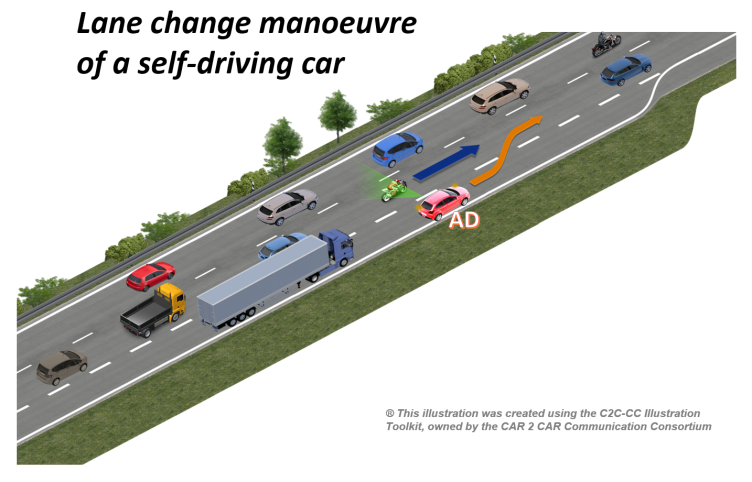
\includegraphics[width=\columnwidth]{Figures/literature_review/proposal/MotorcycleLaneChanges.png}
		\caption{C2C's Illustration of Car Changing Lanes: Representation shows that a AV may misjudge the speed of the other vehicle with limited visibility.~\cite{aecm__the_motorcycle_industry_in_europe_looking_nodate}}
		\label{fig:c2cMotorcycleLaneChange}
	\end{figure}

	\begin{figure}[htp]
		\centering
		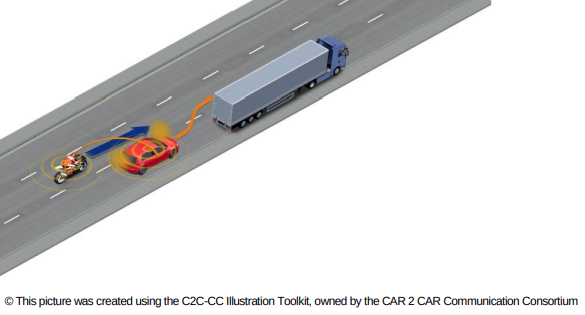
\includegraphics[width=\columnwidth]{Figures/literature_review/proposal/BlindSpotOfAnotherVehicle.png}
		\caption{C2C's Illustration of Motorcycle within Car's Blindspot: Representation displays that a AV could pull out, not detecting the motorcycle.~\cite{connected_motorcycle_consortium_application_2020}}
		\label{fig:c2cBlindspotOfAV}
	\end{figure}

\chapter{Project Objectives}
	The project involves the research, design, experimentations and findings to answer the research question. The hypothesis statements will drive the development of the study and investigations to provide a statistical analysis of any potential safety issues.

	\section{Research Hypothesis}
		This paper will cover blindspots and poor weather conditions hypothesis statements. The following hypothesis statements are orientated for the dissertation paper exploring the research question, `Are AVs a Danger to Motorcyclists?':

		\begin{enumerate}
			\item Motorcycles have blindspots that are often overlooked by human drivers, which AVs can detect and avoid.
			\item In low light conditions, AVs may struggle to accurately detect and identify motorcycles, leading to potential safety issues on the road.
			\item Poor weather conditions, such as heavy rain or poor visibility, can make it difficult for AVs to detect and react to motorcycles, increasing the risk of accidents.
		\end{enumerate}

	\section{Outline}
		The study will select relevant Machine Learning/Deep Learning (ML/DL) models, hyper-parameters and techniques, with some existing research to support the experimentation results. Some initial research papers and datasets are enclosed in this paper. However, if any new research developments are established during the experimentation, then consideration of the research would be included in the research section that backs up the investigation. The study will uncover and cover some of the existing research. However, expand on any technicalities to help prove the established hypothesis statements. The research dives into the current implementations of AVs, the training methods used to test Object Classification similarly to what is currently implemented into AVs, using a CNN model to identify the objects, and develops an understanding of the decision models provided. The model used is a Deep Belief Network (DBN) model, used to understand the context and make a filtered, educated decision based on the situation unfolding.

	\section{Aim and Objectives}
        The aim of the study is to address the problems with AVs to fulfill the research gap. The problems have been addressed within conference papers and even when it comes to object classifications. Although, with the lowest of incidents, whether it is due to the safety training of motorcyclists or population that actually ride, dependent on the country, the problem is rarely addressed thoroughly. If AVs roll out into regions like Southeast Asia: Indonesia, Vietnam, Thailand and others, and European countries: Italy, Spain, Brazil and others, then the problem will appear more, not allowing organisations to brush the problem `under the rug'. The objective is to find some theoretical logic of the underlying problems and potential solutions or considerations for Advanced Driver-Assistance System (ADAS)/AVs to adapt decreasing any potential tragic accidents.

		The main objectives of this project are to develop an accurate UK Motorcycle trained model using Ultralytic's YOLOv5 (You Only Look Once) architecture and to improve the model's performance on specific tasks. The following steps will support the experimentation to answer the research questions:

        \begin{enumerate}
            \item \textbf{Dataset Preparation:} Object Classification requires a set of labels to correspond to an image, mapping different classified objects within the image. Preparation of the data requires being able to select validated data for training and testing purposes.
            \item \textbf{Pre-processing:} Read in the mapping datasets and extract the sorted datasets to the designated file paths. 
            \item \textbf{Architecture Selection and Optimisation:} Investigate different object classification architectures, and select a model that could closely demonstrate an idea of how AVs currently initialise object classification.
            \item \textbf{Evaluation Techniques:} Confusion Matrix and PR-Curve are tools to fine-tune and evaluate the model's training performance.
        \end{enumerate}

	\section{Project Structure}
        The research during the project must justify tools to support image preprocessing, analysing and classification to provide an understanding of the problems taking place. Image preprocessing is a significant consideration in the project to answer all the hypotheses, as motorcycles may be in a blind spot, but with better adjustments, the image classification could see blur or shadows easier with sharper settings or if the time and weather have poor visibility, then dangerous the image to greyscale, and increasing edge sharpness could help make the motorcycle outline more clear. Different classification methods can improve the accuracy of a data model, including using various layers, hyper-parameters, and techniques during the training of a dataset.

        The experiment would look into image classification with the selected dataset providing information on possible misclassifications from the chosen dataset. The image classification structure would follow some standards that AVs use. However, AVs would use object classification libraries that support real-time footage. Image classification aims to see how motorcycles are identified among other vehicles to extend the research.

        Some of the strategies to determine the hypothesis statements is to select a model like DBN and CNN or R-CNN and to compare the results with the corresponding research results. Find image classification research papers for example, `An Analysis of Convolutional Neural Networks For Image Classification' researched by Neha Sharma~\cite{sharma_analysis_2018} demonstrates a good example of a CNN structure. 

        This AI project will involve seven phases in accordance with the paper `Developing ML/DL Models: A Design Framework' authored by Meenu Mary John~\cite{john_developing_2020} involving Business Case Specification, Data Exploration, Feature Engineering, Experimentation, Development, Deployment and Operational. The Business Case Specification, in this case, is to find out if motorcycles are in danger around AVs and find suggestions or research pathways to answer the hypothesis that supports the research question thoroughly. It is essential to find datasets that support the business case specifications. During the data exploration phase, exploring some available datasets and filtering them out to better back the research question is essential. 
        
        Feature engineering takes place to determine the relevant data fields or features that benefit the study. For example, non-vehicle objects like traffic lights and pedestrians are not required if the focus is on motorcycles. Although, it can be equally argued that when AVs function, they process many objects simultaneously for better awareness. 
      
        The experimentation phase includes developing a model for the dataset, compiling the model and reviewing the data to optimise the model for the dataset. This experimentation will already shape potential issues with the dataset. Each time the data is run with different tunings, it will help develop an idea of the potential issues with the dataset. 
      
        The development phase is where findings from the experimentation are presented. This phase will formalise the results and suggest to the target audience the project's future work. 
      
        The Deployment and Operational phases are not required. However, a replacement of a Review phase may be where results and findings can be discussed, and any suggestions to optimise the experimentations for future work.

	\section{Sourcing and Preparation}
		The datasets being used are arranged in YOLOv7 format and would require additional modifications to work before the training phase. The datasets that have been decided to train the models are `Motorcycle Samples - v1 VMT-V1', sourced from Roboflow~\cite{roboflow_motorcycle_nodate}, and `Road Vehicle Images Dataset', sourced from Kaggle, authored by Ashfak Yeafi~\cite{ashfak_yeafi_road_nodate}.

		The training materials are split into `images' and `labels' categories, which require some preparation. Using Python scripts, the selected training material is taken and processed together, allowing the model to see different motorcycles in different scenarios. A US and Indian dataset was used to get other road conditions and various types of motorcycles. Using the two datasets should help increase the accuracy during the training and validation process. The materials are separated and combined into a CSV file format, and another Python Snippet can reconstruct the CSV and Image Data into a new directory.

	\section{Pre-Processing}
		Three datasets would be trained using Ultralytic's YoloV5 model. The training of two daylight datasets, `Dataset A', with the filter of `bus', `car', `minivan', `motorcycle', `pickup', `scooter', `trike', `truck', `van', `person', whereas `Dataset B' involves; `motorcycle', `trike' and `person' filters. However, the third dataset, `Dataset C', uses the `Dataset A' filter with some data augmentations. Although `Road Vehicle Images Datasets' provided some night-time images that included motorcycles, the settings provided were in lit-up areas, and there were not enough night-time images,  skewing the testing results. The training images used a darkness factor of 0.5. Refer to chapter~\ref{chap:scriptingProcess}, page~\pageref{chap:scriptingProcess} for the logic reference. Unfortunately, a dataset that contained low visibility images would have been ideal, as data augmentation could include making the training images more visible and, thus, be given better feedback for data augmentation for the testing images.
			
		The `yolov5s.pts' and `yolov5l.pts' weights were applied within the training phase for both `Dataset A' and `Dataset B', with better results on the `yolov5l.pts' by 25\% when identifying motorcycles. Whereas `Dataset C' was trained on `yolov5m.pts', achieving the lowest detection rate of 67\% when detecting motorcycles in night-time instances. All training phases of the listed models used a batch of thirty-two and ten epochs.
		
		Testing materials must include video content, split into multiple frames to test the trained YOLO model, with enough images to create a strong argument. Joining a motorcycle group and exploring various routes across the United Kingdom, including motorways, dual carriageways, A-roads, and backroads, with motorcycles overtaking, filtering, and navigating blindspots, can lead to unexplored scenarios and questions that may have been previously overlooked.
					
		A decided factor is to use a Drift Innovation Ghost XL motorcycle camera attached to a motorcycle that rides within the group, then swap the camera with another rider after some time. This way, combining the content helps identify how Object Classification copes with numerous blindspots and draws some questions to further the research concerning the current safety of AV vehicles. 
		
		One sports bike and two cruisers are selected for material to test how Object Classification models handle different motorcycle styles. Ideal footage would include Scramblers, Trikes and other similar vehicles to establish how Object Classification models work in an estimated manner. A perfect material would be that during the ride out, conducted on 18$^\text{th}$ July 2023, Tuesday, would capture these vehicles, which either pass by or join us in sections of the rides. The group is instructed to overtake and be undertaken by the camera vehicle to create plenty of footage to put the YOLO model to the test.

	\section{Model Architecture}
		With the challenge of setting up a high-end model equivalent to a leading AV manufacturer like Tesla, it is essential to use detailed Object Classification training material. Using the Qualitative Research method with video frames and labels to classify the different objects in the video is required. Roboflow and other materials are outsourced and looked into using different sources in various research journals. 
			
		Using Qualitative Research methods enhances the development of engaging with better architectural concepts. Recurrent-CNN, YOLOv4 and Ultralytics YOLOv5 are looked into to achieve the model architecture for the training, validation and testing processes. After gaining access to the datasets mentioned previously, the Ultralytics YOLOv5 felt convenient to use due to the ease of data preparation and software and hardware requirements.

	\section{Evaluation Metrics}
        During the experimentation, it is necessary to discuss of how the analyst of experimental data may take place. This information will guide the project with relevant data backing up the optimisation and accuracy during the ML prototyping, and gathering feedback for the research question to present the findings and develop any potential solutions or future work.

        Two common methods of observing performance and accuracy among the different classes available within a dataset is Confusion Matrices and Classification Reports. These tools provide a clear indication of overfiting, underfitting and accuracy. The confusion matrix does this by demonstrating true positives and false positives, which the main focus to back up the research question would be the Motocycle feature to see where any false positives are detected. The Classification Report displays a range of information involving `Precision', `Recall', `F1-Score' and `Support' of each features; detailing any potential issues of outliers. Three averages: `Accuracy', `Macro Avg' and `Weighted Avg.' are included to show the overall accuracy of the model.~\cite{liang_confusion_2022}~\cite{panigrahi_deep_2018}

        As Neural Networks train with a given epoch, meaning how many iterations the test data would go through training. A history of these iterations will be on record and displayed on a `Validation and Training Loss' graph to indicate the loss gap of the initial learning and the fitness of the trained and validation data to indicate the performance and any potential improvements,~\cite{panigrahi_deep_2018}

		The Evaluation Metrics used to train the model, include the Confusion Matrix, F1-Confidence, P and R Curves, Label Correlograms to identify any potential improvements. The Ultralytic YOLOv5 Model Architecture generates these evaluation matrics in PNG image format to allow for the evaluation of the model training optimisation. The model did not generate or offer ability to allow for a classification report, which was included in the proposal to see the prediction performance. Whereas, the R-CNN architecture would have allowed for this. The Ultralytic YOLOv5 model architecture did offer hyperparameter tuning such as learning, architecture, data augmentation, loss function components, training process and other parameters. The parameters that were used and experimented to optimise the training process include:-
		\begin{enumerate}
			\item Learning Parameters.
			\begin{itemize}
				\item \textbf{lr} - (Learning Rate): The step size used in optimization.
				\item \textbf{lrf} - (Final Learning Rate): Sometimes used for learning rate annealing schedules.
				\item \textbf{momentum} - Momentum term for the optimizer, commonly used with Stochastic Gradient Descent (SGD).
			\end{itemize}
			\item Architecture Parameters.
			\begin{itemize}
				\item \textbf{depth\_multiple} - Depth scaling factor for the architecture. Found within the weights configuration file.
				\item \textbf{width\_multiple} - Width scaling factor for the architecture. Found within the weights configuration file.
			\end{itemize}
			\item Training Process.
			\begin{itemize}
				\item \textbf{epochs} - Number of epochs to train.
				\item \textbf{batch\_size} - Size of mini-batches during training.
				\item \textbf{img\_size} - Dimensions to which images will be resized for training and inference.
			\end{itemize}
		\end{enumerate}

\chapter{Legal Concerns}
\label{chap:legalConcerns}
	Legal concerns describe the current legalisation that currently impact the project, motorcycles and motorcyclists. It is equally important to look at how motorcyclists are trained legally to understand how motorcyclists may react around self-driving vehicles.

	\section{Data Collection and Usage}
		It is also important to note that gathering and publishing such materials publicly in Britain could infringe the Data Protection Act 2018 (...meeting the standards to the EU GDPR guidelines)~\cite{govuk_data_2018} law, including but not limited to:

		\begin{itemize}
			\item Must inform the member of public how the data is being used.
			\item Must allow the member of public to access personal data.
			\item Must have incorrect data updated. - This is important for the member of public to access personal data.
			\item Must allow the member of public to erase data. Which can impede the training process in one way or another.
			\item The member of public has right to stop or restrict processing of your data. - Which impacts the training process.
			\item Data portability, to allow the data to be used for different purposes.
			\item Member of public has rights to object to how your data is processed in certain situations.
		\end{itemize}

		Furthermore, member of the public has rights when it comes to automated decision-making processes (without human involvement), which could suggest Machine Learning purposes, and profiling, to predict behaviour or interests. These all matter regarding British legislation and could impede AVs from being trained in the UK when fetching video data from pedestrians, cyclists, car drivers and other motorists. This finding could indicate the lack of public datasets available for motorcyclists or any other vehicles in the UK, complicating the training process.
	
	\section{Ministry of Transport}
		The Ministry of Transport (MOT)~\cite{govuk_mot_nodate} has different requirements for a motorcycle. Motorcycles can potentially lack headlamps and primary beams and offer a range of colours; white, yellow and mainly white light with a blue tinge. Direction indicators are not required to pass the MOT if the vehicle, particularly, `do not have front and rear position lamps'. However, there are other exemptions too. Motorcycles electronics are not always reliable; in some cases, riders accept this `risk', and even though it is stated a `Minor', `Major' to `Dangerous' categories on the MOT, motorcycles may use hand signals to communicate to other road users that the vehicle is slowing down. That said, as British road users, this is a common practice we are taught if any indication equipment goes wrong to keep vehicles the road safe. British road users deal with these things subconsciously, and AVs should be expected to understand road safety rulings, especially for more vulnerable users such as motorcyclists, cyclists, and horse riders.

	\section{Rider Practices and Road Safety}
	\label{sec:lcRiderPracticesRoadSafety}
		Three critical areas of the Compulsory Basic Training (CBT), `Element B: Practical On-Site Training'~\cite{govuk_compulsory_2016}, `Element C: Practical On-Site Riding'~\cite{govuk_compulsory_2016-1}, `Element D: Practical On-Road Training Preparation'~\cite{govuk_compulsory_2016-2}, and `Element E: Practical On-Road Riding'~\cite{govuk_compulsory_2016-3}, will help how a CBT is executed during the day for trainee motorcyclists. CBT days are quartered with the said four elements, allowing trainees to complete a full training day, and trainees are encouraged to understand basic highway codes and road principles before attending. A trainee is trained by an instructor hired by an Approved Training Body (ATB).
			
		However, before going into the specifics of how a CBT is executed, it is essential to understand how the CBT works. A CBT enables a provisional learner to ride a 125CC (Cubic Capacity), restricted up to 14BHP (Braking Horse-Power) motorcycle if over the age of sixteen. If a motorcyclist is sixteen years old, then the motorcyclist is entitled to ride up to a 50cc motorcycle, which is limited to 30MPH. It is worth noting that provisional drivers, riders, and farm traffic can operate their vehicles on Dual Carriageways set to the national speed limit of seventy miles per hour. All provisional riders are not prohibited from riding with a pillion (passenger). The provisional motorcyclist falls under the \textbf{AM} category within the Provisional driver's license.
		
		\textbf{Element B} focuses on the trainee's understanding, experience and motorcycle riding skills. `Element B: Practical On-Site Training'~\cite{govuk_compulsory_2016} states the trainee must understand how the vehicle works, involving the maintenance and systems the motorcycle entails (`...does it have ABS?', `..show me the brakes, clutch and throttle'). The maintenance checks ensure the vehicle is safe on the road and give the rider the confidence to avoid any potential crashes down to mechanical failure. The section then focuses on the control of the motorcycle; the rider is trained in the following:-

		\begin{itemize}
			\item to take the vehicle off and on the side-stand or centre-stand.
			\item to slowly control the vehicle forward and bring the vehicle to a controlled stop.
			\item to start and stop the vehicle safely.
		\end{itemize}

		\textbf{Element C} teaches the trainee's control of the vehicle and observational skills. `Element C: Practical On-Site Riding '~\cite {govuk_compulsory_2016-1} mentions the use of verbal instructions on the radio to communicate manoeuvrability tasks for the trainee to execute. The trainee learns how to observe and manoeuvre out of the way of any obstacles that may exist or have developed. The trainee learns how to:-
		
		\begin{itemize}
			\item move away.
			\item ride slowly.
			\item riding in a straight line and coming to a controlled stop.
			\item riding a figure of eight.
			\item carrying out a U-turn.
			\item bringing their vehicle to a stop in an emergency.
			\item carrying out stimulated left and right-hand turns.
		\end{itemize}

		\textbf{Element D and E} takes the trainee through the basic road theory to make sure the trainee can read signs and specific hazards that may take place. The instructor then takes the motorcyclists out on the road and spends two to three hours going over the following road types, and situational areas:-

		\begin{itemize}
			\item Traffic lights.
			\item Roundabouts.
			\item Junctions.
			\item Pedestrian crossings.
			\item Gradients.
			\item Bends.
		\item Perform a U-Turn Manoeuvre.
		\item Perform an Emergency Brake Manoeuvre.
		\end{itemize}

	The following points are instilled within the rider, including how that knowledge and understanding applies in a range of real-world applications and the limits of their competence. This practical training helps motorcyclists avoid danger if they are not over-competent. This methodology helps the reader understand the mindset given to motorcyclists on British roads. It shows how a motorcyclist is trained to avoid driver error as much as possible.

\chapter{Literature Review}
\label{chap:literatureReview}
	\section{Motorcycle Legalities and Safety Regulations}
	\label{sec:lrMotorcycleLegalitiesSafetyRegulations}
		\subsection*{Motorcycle Licensing}
			The CBT takes a day or two before handing a certificate, depending on the rider's confidence on and off-road. CBTs last for two years. A CBT can cost roughly £120 and be refunded by certain councils around the UK. A provisional motorcyclist must have a valid CBT certificate to progress to a full license. The motorcyclist has to pass the Theory, practical off-road and on-road training, and practical off-road and on-road tests. The process could take a month or two to complete, and each training/test takes one day. However, the tests involve using a more considerable capacity bike and spending a whole day on off-road and on-road training and tests, compared to one day fitting the four elements into it. 

			There are three full license categories for the motorcyclist, that is also restricted to the age of the motorcyclist. These categories include an \textbf{A1}, \textbf{A2}, and \textbf{A}. The A1 license category entitles the motorcyclist, aged 17, to an unrestricted 125cc motorcycle, allowing access to the motorway and the rider to carry pillions. The A2 license category entitles the motorcyclist, aged 19, to a restricted 47BHP \textit{(or if 95BHP, can be restricted to 47BHP with certification)} motorcycle. A category license has two access entry types; the first access entry is that the motorcyclist must be twenty-four years old, or the second access entry is that after the motorcyclist holds the A2 license category for two years, then the motorcyclist can retake the practical tests, without the need for a Theory to upgrade their license. For a visual representation, refer to the UK Government's Flowchart~\cite{govuk_motorcycle_nodate}.

		\subsection*{Employing Official Instructors}
			Driving Standards Agency (DSA)~\cite{driving_standards_agency_compulsory_nodate} releases an article, `COMPULSORY BASIC TRAINING (CBT) ASSESSMENT FOR MOTORCYCLE INSTRUCTORS', to give an understanding of how ATBs select the right instructors that guarantee the safety of trainees that proceed with the CBT. DSA enforces the following statement:-
            \begin{center}
                ``DSA operates `fit and proper' criteria, which requires an individual applying to be authorised,
                to give details of any motoring or non-motoring offences not yet spent. Details of offences will
                be taken into account when assessing their suitability to be authorised as a certified
                motorcycle instructor. Applicants should, therefore, note that successful attendance on the 2-
                day CBT assessment does not provide automatic acceptance of an application to be a
                certified motorcycle instructor.'' - Driving Standards Agency~\cite{driving_standards_agency_compulsory_nodate}
            \end{center}
            
            The report states, `All Approved Training Bodies (ATB`s) must employ at least one instructor who has successfully attended the DSA assessment.', which indicates that once a motorcycle instructor passes the Motorcycle Instructor assessment, then the ATB employs a motorcycle instructor. This approach guarantees a demand and supply for the role and means motorcycle instructors are encouraged to fall into this line of work.
            
            During the assessment, the instructor is encouraged to understand `The Official DSA Guide to Learning to Ride', `The Official DSA Guide to Riding - The Essential Skills', and `The Official Theory Test for Motorcyclists', which allows the driving instructor to teach trainees with an understanding of safety when it comes to the road.

			DSA~\cite{driving_standards_agency_compulsory_nodate} provides the mindset instilled into motorcyclists, which briefly mentions the concepts involved within the CBT practices taught to the instructors. The DSA mentions the concepts explained in the section~\ref{sec:lcRiderPracticesRoadSafety}, page~\pageref{sec:lcRiderPracticesRoadSafety}, and reinforces the principles with more detailed information. This ideology can add volume to the level of detail that goes into Motorcycle Training and provides a reason that the system already available is enforced to a strong level of detail.

            To be an approved motorcycle instructor, nine steps must be completed. The first step requires to be de-briefed with the syllabus for the assessment. The second step introduces the assessment and is then told to de-brief the DSA assessor on the ongoing lesson. The third step involves the machine introduction, and in this case, the DSA assessor will simulate being a CBT Instructor, whilst the candidate will act as a learner. The candidate is then expected to de-brief the DSA assessor. The fourth to fifth step involves practical on-site training, in which the DSA assessor will act as a learner, the candidate will give the instructions to the DSA assessor, and then a de-brief will follow. The sixth to eighth step is the same principle as before, although it will be conducted on the road. The last step of the process involves receiving a full de-brief from the DSA assessor, and the assessment result is given after seven to ten days.

	\section{Autonomous Vehicle Paradigm and Legalities}
		Firstly, it is essential to understand how vision works on AV and what techniques are in place to allow vehicles to function correctly and safely. Journal Article, `AVs: from paradigms to technology', authored by Silviu Ionita~\cite{ionita_autonomous_2017}, offers underlying information about the foundation of autonomous vehicle systems. It is equally important to understand how motorcycles function within traffic and the reasoning behind motorcyclist mentality.

		Silviu Ionita~\cite{ionita_autonomous_2017} describes that for a ADAS/AV system to be `intelligent', then the system must meet the following requirements:
		\begin{enumerate}
			\item ``To learn in `teaching mode' but also from own experience. This is a necessary condition but not sufficient.''~\cite{ionita_autonomous_2017}
			\item ``To perform approximate reasoning. This suppose more than true/false logic in formal
			reasoning, it requires the use of multivalent logic that deals better with the uncertainty.''~\cite{ionita_autonomous_2017}
			\item ``To behave autonomously. This is the aggregate performance that includes many operational functions based on the first two conditions in order to put in practice the intelligence, which is equivalent with the intelligent behavior.''~\cite{ionita_autonomous_2017}
		\end{enumerate}

		Motorcycling filtering laws vary in different countries globally. Australia and USA states have different definitions of filtering. Some states declare filtering legal, whereas other states declare filtering illegal. Thailand country made filtering illegal. However, some of these states or countries where filtering is illegal are poorly policed, indicating that motorcyclists may filter if an opportunity arises. That means AV vehicles should anticipate filtering even in countries/states where filtering is illegal to minimize the number of casualties and incidents.~\cite{promraksa_lane-filtering_2022}

		An `intelligent vehicles' paradigm has three logical rule statements to follow. Firstly, the system will collect data from the driver, developing the knowledge from itself and the driver. Second, the system will have to perform some judgement. Silviu Ionita~\cite{ionita_autonomous_2017} mentions that it is paramount to filter the data through logical statements and apply multivalent logic to handle uncertainty better, creating a better judgement. ADAS require consistent autonomous behaviour to collect and handle the data even when the system is not in control. This behaviour means that the developers can collect data on what the system would have done if it were in control, allowing any refinement down the line and enabling AVs to work more efficiently.

		Figure~\ref{fig:adasFunctionsIonita} provides the structure of Advanced Driver Assistance Systems (ADAS) functions linking the responsibilities to the decision and action. Strategic Processes are near real-time, Tactical Processes are real-time, and Direct Processes are short as possible. These three functionalities are fundamental when understanding how an ADAS vehicle copes and how an AV will tend to handle situations.~\cite{ionita_autonomous_2017} It is necessary to establish that the AV will only rely on its judgement after the decision to remove human interaction. Some of these system paradigms reflect the capabilities of AVs involving blindspots, low-light and poor weather conditions.
		\begin{figure}[h]
			\centering
			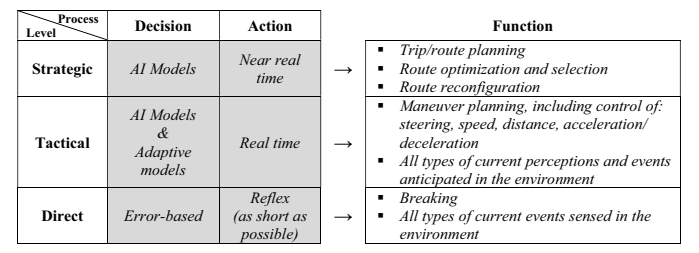
\includegraphics[width=\columnwidth]{Figures/literature_review/proposal/SystemFunctionality-3.png}
			\caption{Classes of ADAS and their Requirements for Decision and Execution~\cite{ionita_autonomous_2017}}
			\label{fig:adasFunctionsIonita}
		\end{figure}

	\subsection{Vision Technology and Techniques}
		When investigating how AVs handle blindspot handling compared to human drivers, the paper `Automated driving: Safety blind spots' by Ian Y. Noy~\cite{noy_automated_2018} suggests the current implementations within ADAS and compares it to standard driving errors. Although, the paper does not directly reflect on motorcycles, the paper details ADAS systems and how the transition from ADAS to AVs is possible. An important quote from the paper is that `AD technologies are suboptimal in that they fail to address critical blind spots and will likely lead to unnecessary losses and injuries because insufficient consideration is given to integrating the human element into overall sociotechnical road transportation system'~\cite{noy_automated_2018} suggests that transitioning from ADAS to AVs is relatively dangerous if blindspot judgements are overlooked. With further research in this area, it will provide more information to understand if AVs are safer than human drivers on the road.

		Light Detection and Ranging (LiDAR) uses a pulsed laser to gather information about the object surroundings, providing depth that images cannot capture. Within the paper, `Pedestrian recognition and tracking using 3D LiDAR for autonomous vehicle' by Heng Wang~\cite{wang_pedestrian_2017}, a quote ``LiDARs are another kind of commonly used sensors for pedestrian recognition, compared with cameras, LiDARs can provide accurate range information and larger field of view.''. Heng Wang points out that the use of LiDAR widens the field of view.
		
		After researching some extra information, it was found within the report `What Happens for a ToF LiDAR in Fog?'~\cite{li_what_2021} that the failure rate of detection in Diffuse Reflection Targets: 2.1\% and Retro-Reflective Objects: 0.7\% in the range of 0-10m, Diffuse Reflection Targets: 10.3\% and Retro-Reflective Objects: 1.1\% in the range of 10-15m, Diffuse Reflection Targets: 15.1\% and Retro-Reflective Objects: 1.1\% in the range of 15-20m, and Diffuse Reflection Targets: 19.5\% and Retro-Reflective Objects: 0.7\% in the range of 0-10m~\cite{royo_overview_2019}

		When investigating how AVs handle blindspot handling compared to human drivers, the paper `Automated driving: Safety blind spots' by Ian Y. Noy~\cite{noy_automated_2018} suggests the current implementations within ADAS and compares it to standard driving errors. Although the paper does not directly reflect on motorcycles, the paper details ADAS systems and how the transition from ADAS to AVs is possible. An important quote from the paper is that `AD technologies are suboptimal in that they fail to address critical blind spots and will likely lead to unnecessary losses and injuries because insufficient consideration is given to integrating the human element into overall sociotechnical road transportation system'~\cite{noy_automated_2018} suggests that transitioning from ADAS to AVs is relatively dangerous if blindspot judgements are overlooked. Further research in this area will provide more information to understand if AVs are safer than human drivers on the road.

	\section{Model Architectures}
		Yen-Yi Wu~\cite{wu_pedestrian_2016} suggests using a DBN model for object classification. The model correctly classifies images: pedestrians, bikes, motorcycles and other vehicles. The model thrives an 89.53\% accuracy.

		The r-CNN model merges a CNN approached model with a Region-based model to create a deeper layered one. The aim is to increase accuracy and performance regarding object classification. The R-CNN uses a selective search algorithm to find certain features within the set of images and focus on the objects that match the specified features using diverse strategies. This approach means that when training the model, it is equally important to understand what the layers do and how they filter the image to change the test data to analyse the different performances and accuracies of the training and testing.~\cite{uijlings_selective_2013}~\cite{ren_faster_2015}

		DBN model is based on Restricted Boltzmann Machine (RBM) layers to train the model. According to `An overview on Restricted Boltzmann Machines'~\cite{zhang_overview_2018} explains that RBMs pre-train the networks' weights. This technique is done layer by layer and applies gradient descent methods to fine-tune the weights. This method alone allows the neural network to optimise the hyper-parameters, which in turn boosts accuracy and optimises the model's overall performance.

		Both model suggestions both use CNN, whether it is merging CNN or comparing to CNN. The Journal Article titled "Detection of Motorcyclists without Helmet in Videos using Convolutional Neural Network" by C. Vishnu includes a layer designed to recognise whether a motorcyclist is wearing a helmet. This finding emphasises an essential feature in ensuring the safety of riders on the road. Using a Convolutional Neural Network, the layer can accurately detect whether a helmet is being worn, which can help prevent accidents and reduce injuries. It is impressive to see how technology can enhance safety measures in everyday life. The layers proposed by the author should benefit the datasets used in this research project. The layer structure is fatigue, although it involves ReLU, max-pooling, fully connected and a loss function (Support Vector Machines or Softmax) layers.
        
        Figure~\ref{fig:adasFunctionsIonita} displays the DBN and RBM layers from the paper, `Parallel computing method of deep belief networks and its application to traffic flow prediction' illustrated by Lu Zhao~\cite{zhao_parallel_2019}. DBN is not a convolutional network compared to CNN. DBN consists of a two-layer graph, including a visible layer below and a hidden layer above, displayed in figure~\ref{fig:dbnRBMLayers}. The author and illustrator mention that the RBM layers illustrated are slightly different to the classical Boltzmann Machine.~\cite{zhao_parallel_2019}

		\begin{figure}[htp]
			\centering
			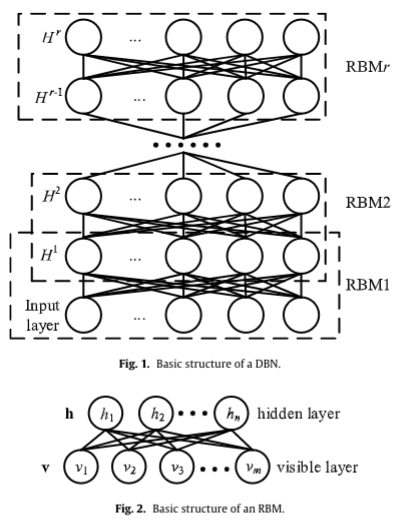
\includegraphics[width=0.75\columnwidth]{Figures/literature_review/proposal/DBNRBMLayers.png}
			\caption{DBN and RBM Model Layers~\cite{zhao_parallel_2019}}
			\label{fig:dbnRBMLayers}
		\end{figure}

	\section{Datasets and Preparation Idealogies}
		Finding the suitable dataset for the given research question involves first identifying the required information. The requirements of the dataset need to have motorcycles on the road with different situations, camera angles and visibility. After exploring through some datasets, three image classification datasets, `TuSimple'~\cite{jeong_end--end_2017}, `Car vs Bike Classification'~\cite{deepnets_car_nodate} and `MB10000'~\cite{espinosa_motorcycle_2018}. The ideal datasets at the time was `TuSimple'. However, the dataset was twenty-five gigabytes, and meant that training the dataset was too much for individual research. The `Car vs Bike Classification' dataset lacked authentic motorcycle and car images in realistic situations. However, the dataset was lightweight, with one hundred and eight megabytes. These mentioned specifications meant that the `MB10000' had an optimistic fitness to support this experiment. The dataset has realistic situations, motorcycles with other vehicles and image sequences to support image classification. The dataset has four-hundred and twenty-six megabytes of filesize.

		`Pedestrian, Bike, Motorcycle and Vehicle Classification via Deep Learning: Deep Belief Network and Small Training Set' by Yen-Yi Wu~\cite{wu_pedestrian_2016} goes over different visibility levels that affect pedestrians, bikes, motorcycles and vehicles and how image classification affects these vehicles. The image preprocessing involves converting colour images to greyscale. Including edge emphasis, detection to enhance to the image, with the fundamental aim to detect edges of objects seamlessly. The paper suggests using a fixed threshold and Otsu methods to threshold greyscale images and use bilinear interpolation for image resizing. These methods should increase the visibility of the objects within the images are good notes for when conducting any experiments.

\chapter{Research Methodology}
\label{chap:researchMethodology}
	\section{Fundamental Research}
		Fundamental research methodology builds a directive of a research area driven by curiousity. This type of research collection increases the understanding of a selected research topic, which is vital in cases where not many research papers exist. Fundamental research papers alone are not substantial to start developing towards a research project, as the name suggests, it creates a foundation and provides insights to understanding any problems found during the research study. These papers tend to cover basic understandings of phenomenon's, which in turn backs up the research question. These research materials may include surveys, interviews, observations and experiments.~\cite{saunders_research_2012}

		In the context of AVs and motorcycles, the research methodology seeks to understand any underlying principles of the interaction of these vehicle types on the road. It may even contain discussions and analytics of crash data or theoretical requirements that AV organisations should follow. For example, a study of how drivers and rider perceive each other on the road would impact the research approach, taking in account of the AVs visibility requirements. For the project, consideration of conference papers, case studies and surveys should help form any research directives to approach the testing of the hypotheses statements.

	\section{Statistical Research}
		Statistical research is a critical component of this research project, as interpreting the analytical data generated from the Neural Network is important. AVs and ADAS are complex systems, and require a good understanding of the statistics of real life events to understand hypothetical situations. The goal of statistical research is to identify patterns, relationships and trends within the data. These three variables allow the testing about each individual hypothesis and forming the conclusions of the research method.

		Statistical research could involve comparing other object classifications papers involved with AVs and motorcycles, taking account of the design plan, neural network model and layers, results and discussions to give an understanding of industry standard results. This also gives a great way to test the findings from the research project against the statistical findings and then form a detailed report of the findings, and provide a useful further work section. Statistical research has been demonstrated to make sure that the datasets are relevant and up-to-date Use Cases, and to understand the initial problems with motorcycles and ADAS/AVs to develop the research question.

	\section{Quantitative Research}
		Quantitative research involves the numerical data to collect and analyse data. This has a secondary importance similarly to the fundamental research methodology. This research collection appears a few times whether it is working with the algorithm, Confusion Matrix or understanding numerical data gathered from fundamental and statistical research papers to understand of variables in relation of AVs and motorcycles. Quantitative research methodology can help with identifying and aids with developing evidence-based recommendations for improving motorcycle safety.

		Quantitative research methodology tends to involve surveys, questionnaires and user studies. The methods enable the research to contain a large amounts of numerical data related to the research question. Numerical techniques can also provide tools to conduct correlation analysis and hypothesis testing, in accordance with research from the statistical side and experimental results. The quantitative methods has been applied to check performance, size and other key factors when it comes to preparing the Neural Network to make sure that the hypotheses are accurate and workable.

	\section{Qualitative Research}
		Qualitative research is a crucial factor of this project. As seen in this proposal, datasets had to be observed to make sure they could withstand the hypotheses. During the prototyping and evaluating of the model, observations will be made and cross-referenced to make sure that the findings are accurate. This type of testing could help work out any potential issues with current data structures or even provide some awareness of problems that may have not been considered before. It is also important to make notes from other research projects with qualitative research to consider any key points.

		In addition, observation studies could help enhance the research development. This could be finding case studies that provide videos of AVs in process with descriptions of what the program is doing and what systems are in place. This content could involve indepth interviews with experts and stakeholders to understand AVs and motorcycle's current interactions and known concerns. It could also be a useful tool communicating to some motorcycle instructors or experts to understand if there is any on-going issues with ADAS vehicles and motorcycles. These could aid the study further in seeing or hearing the experiences.

\chapter{Development Methodology}
\label{chap:developmentMethodology}
	Due to the nature of the AI project, the Agile development methodology does not fit. Although, if the project involves a team of developers, then the Agile development methodology will make the better fit. The AI project has a small team and requires a lot of repetition to find the best fit and results for the experimentation. The Iterative development methodology is the best approach. The Agile Methodology could cost anywhere from £422.91 (Freelancer Team Members) to £2085.04 (Payroll Team Members)~\cite{owais_effort_2016} 
	
	Where usually, Agile development methodology has an initial cost factor, and the development saves coordination, flexibility and performance within a team development environment. However, it does not fit in a project that aims to deliver results to address a safety issue. The Agile methodologies, Iterative and Rapid Application Development (RAD) development methodologies address this project better, with the ability to make a prototype model, test and refine it. 

	RAD is a risky methodology as it does not allow the flexibility to redesign the plans to enable definition when addressing the given safety concern. Therefore, the Iteration development model is an ideal solution, allowing the ability of initial planning and then additional planning and requirement changes, also continuously updating the analysis and design, testing and evaluation. This key methodology cycle will benefit the ideology of setting the layers up and evaluating the results. Agile Methodology also uses User Stories, which is excellent if a platform is being made. However, the user stories would get repetitive during the research project, which wastes time in this specific scenario.

	\section{Iterative Development Methodology}
		The choice of an Iterative development methodology aligns well with the project's requirements. This methodology ensures that all project materials meet the predefined milestone goals. From the traditional Iterative development methodology approach, an adaptation of Continuous Integration (CI) and a Test-Driven Development (TDD) structure allows the tests to be written before the project code to optimise workflow quality and performance. The idea of this is to accelerate the project time.

		The GitHub platform provides the project tools to carry out the Iterative development methodology, including CI tools, allowing the advantage of `code repositories', `branching strategies', `dependency management', `compilation', `linting; Python Black, and pre-commit, `automated testing', `documentation', and `project management' tools that, that really push the Iterative and CI approach forward into the workflow.

		Unit Testing and CI is a challenge for an object classification project. The purpose of Unit Testing is to create a library that is suitable for the required datasets and model architectures. The absence of Unit Testing allows for the creation of poorly modified versions of CSV datasets within the pre-processing and combination stages. The goal is to provide reliable results before beginning the actual work. Another challenge would include wasting lines of code and having to redo a backlog of issues, allowing the project to be more challenging rather than efficient. The solution involves PyTest, with a CI to ensure each push to GitHub passed the tests, and using Python Modules helped ensure reusable code. This approach meant that the code could be run in a notebook, with certainty that the code quality of the modules created was to the quality required by the set milestones and tasks at hand available from the project Kanban chart. 
		
		If a series of codes needed to change or the test did not meet the next iteration of tasks, the tests were updated before any module codes were implemented. This application of TDD proves that TDD is beneficial not only in Software or Gaming specific for productivity but also in the set rules for AI engineering and module tuning.

		The research project involved a series of automation task tracking methods available from GitHub Project, involving the use of iterations to track the iterations; milestones customised to track the elements iterations; Kanban chart allowing the movement of tasks per iteration, and a Start and End Date to allow the project's Gantt chart to work allowing the Project Stakeholders and developers to monitor to allow the timescale of the project in-check.

		The iterations on the project are set up to support the different iteration phases of the project, involving `Initial', `Data Collection and Preparation', `Iteration $n$', and `Project Close'. Each iteration is configured to support a week's timeframe per iteration and rolls over automatically as the weeks go on. Each iteration is split into four stages to support the Iterative development methodology. After some experimentation, a good way of setting up a GitHub Project to achieve this is using GitHub Project Milestones, which can be assigned to the Repository pull requests. The milestones for the project included `Project Kickoff', `Data Collection and Preparation', `Research (Iterative)', `Model Development and Training (Iterative)', `Model Evaluation and Testing (Iterative)', `Documentation and Reporting (Iterative)', and `Research Findings (Project Closed)'. The statements are listed in order of how an iteration cycle was commenced within the project, and the remarks are a combination of Scrum and Iterative development methodologies to help the tracking per Iterative development methodology whilst also keeping the workflow very compact and easy to follow for a small team environment.

		The Kanban layout allowed for the ease of an Agile approach to the project. The Kanban chart is set up in a few ways. The task columns include `Todo', `Backlog', `In Progress | WIP: 0/2', `Priority Progress | WIP: 0/2', `Testing | WIP: 0/2' and, `Done', with the use of a Work-In-Progress (WIP) limit, limiting the three columns to three number of tasks. These Agile implementations to the traditional Iterative workflow helped the project to cause any bottlenecks during the iterations.

		A reflection of the project workflow overall works for the section of trying to complete research for a small team environment and is well managed with the suggestions mentioned. However, looking into Scrum, Agile, or even DevOps and CI/CD approaches is beneficial if the team environment grows. However, if there were no additional support, such as a well-managed test environment and CI work environment, then the Iterative development methodology would be problematic in its traditional form.

\chapter{Autonomous Vehicle Legalities}
\label{chap:avLegalities}
	AVs are designed according to existing policies to ensure safety, so to gather the methodology of an AV, the Law Commision's~\cite{govuk_automated_2022} helps highlight key recommendations that help shape AV methodologies. `Automated vehicles: joint report' report from the Law Commision's~\cite{govuk_automated_2022} shows some law suggestions to benefit AV safety, including the liability of the vehicle operator.

		\section{Safety Regulations}
			`Automated vehicles: joint report' report from the Law Commision's~\cite{govuk_automated_2022} recommends two regulatory schemes to enforce AV safety, which includes verification that the AV is road worthy and a scheme that guarantees safety whilst operating that said AV.

			The report states that {pre-deployment} safety includes the approval and authorisation processes. National and international standards determine vehicle approval, including AVs, to enter the market. Before registration, an AV must undergo a series of endorsements for its systems, components, and then as a whole. A vehicle "type" can be approved for limited or unlimited production. The UK also has a scheme for individual vehicle approvals. Post-Brexit, Great Britain has more autonomy over vehicle approvals. Manufacturers aiming to integrate an Automated Driving System (ADS) can choose between international acceptance via a UNECE regulation or a new domestic AV technical approval. Regardless of the choice, the vehicle must also obtain the recent GB whole vehicle approval, which has replaced the EU's version for most motor vehicles.

			Before a vehicle is legally recognised as self-driving, it must undergo a distinct \textbf{authorisation} phase. This process is crucial to differentiate between vehicles that merely assist the driver and those that can genuinely drive themselves. After a vehicle receives approval, it may enter the market but cannot operate autonomously. It must undergo a separate authorisation stage to be regarded as self-driving, ensuring its autonomous driving systems can safely and legally control the vehicle without human intervention. The authorisation authority, initially the Vehicle Certification Agency (VCA), assesses each self-driving feature, specifies its operational domain, and determines whether it can operate with or without a user-in-charge. Once satisfied, the authority authorises the vehicle for self-driving and registers an entity as the Autonomous System Design Entity (ASDE). The process aims to distinguish between driver assistance and true self-driving capabilities for legal purposes.

			\subsection*{The Authorised Self-Driving Entity}
				An ASDE is responsible for obtaining authorisation for autonomous vehicles and can be a vehicle manufacturer, a software developer, or a partnership between the two. The ASDE must actively assess the vehicle's safety, maintain a good reputation, and possess sufficient financial resources to address regulatory actions, including recalls. To gain authorisation, the ASDE must present a safety case, which is a comprehensive argument ensuring the system's safety, and an equality impact assessment to address potential unequal impacts. The ASDE's duties include:-

                \begin{itemize}
                    \item ongoing safety assurance.
                    \item updating the vehicle to comply with road rules.
                    \item informing users about self-driving features and limitations.
                    \item ensuring data accessibility for insurers and regulators.
                \end{itemize}

                An in-use safety regulator is recommended to oversee ongoing safety and legal compliance, investigate traffic infractions, and gather data comparing automated and conventional driving. The ASDE's communication with users regarding their responsibilities and liabilities is also emphasised. The specific organisation performing regulatory functions may vary but would initially be undertaken by existing agencies like the Vehicle Certification Agency and the Driver and Vehicle Standards Agency.~\cite{govuk_automated_2022}

		\section{Liability Regulations}
			Introduction of two new roles to identify the vehicle operator, \textbf{User-In-Charge (UIC)}, and \textbf{No User-In-Charge (NUIC)}, these roles help determine whether the blame lies on the ASDE (manufacturer/developer liability) or the human operator. UICs oversee a vehicle's operation in autonomous mode, except when explicitly authorised without one. They must be physically in the vehicle, capable of taking control, and qualified and fit to drive. UICs retain responsibilities for non-dynamic driver tasks, such as ensuring passenger safety, insurance, and vehicle legality.

			\subsection*{UIC}
				While the autonomous driving system (ADS) is engaged, UICs are not responsible for dynamic driving tasks like steering or braking and are immune from dynamic driving offences unless they intentionally interfere with the ADS. However, they remain accountable for non-dynamic driver responsibilities, such as child passenger safety, accident reporting, and vehicle legality.

				Following a handover from the ADS, UICs assume the driver's role and should have a specific defence against driving offences if they couldn't reasonably prevent a violation caused by the ADS. If a UIC fails to respond to a transition demand issued by the ADS, it can be held criminally liable for subsequent vehicle actions, emphasising the importance of prompt responses to transition demands.
				
				Furthermore, there is a possibility that a driver will not react in time to transition to prevent potential accidents. Programmatically, AVs should mitigate risks to lessen the impact. However, it is not emphasised that this process is guaranteed safe and that the UIC operator should respond. However, it is not considered illegal if an operator does not transition to override the AVs, which protects the UIC operator if the software malfunctions.

				The document also addresses concerns about UICs facing medical emergencies, suggesting specific defences to driving offences in such cases. Overall, it outlines the roles and responsibilities of UICs in autonomous vehicles, highlighting legal aspects related to dynamic and non-dynamic violations, handover situations, and medical emergencies.

		\subsection*{NUIC}
			Overseeing AVs remotely presents challenges, including connectivity, cybersecurity, and equipment effectiveness. Practical communication skills are essential, especially in emergencies. The document acknowledges potential issues like information overload and operator motion sickness.

			The document outlines the licensing process for NUIC operators, requiring them to demonstrate competence, financial stability, and safety measures. Regulatory sanctions, such as civil penalties and suspension of authorisation, are in place to enforce compliance. Emphasis is placed on safety and accountability in AV operations.
			
			Addressing passenger services in AV without human drivers, the document recommends the issuance of interim passenger permits. These permits aim to gather evidence on safety and accessibility and whether fares are charged. Local authorities' involvement is crucial to align services with regulations.

	\section{Summary of the Defined Proposals}
		The proposed safety regulations are brought forward to ensure AVs are developed and operated by traffic laws, providing awareness and appropriate avoidance procedures. The reports provide key recommendations to shape the AV methodologies and settle the liability side, eliminating the grey area of defining an operation.

		\subsection*{Safety Regulations}
			The two recommendations of the regulatory schemes implement the AV safety before they are released, to the releasement of the vehicle to the members of the public. Pre-deployment security requires approval and authorisation for an AV to be released on the roads. This security phase requires the vehicle to pass appropriate tests to identify as a self-driving vehicle. ASDE aims to ensure safety assurance, updating the vehicles to comply with road rules, user communication, and data accessibility.
	
		\subsection*{Liability Regulations}
			The introduction of UIC and NUIC determines whether the vehicle operator, manufacturers, and developers are to blame for any liability. This directive helps insurance, legal teams, and courts know where their clients stand and helps settle a potentially clear-cut case that's harder to identify with the new systems. UICs are not responsible for dynamic driving tasks when ADS is engaged, and UICs can be held criminally for due care and attention.

\chapter{Autonomous Vehicle Methodology}
\label{chap:autonomousVehicleMethodology}
	\section{Testing Methodology}
		A proposed testing methodology by Mohammad Hejase~\cite{hejase_methodology_2020} uses research, testing and simulation methods to verify that the model is fit for purpose. The fundamental process involves scenario specification, functional decomposition and a system representation using a Hybrid State System (HSS) to simulate an AV behaviour. HSS applies a Discrete Event System (FBS), Low-level Control, and System Model. Each HSS process is filtered through testing layers, including Unit, Integration, and Scenario Testing. Unit Testing includes the testing of individual low-level functions. Whereas Integration Testing for units that require transactional definitions. Scenario Testing focuses on generating scenarios to cover a range of system operations. These proposed methods are an excellent general combination when officially implementing driving methods within an AV. However, this methodology is not officially implemented. It does show a level of detail of fundamental processes that ensure that situational testing is validated and accurate, which does come under the assumption that AVs follow a similar methodology pattern during development.
		\begin{figure}[ht]
			\centering
			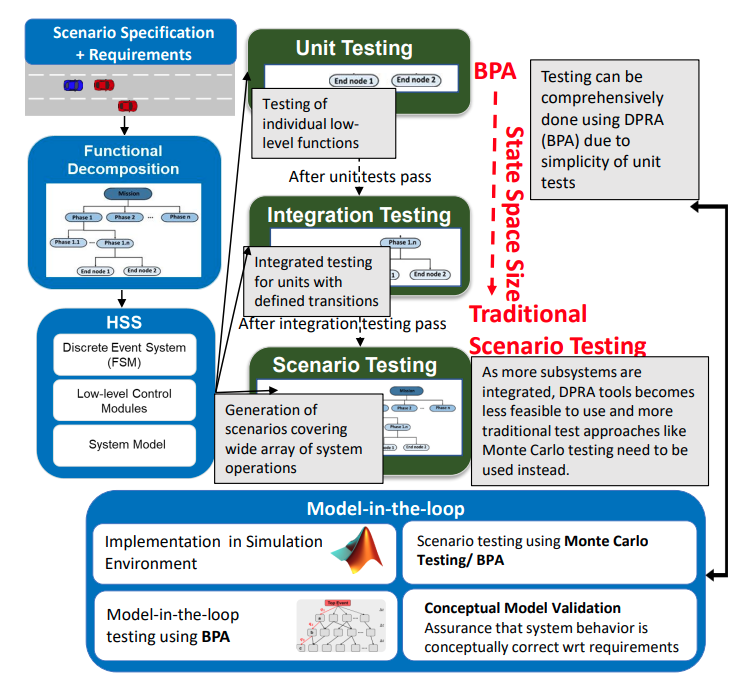
\includegraphics[width=.60\columnwidth]{Figures/literature_review/Research/Testing_Methodology.png}
			\caption{Testing Methodology: Block Diagram of the Proposed Model-Based Testing
			Methodology. Proposed and tested by Mohammad Hejase~\cite{hejase_methodology_2020}}
			\label{fig:avmTestingMethodology}
		\end{figure}

	\section{Model Methodology}
		Using Christos Katrakazas~\cite{katrakazas_new_2019} research within the Using Christos Katrakazas~\cite{katrakazas_new_2019} research within the Journal Article, `A new integrated collision risk assessment methodology for autonomous vehicles', talks about the levels of layers available within AVs model architecture. Christos Katrakazas~\cite{katrakazas_new_2019} mentions Hidden Markov Models (HMMs) and Kalman Filter Models (KFMs). These models are optimised to analyse situations and data problems in finite time windows. These models handle discrete and multivariate input and output, which can be easily extended. Christos Katrakazas~\cite{katrakazas_new_2019} mentions that HMMs have high sample and computational complexity, making learning and probability inference time-consuming. Simple HMMs also struggle with dynamic environments like traffic scenes because they rely on a single discrete random variable.

		DBNs involve a three dimensional layering system, where each row has a unique function. The layers of a typical Deep Belief Network (DBN) are as follows:
		\begin{enumerate}
			\item \textbf{Layer 1 (Contextual Level):} This layer represents the vehicle's motion context and includes a symbolic representation of the vehicle's state. It contains information about the vehicle's manoeuvre or the relationships between vehicles. The variables in this layer, such as the type of manoeuvre or adherence to traffic rules, are typically discrete and hidden.~\cite{katrakazas_new_2019}
			\item \textbf{Layer 2 (Physical State Level):} This layer relates to the vehicle's physical state, including its kinematics and dynamics. It includes information like position, speed, and heading, and might also incorporate data from a dynamic motion model, such as the bicycle model. The variables in this layer, such as speed, position, and acceleration, are typically continuous and hidden.~\cite{katrakazas_new_2019}
			\item \textbf{Layer 3 (Sensor Measurement Level):} This layer represents the raw sensor measurements. The data is processed to remove any noise and derive the physical state. The variables at this level are always observable.~\cite{katrakazas_new_2019}
		\end{enumerate}

		During the DBN process, the data is given context, moved to the physical state, and then filtered back to the context layer to provide a new context for the state. Eventually, this data that is being filtered will be pushed to the observation layer, which provides the result of what the model decided to do with the data. Furthermore, this model is responsible for taking in the scenario and giving an educated response from the available road context and physical state of the vehicle to decide the best action available.
		\begin{figure}[ht]
			\centering
			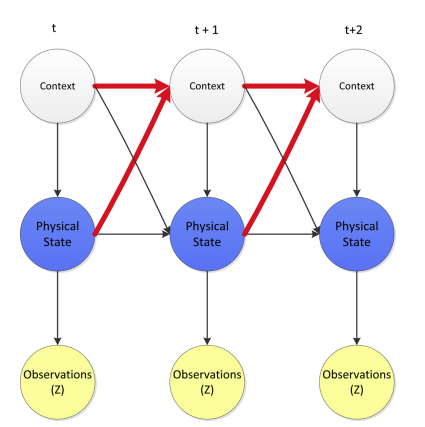
\includegraphics[width=.60\columnwidth]{Figures/literature_review/Research/DBN_Model.png}
			\caption{Model Methodology: Graphical representation of a typical DBN-based interaction aware. Illustrated by Christos Katrakazas~\cite{katrakazas_new_2019}}
			\label{fig:avmModelMethodology}
		\end{figure}

		This finding helps to understand the interaction layer of the AV when it is in self-driving mode. It gives an idea of the complexity of the current AV models, how they perceive traffic, and situational events if the vehicle is given a potential hazard event to avoid. This research helps understand the level of detail in place to prevent any life-threatening road collisions with road users.

	\section{Operational Methodology}
		Silviu Ionita~\cite{ionita_autonomous_2017} shows the basic AV methodology fabricated from the ADAS functionality to give an understanding of how a AV prioritises the driving tasks. 
		
		The diagram shown in fig~\ref{fig:avmOperationalMethodology-SF1} displays the details involved with the AV operational methodology, involving the safety methodology of basic tasks and functions of vehicle driving. The `Vehicle Driving' involves the `Rules, Knowledge and Models'; splitting down to three processes, \textbf{navigation}, \textbf{monitoring and processing of driving environment}, and \textbf{maneuver and dynamics control}. These processes are cruicial when it comes to navigating the vehicle on roads, taking in account traffic rules and regulations, whilst also monitoring potential hazards, dangers, and calculating other road users actions.

		The navigation process focuses on the planning, optimisation, route selection and reconfiguring of the vehicle's directives. At the same time, the monitoring and processing of driving environment filters focuses on the perception of road signs and markings, situational events such as legal signals, traffic lights, traffic agents and pedestrians, and perception of events such as the sudden appearance of any hazards to prevent incidents. Finally, the manoeuvre and dynamics control involves the vehicle's steering, distance, speed/acceleration and braking. 

		Figure~\ref{fig:avmOperationalMethodology-SF2} shows the structure of how ADAS currently functions, using a three-way knowledge including unsupervised and supervised features. This information includes a Deep Learning model, CNN, and human intelligence. This concept includes human intuitive reasoning and expert input. Deep Learning and expert knowledge are used to create structured knowledge and formal reasoning to provide driving actions. Intuitive reasoning is the driver stepping in to override the self-driving principles to input the driving actions to avoid potential accidents, ensuring the reduced risk of fatalities.
		\begin{figure}[ht]
			\centering
			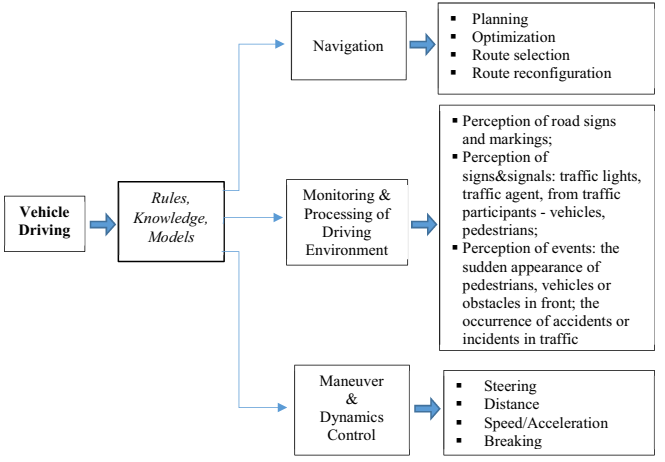
\includegraphics[width=.60\columnwidth]{Figures/literature_review/proposal/SystemFunctionality-1.png}
			\caption{Safety Methodology: Basic tasks and functions of vehicle driving~\cite{ionita_autonomous_2017}}
			\label{fig:avmOperationalMethodology-SF1}
		\end{figure}

		\begin{figure}[hb]
			\centering
			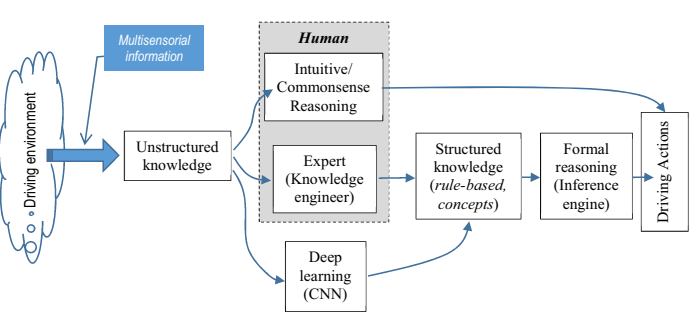
\includegraphics[width=.60\columnwidth]{Figures/literature_review/proposal/SystemFunctionality-2.png}
			\caption{Safety Methodology: Three ways of knowledge usage in driving actions~\cite{ionita_autonomous_2017}}
			\label{fig:avmOperationalMethodology-SF2}
		\end{figure}


\chapter{Scripting Process}
\label{chap:scriptingProcess}
	For the scripting process to successfully achieve the given experiments to the given workflow mentioned previously, all have a role in making this project successful. The workflow helped provide a consistent format and guaranteed successful builds and tests. The libraries helped achieve the results during each step and played a vast role in saving time in the pre-processing section of the project. The development process allowed the creation of libraries to make modules that could be executed within a notebook, allowing a step-by-step process when starting from scratch. Notebooks are designed to create the given datasets and testing tools, allowing the ML engineering phase to commence to train the given models.

	\section{Libraries}
		The libraries that formulate the workflow to allow system functionality, code quality and testing, data manipulation and analysis, machine learning and data modelling, image processing, and interactive development processes are listed below, briefly explaining why they were used.

		\subsection*{System Functionality}
			YOLOv5 datasets use a file system technique to store each video frame; these images are stored in `images/'. The labels identify the objects within txt format, stored in `labels/', with a `data.yaml' configuration file to help YOLOv5 architecture understand where the file locations are, including what and how many classes exist. The purpose of the configuration file is to map the class IDs from YOLOv5 text labels to the corresponding configuration class names. The formats gathered from Roboflow were already split into `train/', `test/', and `val/'. The `os' library helped with file reorganisation techniques.

		\subsection*{Code Quality and Testing}
			This project involves the practice of an iterative development methodology complemented by Continuous Integration (CI) practices to run this project. This strategy is to help prevent the code quality from deteriorating over time and any backlogs that may start stacking up, with the use of a TDD environment and CI modifications. `flake8' Python library prevents any bad styles found within the code, like any possible syntax errors or bad coding practices to keep the code consistent and clean. `black' Python library formats the code to a given house-style setting from a configuration file, which makes the code easier to read. The Python library, `pytest', allows configuring the testing environment. The `pre-commit' module hooked the `black' code format library if `flake8' reports any errors when `git commit' is called. Finally, a CI was set up on GitHub to install Python and run the tests to test if the project was eligible for any merges, which was updated on Kanban. This process allowed for automated tasks and ensured positive project quality.
		

		\subsection*{Data Manipulation, Machine Learning, Image Processing and Data Modelling}
			Data manipulation libraries are essential for DL practices. `numpy' and `pandas' are powerful libraries. `pandas' offer data structure tools to help load CSV data into memory. Where `numpy' offers numerical computations in Python. These are used in multiple areas, including the loading and combination of different datasets together. The use of `cv2' and `numpy' allowed converting a daylight image dataset into a night-time image dataset, which helped the training phase of `Dataset C'.

			`Tensorflow' and `Keras', including splitting the image data to `train/', `test/' and `val/' categories, and pre-processing images. These helped choose a random series of images and labels from the combined dataset and train the model, giving a decent amount of test images to see the training outcome. `Pillow' was a library used to create fake images for the testing phases, and reading images into the notebook
		
	\section{Testing and Implementation}
		Developing the code in this project involved reading through the following current tasks and creating a test that would fail, with a brief description. The aim was to get the test to pass at a bare minimum, then review the following stages. This methodology meant the test was built over time and worked well during development. This method guaranteed that any outcome of the test would be as expected and changed the dynamics of the development process. Python modules in `./workbench/modules' were used in the tests. If a function existed in a notebook or for testing purposes, a test was not wasted on the tasks. The form of testing used was component tests. However, there are aspects of unit testing in cases where component testing was insignificant.

		\begin{lstlisting}[tabsize=1]
			import unittest
			import os
			import csv
			from PIL import Image
			import tempfile
			from modules.pre_processing.CSV_Creation_YOLO import (
				read_image,
				read_labels,
				normalise_labels,
				get_config,
				get_data,
			)

			from modules.pre_processing.CSV_PreProcessor import preprocess_to_csv


			# YOLO uses <object-class> <x> <y> <width> <height> classification labels to identify the frames.
			# The test case ensures that the methods implemented will work properly for YOLO classification.
			class TestPreprocessing(unittest.TestCase):
				def setUp(self) -> None:
					# Create a temporary directory
					self.test_dir: str = tempfile.mkdtemp()

					# Create images and labels subdirectories
					self.images_dir: str = os.path.join(self.test_dir, "images")
					self.labels_dir: str = os.path.join(self.test_dir, "labels")
					os.makedirs(self.images_dir, exist_ok=True)
					os.makedirs(self.labels_dir, exist_ok=True)

					# Create a dummy config file
					self.config_path: str = os.path.join(self.test_dir, "data.yml")
					with open(self.config_path, "w") as f:
						f.write("names: ['car', 'bus', 'motorcycle']\nnc: 3")

					# Create a dummy image file in the images subdirectory
					self.image_path: str = os.path.join(self.images_dir, "image.jpg")
					image: Image = Image.new("RGB", (100, 100))
					image.save(self.image_path)

					# Create a dummy label file in the labels subdirectory
					self.label_path: str = os.path.join(self.labels_dir, "image.txt")
					with open(self.label_path, "w") as f:
						f.write("0 0.5 0.5 0.2 0.2\n2 0.7 0.7 0.3 0.3")

					# Define output_path as a temporary CSV file
					self.output_dir: str = os.path.join(self.test_dir, "output.csv")

				# Test 1: Failed (No Implementation)
				# Test 2: Passed (Implemented)
				def test_read_labels(self) -> None:
					labels: list = read_labels(self.label_path)
					self.assertEqual(len(labels), 2)
					self.assertEqual(labels[0], (0, 0.5, 0.5, 0.2, 0.2))

			if __name__ == "__main__":
				unittest.main()
		\end{lstlisting}

		The nature of component testing means that after a component is passed, the component has confidence that it will work successfully within a production environment. This process quickened up the development process and meant that once any merge requests were finalised, the development process for the Notebooks could commence. 

		The modules to achieve the experiment objectives include:-
		\begin{itemize}
            \item \textbf{CSV\_PreProcessor} - Providing the modules to \textbf{load}, \textbf{preprocess}, \textbf{combine} to a CSV. Other tools included loading and pre-processing an image, which allowed for the CSV Creation phase. This module design allows leeway to put the necessary `Image Path' and `Label' in a CSV file to be converted into YOLO or another format later. \textbf{Note:} At this stage, Ultralytics YOLOv5 and R-CNN architectures were on the table.
            \item \textbf{CSV\_Creation\_YOLO} - Providing the models to read existing YOLO data and create new YOLO datasets.
            \item \textbf{CSV\_Conversion} - Uses the \textbf{CSV\_Creation\_YOLO} module to convert the combined unformatted CSV data and then compile it into YOLO or RCNN format, depending on the arguments provided.
            \item \textbf{CSV\_Night} - Offers the conversion from day to night based on the paths provided. The formula is `np.clip(image * darkness factor, 0, 255)' to get a false night feel.
			\item \textbf{CSV\_TrainTestSplit} - Holds two features: TrainTestSplit function that works with YOLO to move the relevant files over, and a function to provide a feature to move files, with the use of a list of files, output directory and target subdirectory.
        \end{itemize}

	\section{Notebooks | Training}
		Five notebook components were required to gather the data necessary for the training process. These includes `DS\_ReGroup', `CSV\_Creation', `CSV\_NightMode', and `CSV\_TrainTestSplit' notebooks.

		\subsection*{Dataset Re-Group Notebook}
			The code of the notebook:
			\begin{lstlisting}[tabsize=1]
				# Note: Scripts doesn't fully support 'Traffic.zip', copy the contents within traffic_data into ../ (root directory)

				# Script contains a clean_up module, so that empty sub_directories are removed.

				# Note: Rename 'Motorcycle Samples...' to 'Roboflow', and 'traffic' to 'Traffic', otherwise other scripts will fail!

				# If interested in applying different datasets and models, create an issue to show interest, and a config file will be added to roadmap, to make the project universal. #

				# Block 1
				import os
				import shutil


				def group_files(base_dir, exts, new_folder):
					new_dir = os.path.join(base_dir, new_folder)
					if not os.path.exists(new_dir):
						os.makedirs(new_dir)

					for root, dirs, files in os.walk(base_dir):
						for file in files:
							if file.split(".")[-1] in exts:
								old_file_path = os.path.join(root, file)
								new_file_path = os.path.join(new_dir, file)
								shutil.move(old_file_path, new_file_path)


				def clean_up(base_dir):
					for root, dirs, files in os.walk(base_dir):
						for file in files:
							if file == "labels.cache":
								file_path = os.path.join(root, file)
								os.remove(file_path)

					for dirpath, dirnames, filenames in os.walk(base_dir, topdown=False):
						for dirname in dirnames:
							dir_path = os.path.join(dirpath, dirname)
							if not os.listdir(dir_path):
								os.rmdir(dir_path)

				# Block 2
				base_dir = "../../datasets/raw/Roboflow"
				group_files(base_dir, ["png", "jpg", "jpeg", "gif"], "images")
				group_files(base_dir, ["txt"], "labels")
				clean_up(base_dir)

				# Block 3
				base_dir = "../../datasets/raw/Traffic"
				group_files(base_dir, ["png", "jpg", "jpeg", "gif"], "images")
				group_files(base_dir, ["txt"], "labels")
				clean_up(base_dir)
			\end{lstlisting}

			This notebook aims to find the YOLOv5 datasets under `/raw/Roboflow' and `/raw/Traffic'. Once the datasets are found, the notebook finds all images that use one of the following formats: PNG, JPG, JPEG, GIF, and moves the images to the `images/' directory. The same thing is applied to labels. However, the program finds the `TXT' format and moves the files into `labels'. This notebook sorts the YOLO datasets, groups all images and labels, and calls the clean\_up function to delete the `train/', `test/' and `val/' empty directories. This method allows the combination of the two datasets to commence.

		\subsection*{CSV Creation}
			The code of the notebook:
			\begin{lstlisting}[tabsize=1]
				# Block 1
				allowed_classes = [
					"bus",
					"car",
					"minivan",
					"motorcycle",
					"pickup",
					"scooter",
					"trike",
					"truck",
					"van",
					"person",
				]

				# allowed_classes = ["motorcycle", "trike", "person"] # comment out if you want to train for all above

				# Block 2
				from path import *
				from modules.pre_processing.CSV_PreProcessor import preprocess_to_csv

				input_dir = "../../datasets/raw/Roboflow/"
				output_file = "../../datasets/csv/mapping/roboflow.csv"

				preprocess_to_csv(input_dir, output_file, allowed_classes)

				# Block 3
				import path
				from modules.pre_processing.CSV_PreProcessor import preprocess_to_csv

				input_dir = "../../datasets/raw/Traffic/"
				output_file = "../../datasets/csv/mapping/traffic.csv"

				preprocess_to_csv(input_dir, output_file, allowed_classes)

				# Block 4
				import path
				from modules.pre_processing.CSV_PreProcessor import combine_csv

				input_dir = [
					"../../datasets/csv/mapping/roboflow.csv",
					"../../datasets/csv/mapping/traffic.csv",
				]
				combine_csv(input_dir, "../../datasets/csv/mapping/prepared.csv")
				
				# Block 4
				# Creates the YOLOv5 Configuration
				import pandas as pd

				df = pd.read_csv("../../datasets/csv/mapping/prepared.csv")

				df["class_name"] = df["Label"].apply(lambda x: x.split()[0])

				class_names = df["class_name"].unique()

				names_string = ", ".join(f"'{name}'" for name in class_names)
				data_string = f"nc: {len(class_names)}\nnames: [{names_string}]"

				with open("../../datasets/csv/mapping/prepared.yaml", "w") as f:
					f.write(data_string)
			\end{lstlisting}

			This notebook does a few unique things regarding the preparation phase. Firstly, notice the filter options; this is how the filter between motorcycle, trike and person is selected as optional. The active filter eliminates some original vehicle objects, such as `rickshaw', as these vehicles are not found on British roads. Secondly, the notebook converts the `Roboflow' and `Traffic' datasets and filters out any given vehicle objects that are not required for the experiment. The pre-processed data is stored in both `roboflow.csv' and `traffic.csv', simply mapping the image path and the label next to the image path, allowing the TXT files not required. The label structure uses `<labelname center\_x center\_y width height>' to identify the bounding box surrounding the object.

			\begin{lstlisting}[tabsize=1]
				Image Path,Label
				../../datasets/raw/Roboflow/images/2022_0310_161409_048A-c1002_jpg.rf.1c9a31387bf99de4d1af59361d220eac.jpg,motorcycle 0.363281 0.1875 0.0484375 0.0328125
				../../datasets/raw/Roboflow/images/2022_0310_161409_048A-c1002_jpg.rf.1c9a31387bf99de4d1af59361d220eac.jpg,person 0.361719 0.15 0.021875 0.0320312
			\end{lstlisting}

			CSV Creation notebook calls the last code snippet to combine the two mappings CSV files finally. It is done by combining `roboflow.csv' and `traffic.csv' together and then creating a YOLOv5 configuration file, `prepared.yaml', which helps keep a record of the recorded classes and number of classes rather than anything in particular. The code block below demonstrates the `prepared.yaml' contents:
			\begin{lstlisting}[tabsize=1]
				nc: 10
				names: ['motorcycle', 'person', 'trike', 'van', 'pickup', 'bus', 'car', 'truck', 'minivan', 'scooter']
			\end{lstlisting}

		\subsection*{CSV Conversion}
			The code of the notebook:
			\begin{lstlisting}[tabsize=1]
				# Block 1
				from path import *
				from modules.pre_processing.CSV_Conversion import csv_to_model_format

				input_dir = "../../datasets/csv/mapping/prepared.csv"
				output_dir = "../../datasets/model/output.yolo/labels"

				csv_to_model_format(input_dir, output_dir)

				# Block 2
				import pandas as pd

				df = pd.read_csv("../../datasets/csv/mapping/prepared.csv")


				sub_dirs = ["train/", "valid/", "test/"]

				df["class_name"] = df["Label"].apply(lambda x: x.split()[0])

				class_names = df["class_name"].unique()

				data_string = f"train: {sub_dirs[0]}\nval: {sub_dirs[1]}\ntest: {sub_dirs[2]}\n\n"

				names_string = ", ".join(f"'{name}'" for name in class_names)
				data_string += f"nc: {len(class_names)}\nnames: [{names_string}]"

				with open("../../datasets/model/output.yolo/data.yaml", "w") as f:
					f.write(data_string)

				# Block 3
				import shutil
				import os
				import pandas as pd


				df = pd.read_csv("../../datasets/csv/mapping/prepared.csv")

				image_paths = df["Image Path"].values

				dest_dir = "../../datasets/model/output.yolo/images/"

				os.makedirs(dest_dir, exist_ok=True)

				for image_path in image_paths:
					source_path = os.path.join("../../datasets/raw/", image_path)

					if os.path.exists(source_path):
						shutil.copy2(source_path, dest_dir)
			\end{lstlisting}

			The first snippet focuses on processing the `prepared.csv' file, and converts the combined CSV to the YOLOv5 format. This moves the relevant text labels found in the `prepared.csv' and appends them to a text file, that corresponds to the frame name, storing them into `output.yolo/labels/' directory. The contents of the output file of\\`02\_jpg.rf.65a084066fc353cd023eb5c953f40efe.txt':

			\begin{lstlisting}[tabsize=1]
				2 0.954688 0.689252 0.0859375 0.116822
				3 0.721875 0.560748 0.0953125 0.114486
				2 0.367188 0.663551 0.05625 0.10514
				0 0.282813 0.481308 0.0171875 0.0373832
				0 0.401562 0.53271 0.01875 0.0490654
				0 0.675 0.476636 0.0234375 0.0397196
				0 0.696875 0.46028 0.0171875 0.0303738
				0 0.339062 0.331776 0.0078125 0.0140187
				0 0.401562 0.308411 0.00625 0.00934579
				0 0.478125 0.331776 0.0078125 0.0163551
				4 0.315625 0.308411 0.0140625 0.0233645
				5 0.282813 0.299065 0.01875 0.0373832
				5 0.279687 0.273364 0.0171875 0.0140187
				2 0.329688 0.436916 0.021875 0.046729
				2 0.30625 0.380841 0.0171875 0.0303738
				2 0.495312 0.39486 0.021875 0.0350467
				2 0.43125 0.343458 0.0125 0.0257009
				6 0.367188 0.415888 0.03125 0.0327103
				6 0.304688 0.336449 0.0171875 0.0233645
				6 0.415625 0.315421 0.0171875 0.0186916
				6 0.371875 0.315421 0.0140625 0.021028
				6 0.323437 0.292056 0.0078125 0.00934579
				6 0.3125 0.273364 0.0078125 0.00934579
				6 0.339062 0.280374 0.009375 0.0116822
				6 0.303125 0.294393 0.00625 0.0116822
				2 0.390625 0.310748 0.009375 0.0163551
				6 0.357812 0.348131 0.0203125 0.0257009
				2 0.360938 0.287383 0.0046875 0.0116822
				5 0.5125 0.359813 0.0515625 0.0443925
			\end{lstlisting}
			
			
			The second snippet focuses on the creation of the `data.yaml' configuration file for YOLOv5. The output file looks like this:

			\begin{lstlisting}[tabsize=1]
				train: train/
				val: valid/
				test: test/

				nc: 10
				names: ['motorcycle', 'person', 'trike', 'van', 'pickup', 'bus', 'car', 'truck', 'minivan', 'scooter']
			\end{lstlisting}
		
			Before continuation, the first top objects are trike, van, and trike objects, as the ID from the label corresponds with the object name found in the configuration file. The third snippet copies the images found in the mapping file, and copies the relevant images over to `output.yolo/images', which completes the YOLOv5 file.

		\subsection*{Night-Time Modification}
			The code of the notebook:
			\begin{lstlisting}[tabsize=1]
				from path import *
				import os
				from modules.pre_processing.CSV_Night import apply_image_modifications

				output_dir = "../../datasets/model/output.yolo/"
				sub_dirs = ["train", "valid", "test"]

				image_paths = []

				for sub_dir in sub_dirs:
					images_sub_dir = os.path.join(output_dir, sub_dir, "images")
					if os.path.exists(images_sub_dir):
						image_files = [f for f in os.listdir(images_sub_dir) if f.lower().endswith('.jpg')]
						image_paths.extend([os.path.join(images_sub_dir, image_file) for image_file in image_files])

				apply_image_modifications(image_paths, darkness_factor=0.5)
			\end{lstlisting}

			This snippet scans the image files available inside the YOLOv5 dataset prepared in the last step. The image paths are stored in memory and passed over to the image modification modules prepared previously, and darkened the image files by point five darkness factor.

		\subsection*{Train Test Split | YOLOv5 Style}
			The code of the notebook:
			\begin{lstlisting}[tabsize=1]
				# Block 1
				# open the config file
				from path import *
				import os
				import yaml
				from modules.pre_processing.CSV_TrainTestSplit import yolo_train_test_split, move_files

				output_dir = "../../datasets/model/output.yolo/images"

				# Safe Load seems to be a decent method for those that do not trust the repository in sense of loading the data #
				with open(os.path.join(output_dir, "../", "data.yaml"), "r") as file:
					yaml_data = yaml.safe_load(file)

				sub_dirs = [yaml_data["train"], yaml_data["val"], yaml_data["test"]]

				# Block 2
				train_files, val_files, test_files = yolo_train_test_split(output_dir)

				# Block 3
				import os

				sub_dirs = ["train/", "valid/", "test/"]
				output_dir = "../../datasets/model/output.yolo/"
				move_files(train_files, output_dir, sub_dirs[0])
				move_files(val_files, output_dir, sub_dirs[1])
				move_files(test_files, output_dir, sub_dirs[2])

				os.rmdir(os.path.join(output_dir, "images/"))
				os.rmdir(os.path.join(output_dir, "labels/"))
			\end{lstlisting}

			The three blocks of codes perform a simple test, train and split operation by SciKit-Learn. This process is important to train a architectural model, it selects a random selection of images, labels, splitting them into train, test and validation materials. The start of the application loads up the `data.yaml' file to find out the train, test and validation directories. The last block moves the files in the chosen directories assigned to them. This is the last process, and the YOLOv5 is now ready to be trained. 

	\section{Notebooks | Testing}
		\subsection*{Video to Frames}
			The code of the notebook:
			\begin{lstlisting}[tabsize=1]
				from path import *
				from modules.video_processing.video_to_image import video_to_frames

				# Change Paths to Absolute Location
				video_path = "/home/skira21/University of Wales Trinity St. Davids/MSc/Year 4/Project/test_videos/MISC_MP4/NIGHT2.mp4"  # replace with your video path
				output_dir = "/home/skira21/University of Wales Trinity St. Davids/MSc/Year 4/Project/test_videos/NIGHT_T2"  # replace with your output directory

				video_to_frames(
					video_path, output_dir, sample_name="Night_t2", limiter=720, start_time=0, end_time=120
				)
			\end{lstlisting}

			The path variables use absolute rather than relative paths, allowing open-source researchers to modify and convert test videos into frames easily. This project uses a third-party tool, Ultralytics YOLOv5, to train and test the files. It is imperative to code each library to adjust output paths so that users can efficiently train and test the model.

\chapter{Training Process}
\label{chap:trainingProcess}
	\section{Confusion Matrices}
		Figures (\ref{fig:ukDatasetYolov5LargeWeight},~\ref{fig:mtpDatasetYolov5LargeWeight},~\ref{fig:ntDatasetYolov5MediumWeight}) display a confusion matrix for `Dataset A', `Dataset B', and `Dataset C'. The confusion matrix shows a clear sign of any outliers. According to the Confusion Matrices, the motorcycle had an 81\% accuracy within fig~\ref{fig:ukDatasetYolov5LargeWeight}, with 39\% outliers identifying motorcycle objects as Scooters, with a minimum of 15\% outliers identifying as background. Compared to the Motorcycle, Trike and Person model, found in fig~\ref{fig:mtpDatasetYolov5LargeWeight}, the motorcycle had a 77\% accuracy, with 32\% of outliers identifying as background. Dataset C, found in fig~\ref{fig:ntDatasetYolov5MediumWeight} showed the lowest accuracy, with the datasets having a much darker vision, having a 67\% accuracy, with outliers falling into `trike' and `background' categories, with 2\% falling into `trike', and 24\% falling into `background' classifications. Although, it is impressive that the dataset had less of a chance than Dataset B to misidentify motorcycles for background noise.

		\begin{figure}[ht]
			\centering
			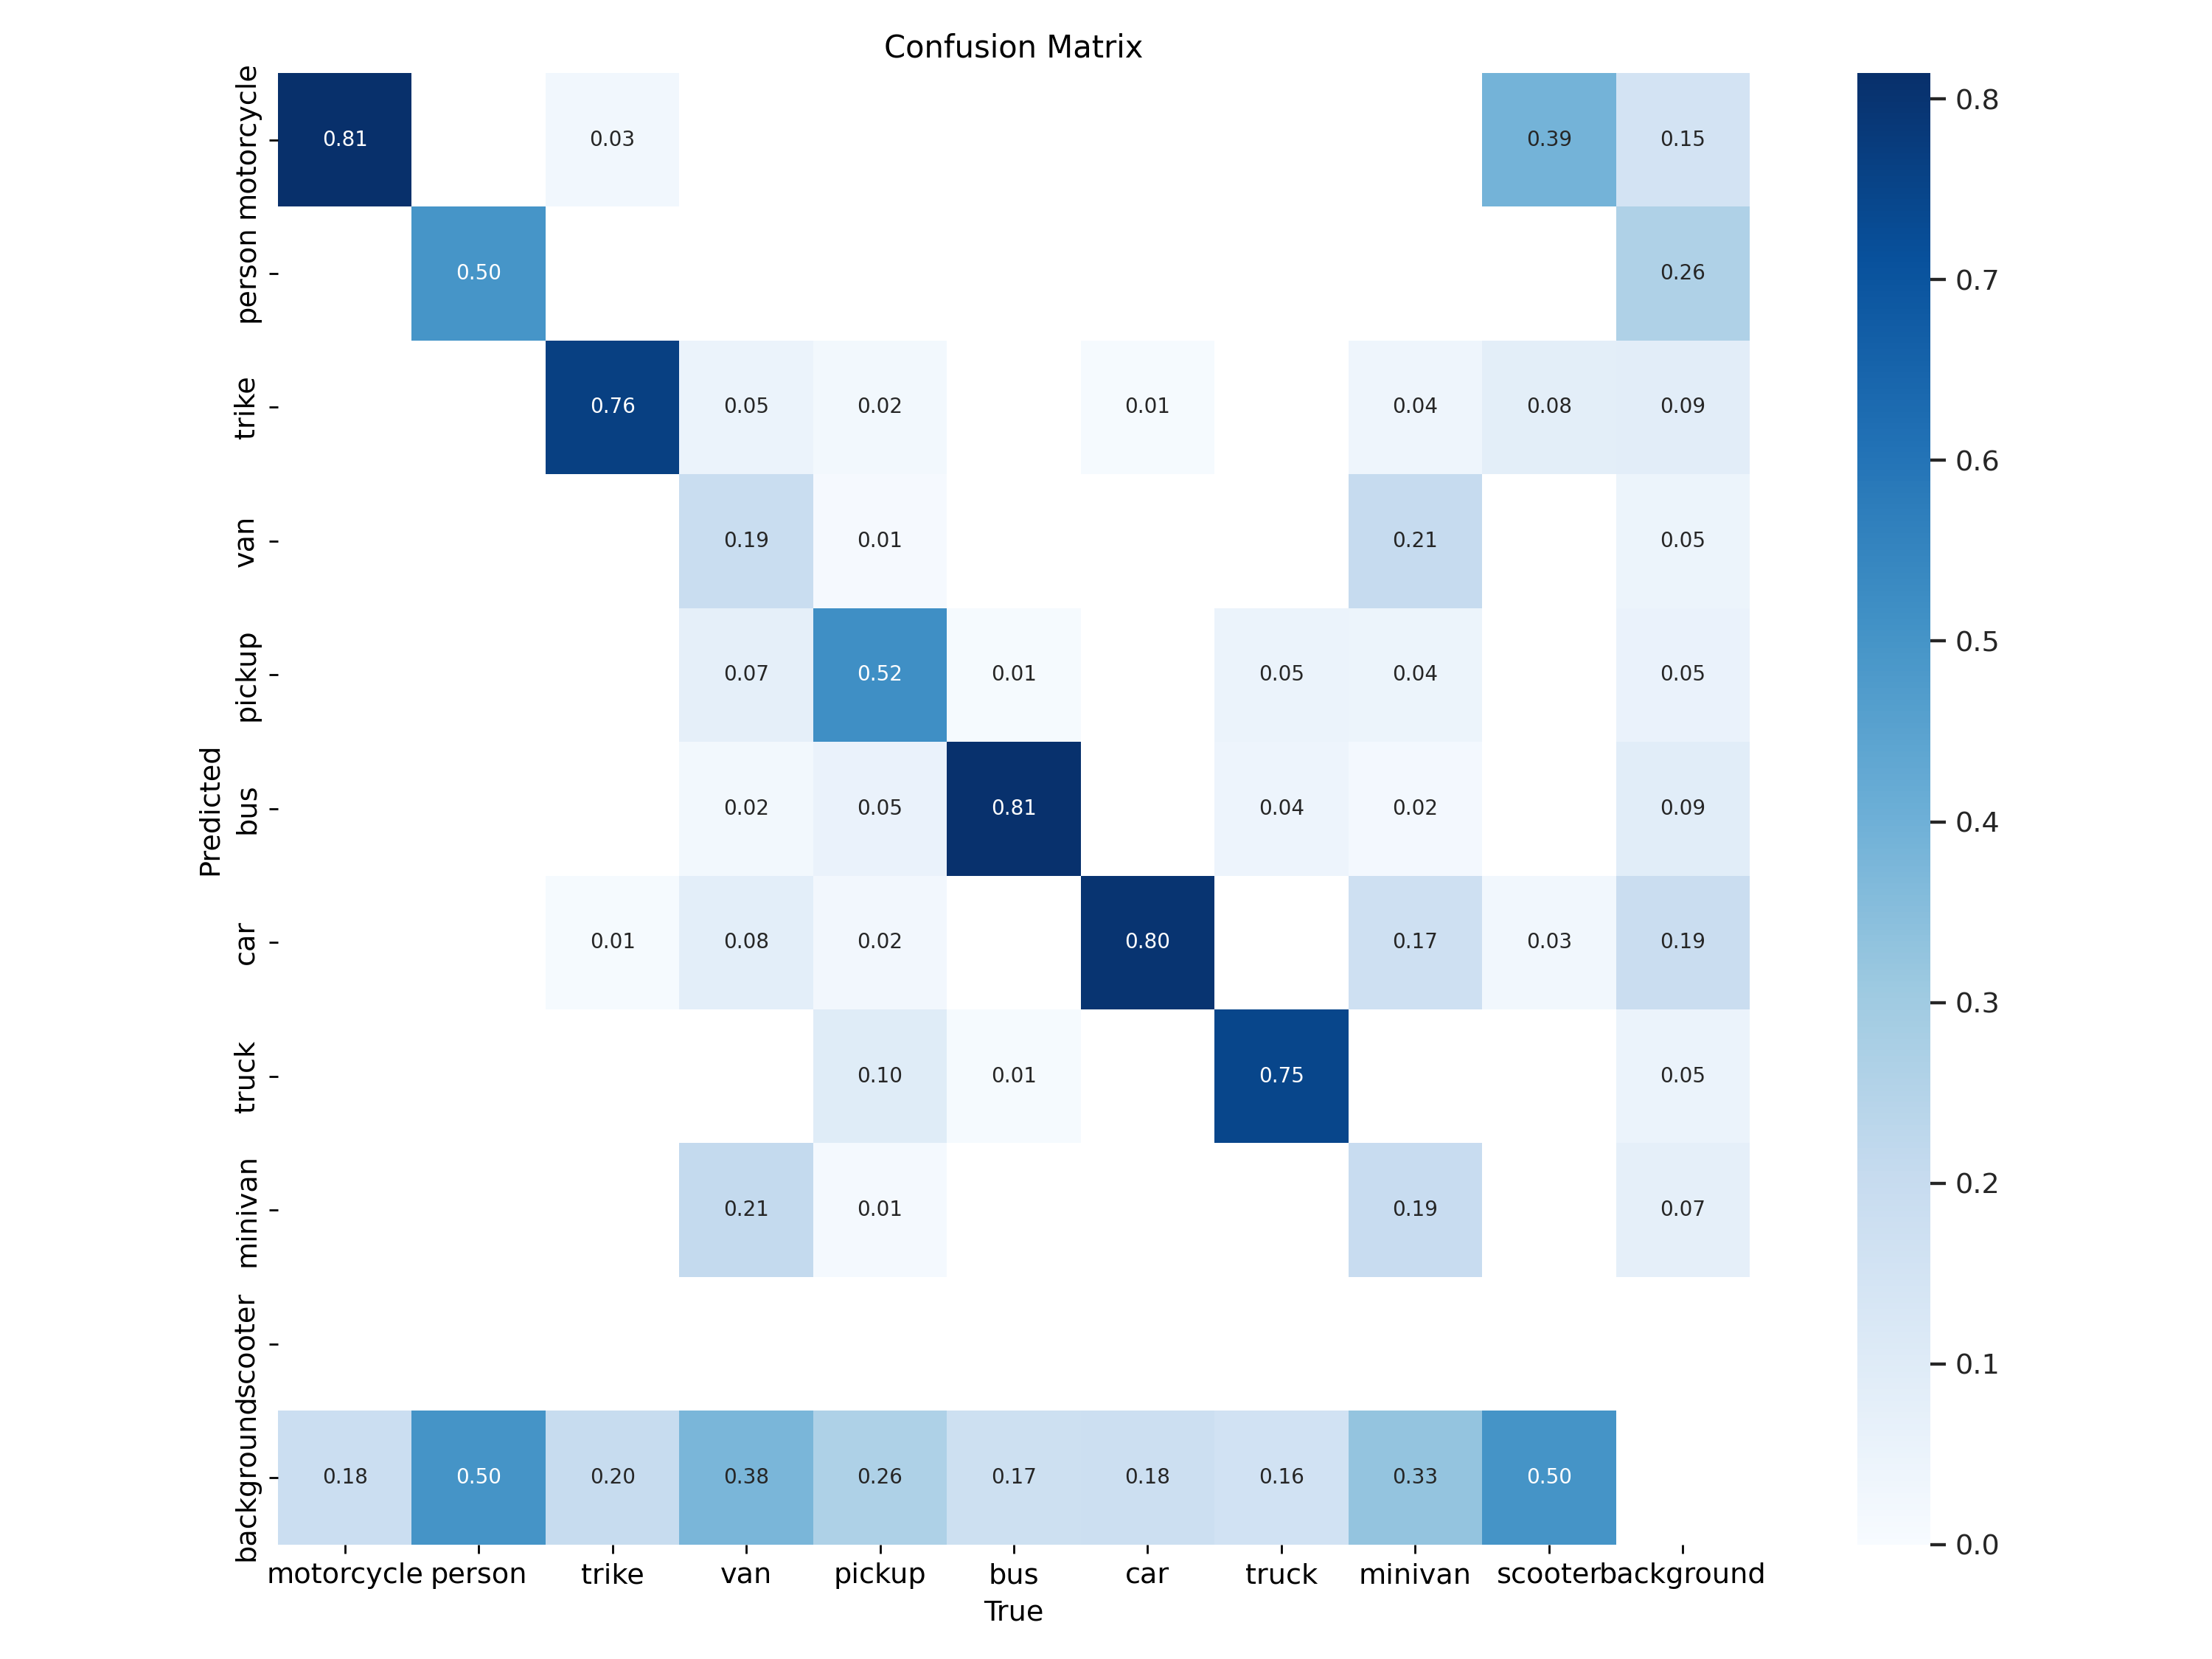
\includegraphics[width=1\columnwidth]{Figures/dataset_a/a_confusion_matrix.png}
			\caption{Dataset A: Confusion Matrix of YOLOv5 model}
			\label{fig:ukDatasetYolov5LargeWeight}
		\end{figure}

		\begin{figure}[hb]
			\centering
			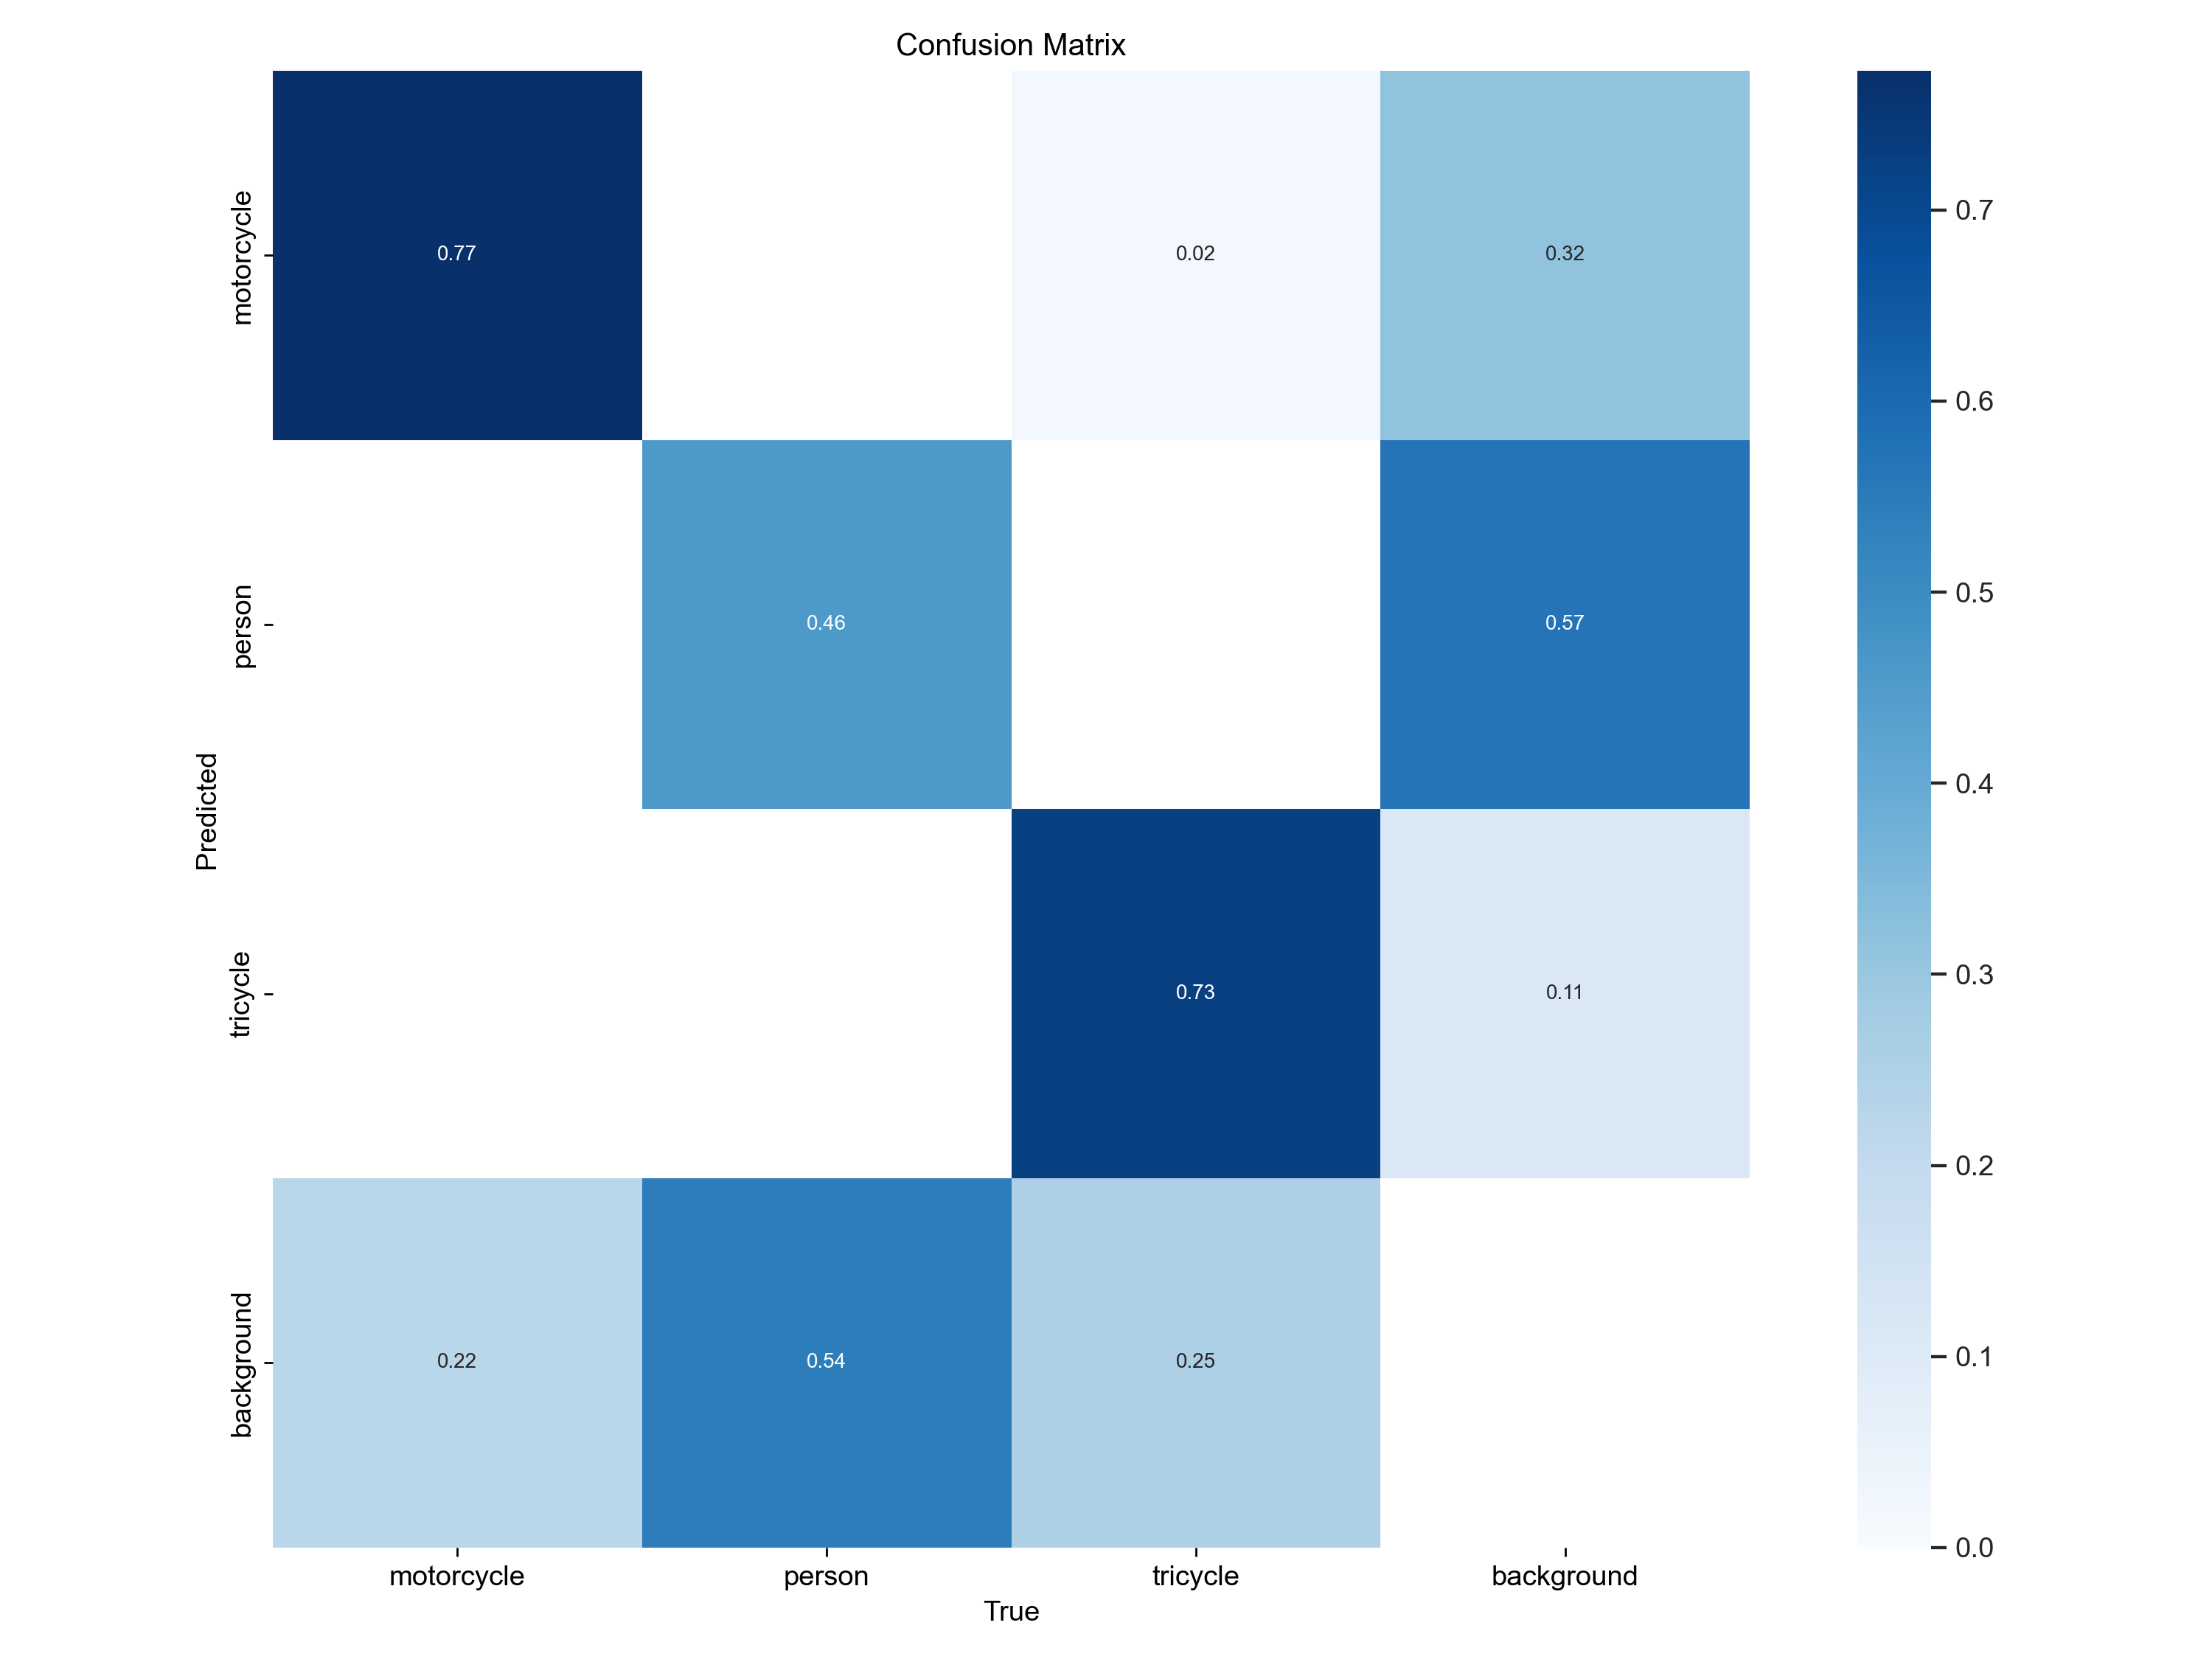
\includegraphics[width=0.95\columnwidth]{Figures/dataset_b/b_confusion_matrix.png}
			\caption{Dataset B: Confusion Matrix of YOLOv5 model}
			\label{fig:mtpDatasetYolov5LargeWeight}
		\end{figure}

		\begin{figure}[hb]
			\centering
			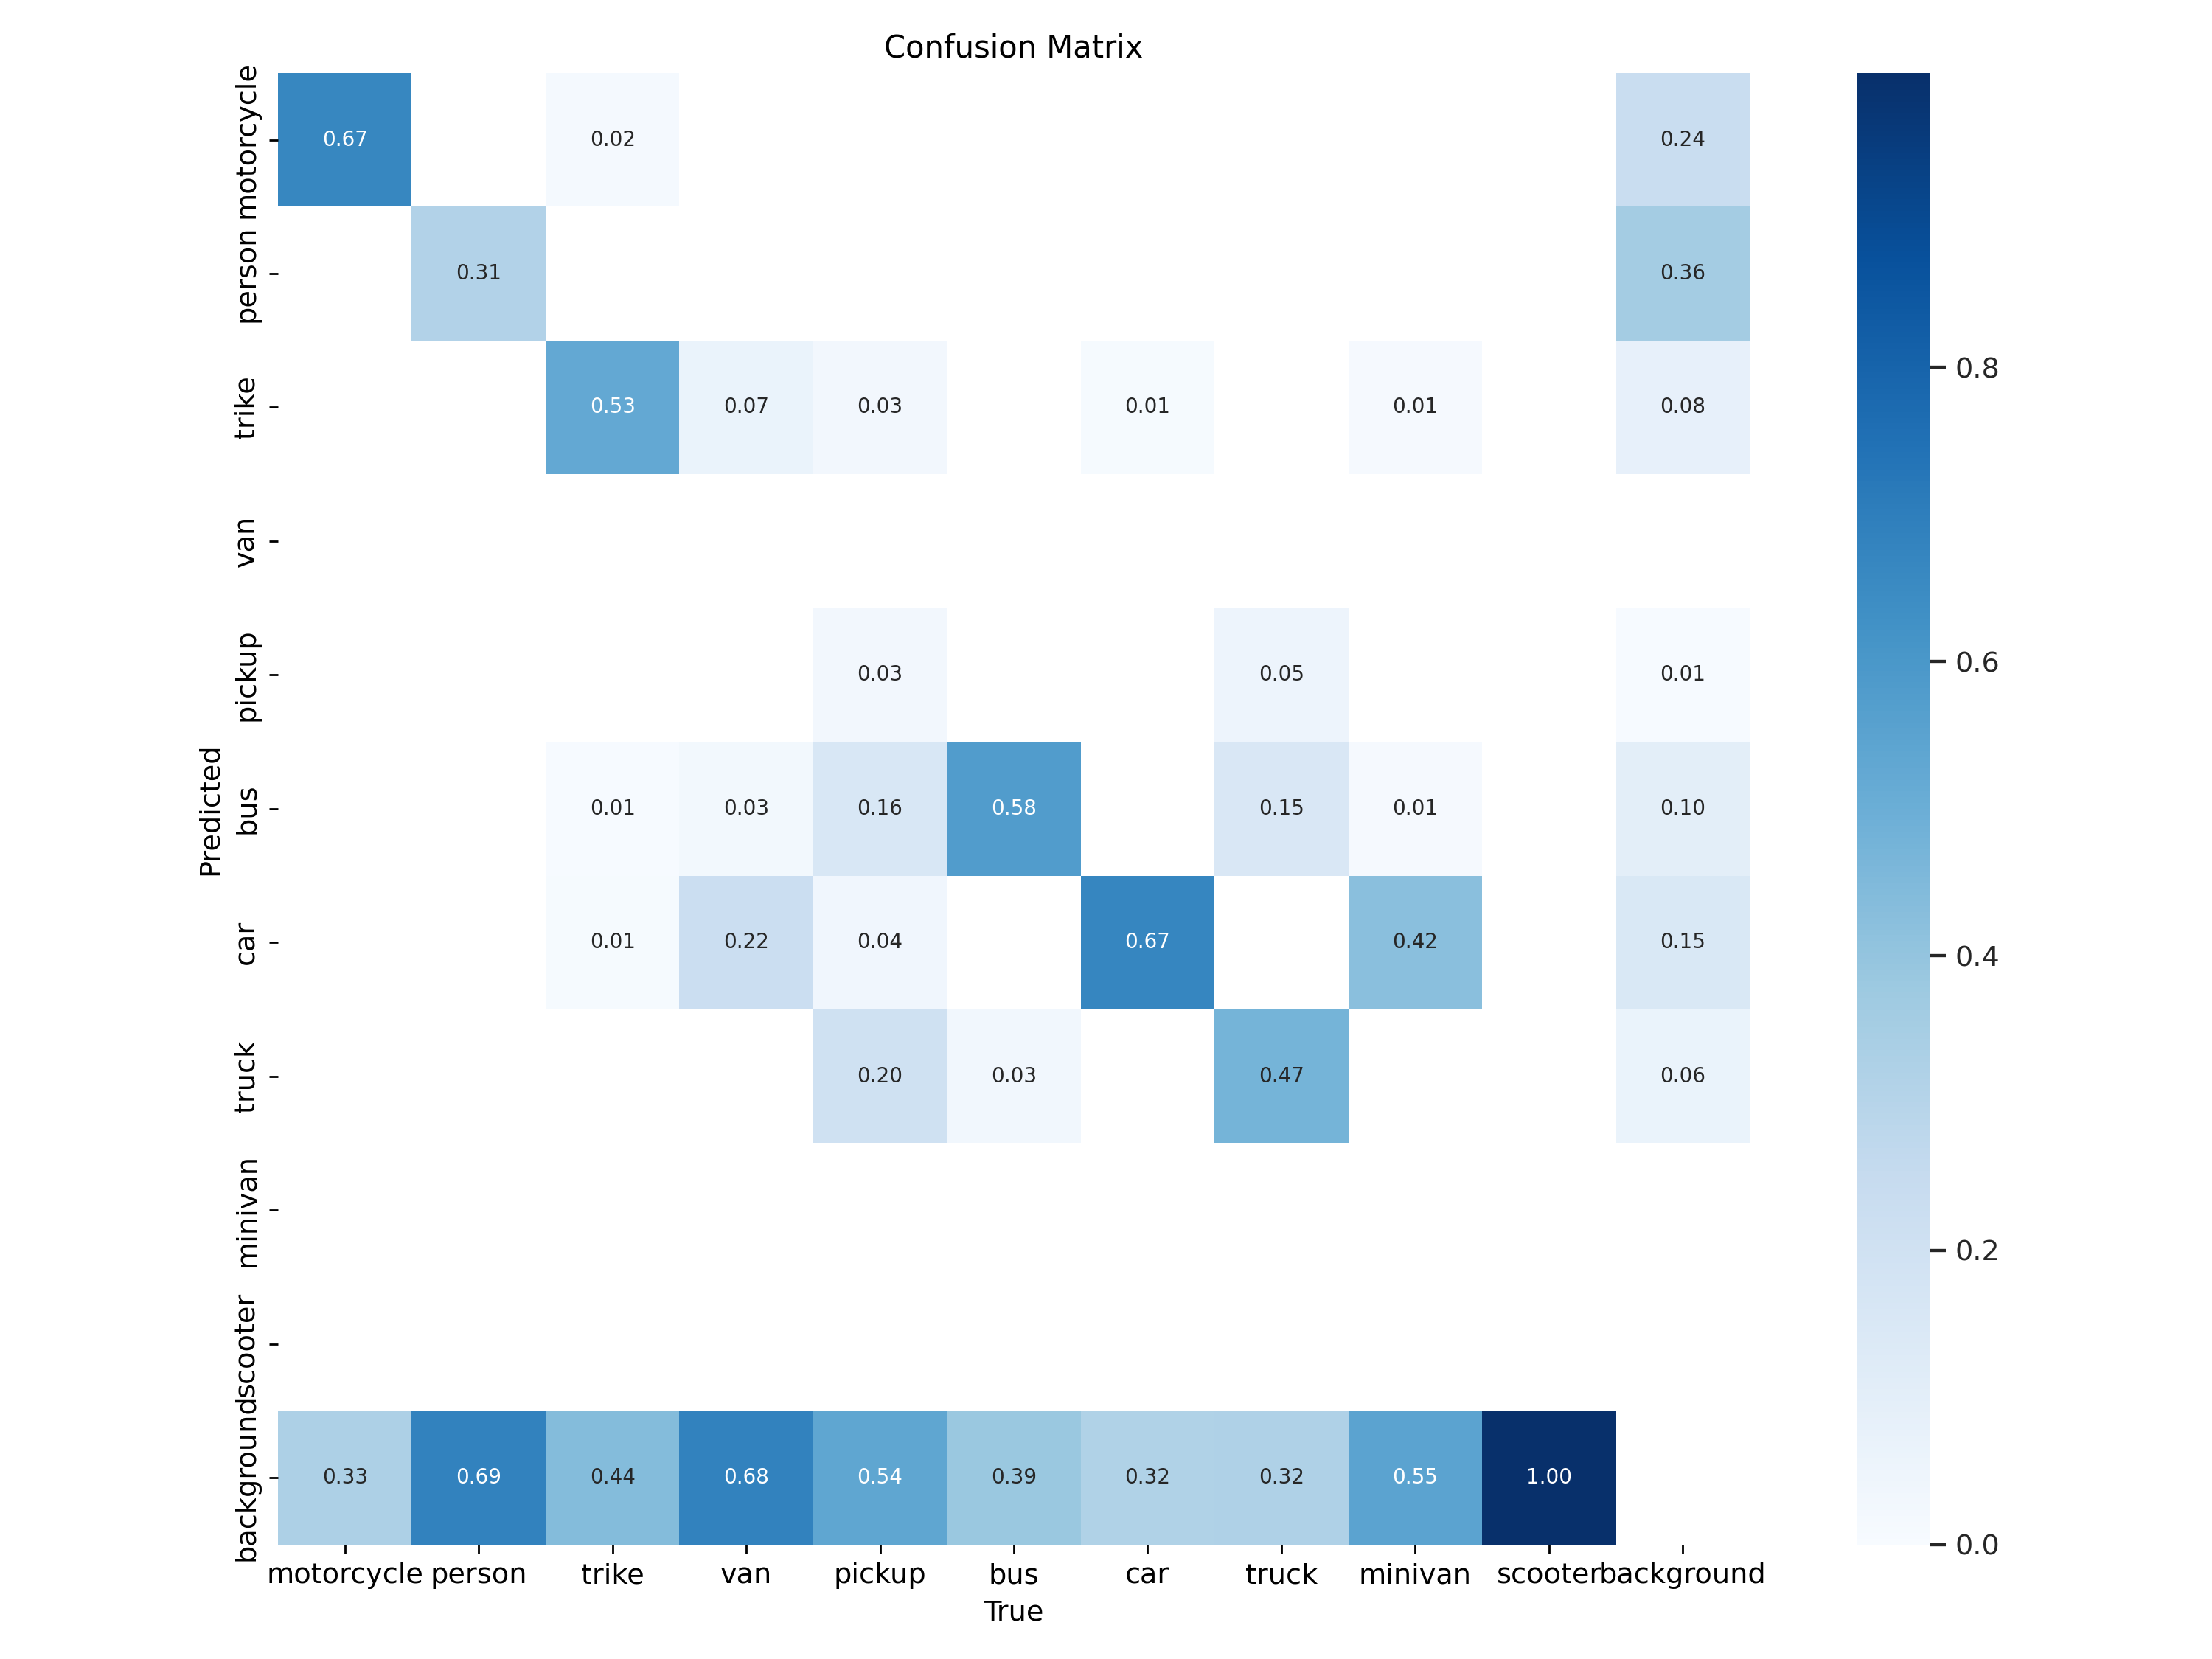
\includegraphics[width=0.95\columnwidth]{Figures/dataset_c/confusion_matrix.png}
			\caption{Dataset C: Confusion Matrix of YOLOv5 model}
			\label{fig:ntDatasetYolov5MediumWeight}
		\end{figure}

	\clearpage
	\section{PR Curves}
		Figures (\ref{fig:ukDatasetYolov5LargeWeightPRCurve},~\ref{fig:mtpDatasetYolov5LargeWeightPRCurve}) show the Precision and Recall curves plotted on a graph, giving information on any performance issues with the training models. The PR curves for both models demonstrate high precision across varying levels of recall, indicative of robust performance. Although, figure~\ref{fig:ukDatasetYolov5LargeWeightPRCurve} appears to have a higher precision for the longer part of the training process, compared to figure~\ref{fig:mtpDatasetYolov5LargeWeightPRCurve}. The worst performers of the model are scooters, vans, person and minivans in precision and perform well when it comes to recall. In comparison, figure~\ref{fig:mtpDatasetYolov5LargeWeightPRCurve} shows a similar illustration. According to the key of figure~\ref{fig:ukDatasetYolov5LargeWeightPRCurve}, motorcycles had a higher precision peak at 77.5\% compared to figure~\ref{fig:mtpDatasetYolov5LargeWeightPRCurve}. The model architecture performs well when training the given dataset scenarios. Perhaps larger weights could increase the precision and recall curve during training. It is worth mentioning that the preparation of the datasets functions well during the training process, and no underlying problems are showing, especially for motorcycle data. `Dataset C', fig~\ref{fig:ntDatasetYolov5MediumWeight} appears to have a curve to `Dataset B' when looking into the `motorcycle' classification. However, the overall Precision-to-Recall is poor and suggests that the model struggled in identifying the overall classifications.

		\begin{figure}[ht]
			\floatsetup{valign=t, heightadjust=object}
			\begin{floatrow}
				\ffigbox[0.80\linewidth]
				{
					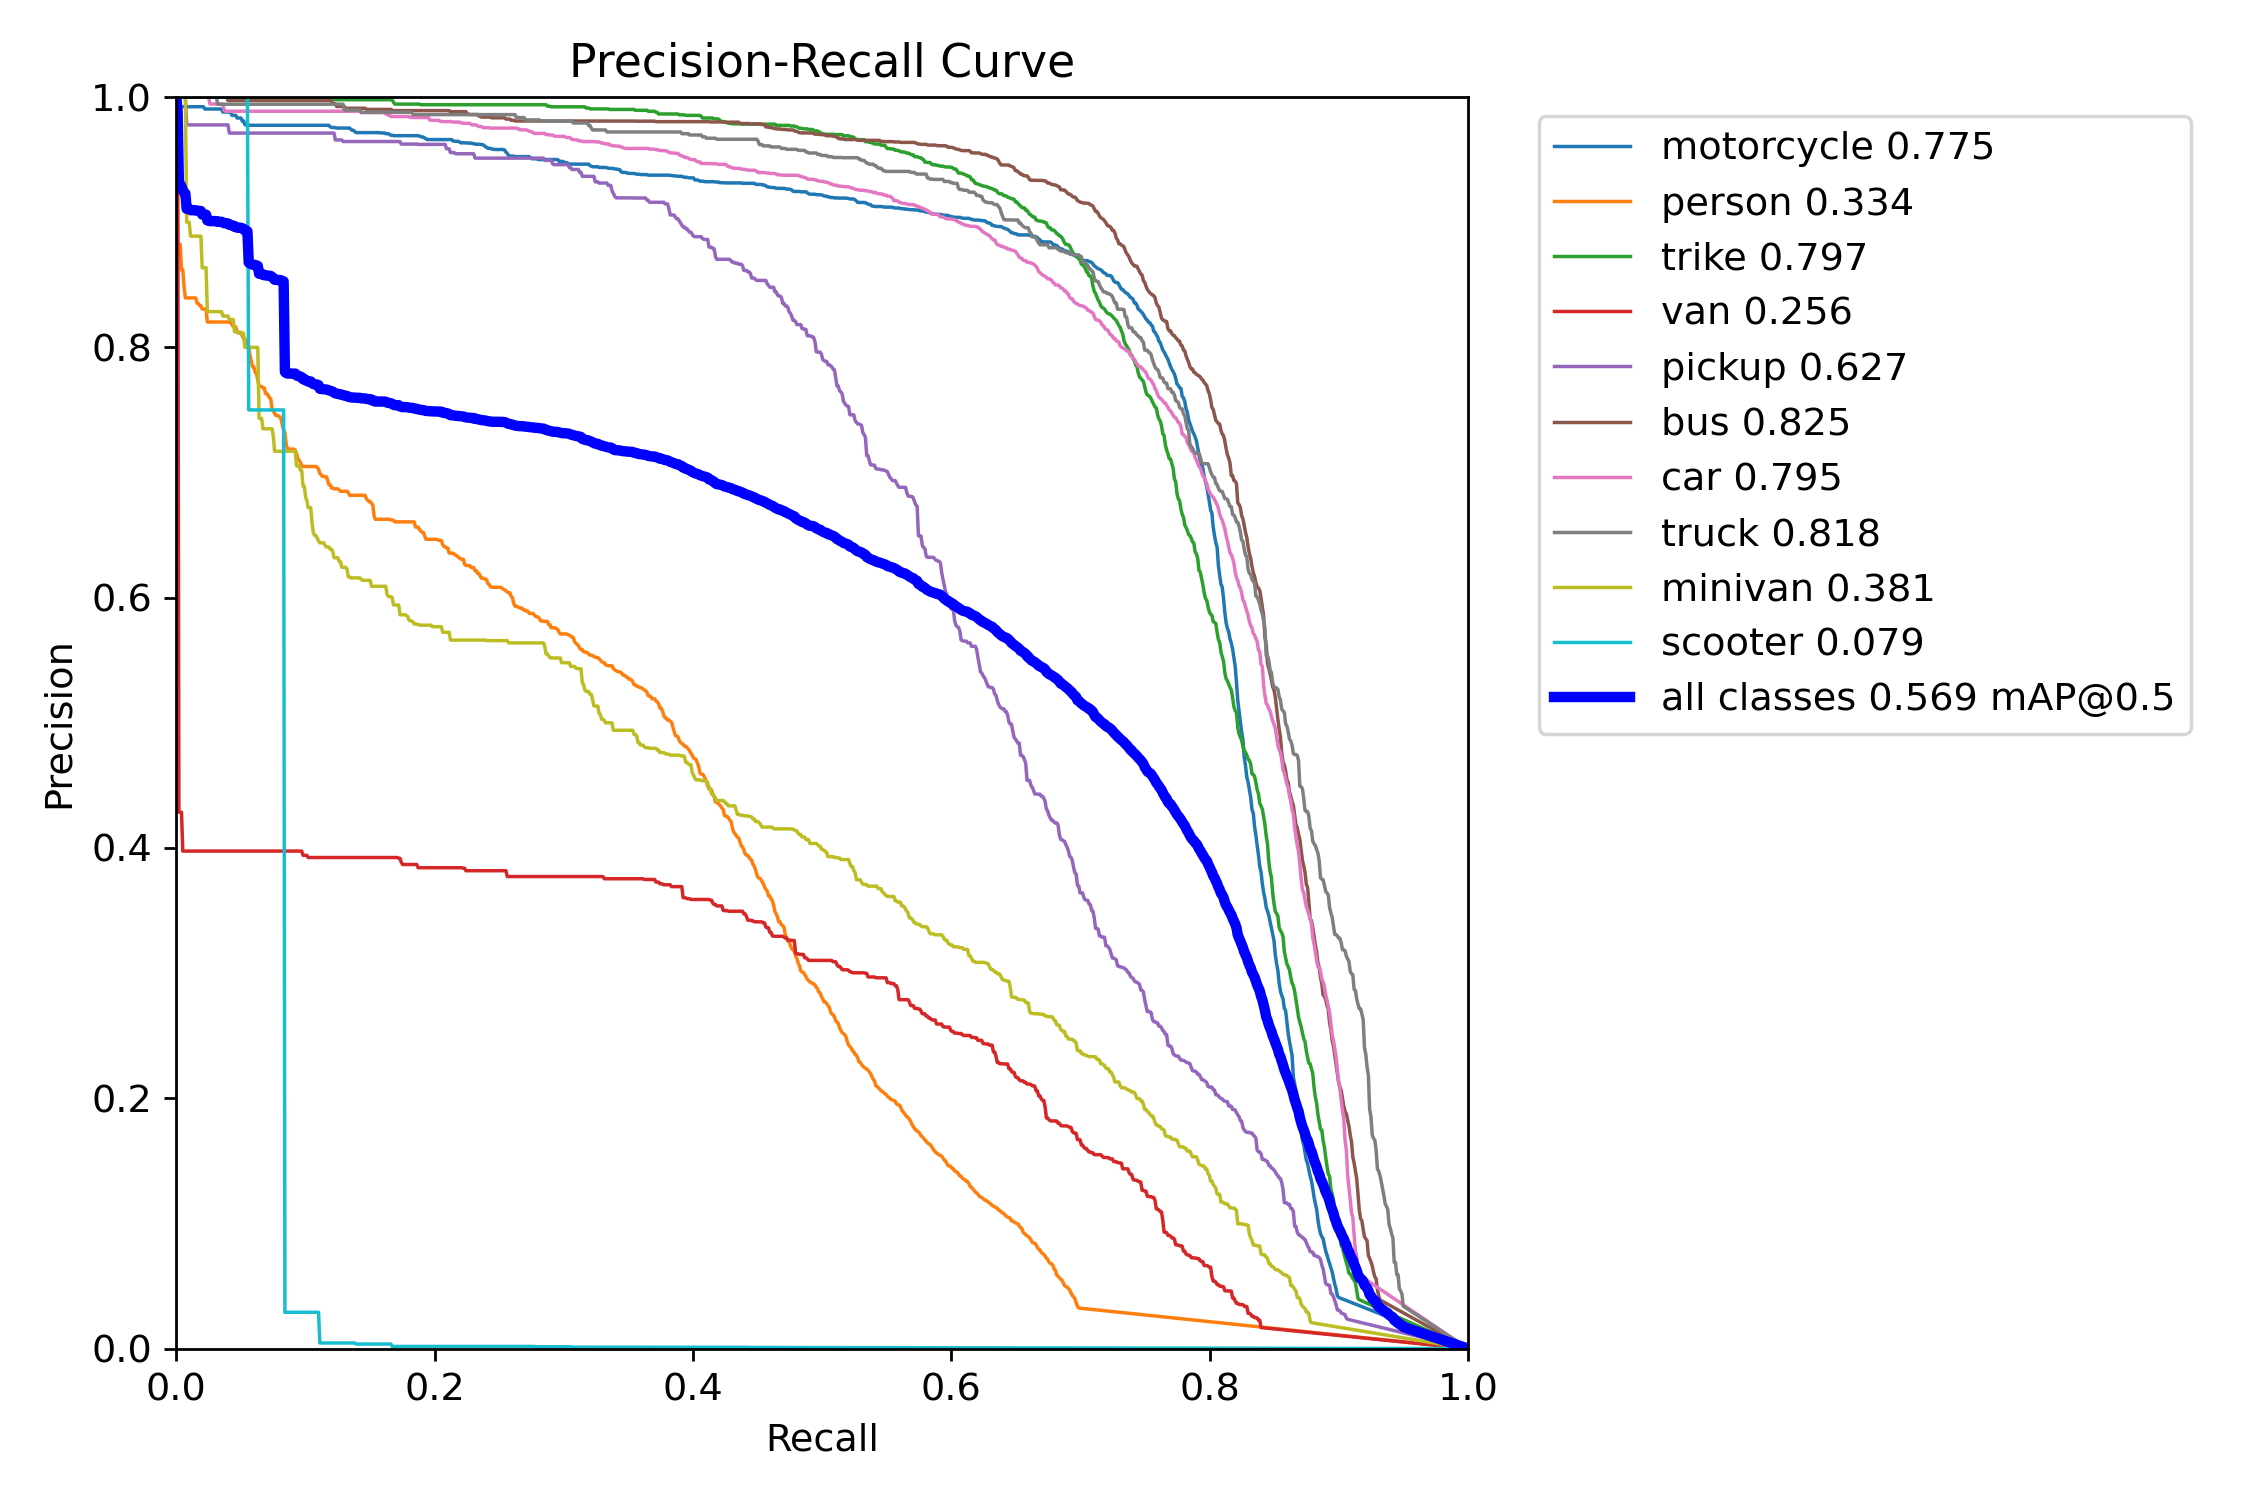
\includegraphics[width=1\linewidth]{Figures/dataset_a/PR_curve.png}
				}
				{
					\caption{Dataset A: Performance and Recall Curve of YOLOv5 model}
					\label{fig:ukDatasetYolov5LargeWeightPRCurve}
				}
			
				\ffigbox[0.80\linewidth]
				{
					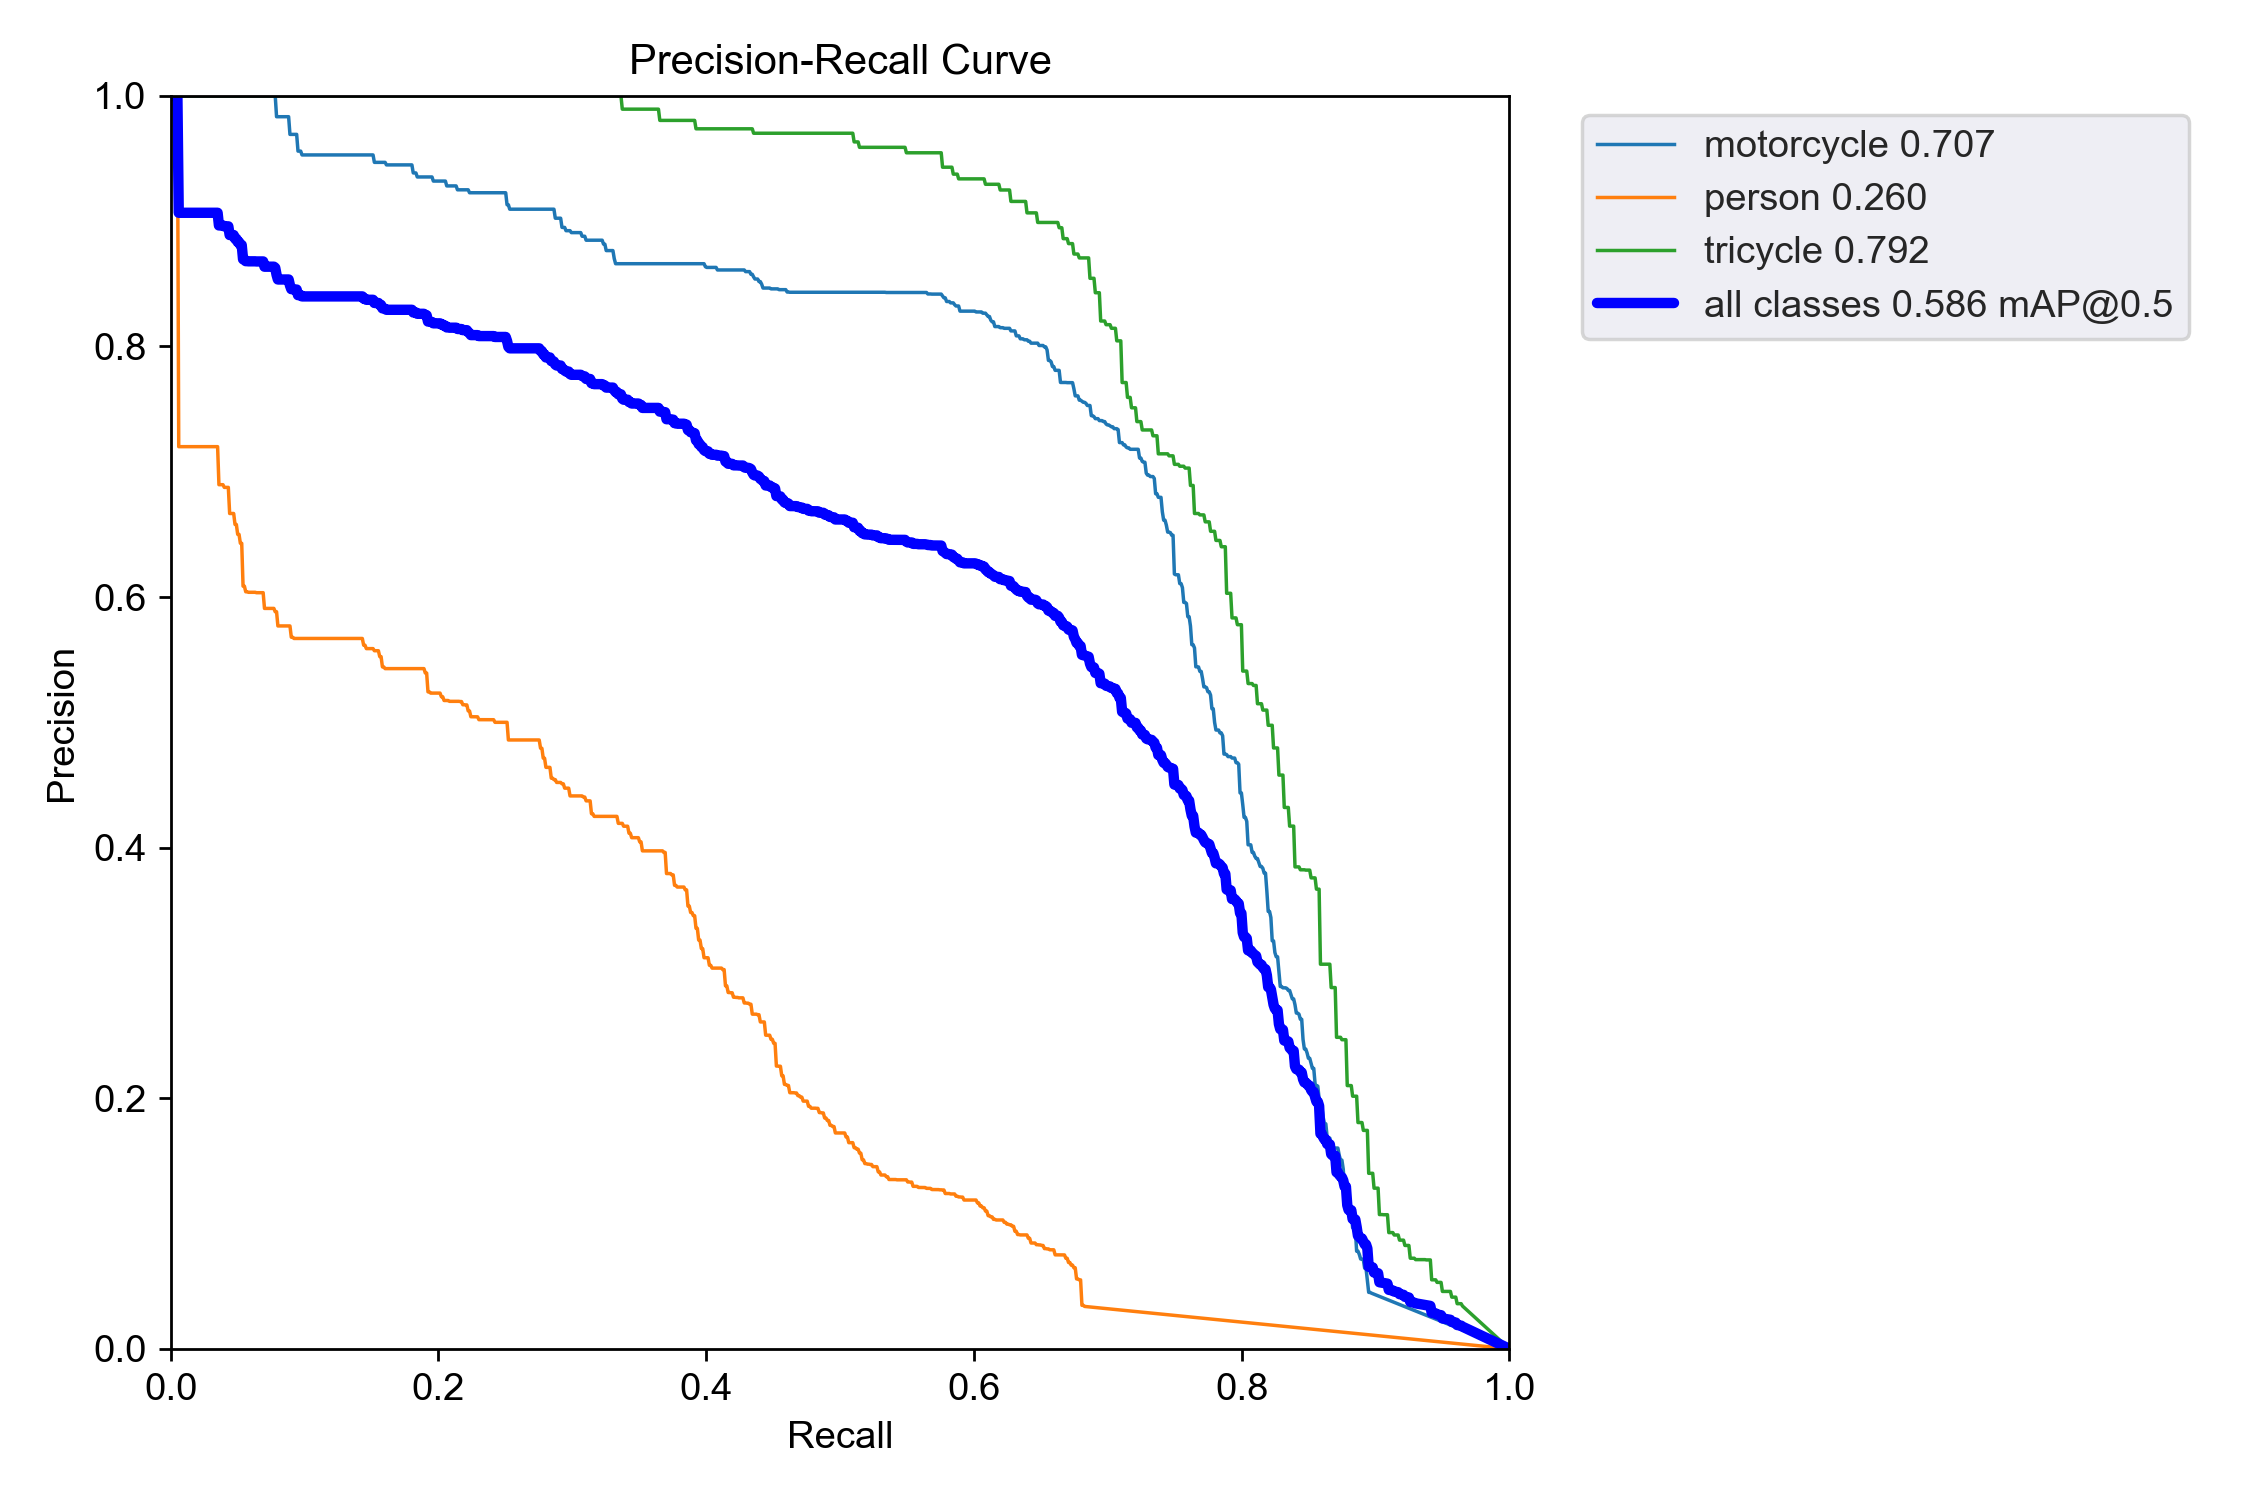
\includegraphics[width=1\linewidth]{Figures/dataset_b/PR_curve.png}
				}
				{
					\caption{Dataset B: Performance and Recall of YOLOv5 model}
					\label{fig:mtpDatasetYolov5LargeWeightPRCurve}
				}
			\end{floatrow}
		\end{figure}

		\begin{figure}[hb]
			\centering
			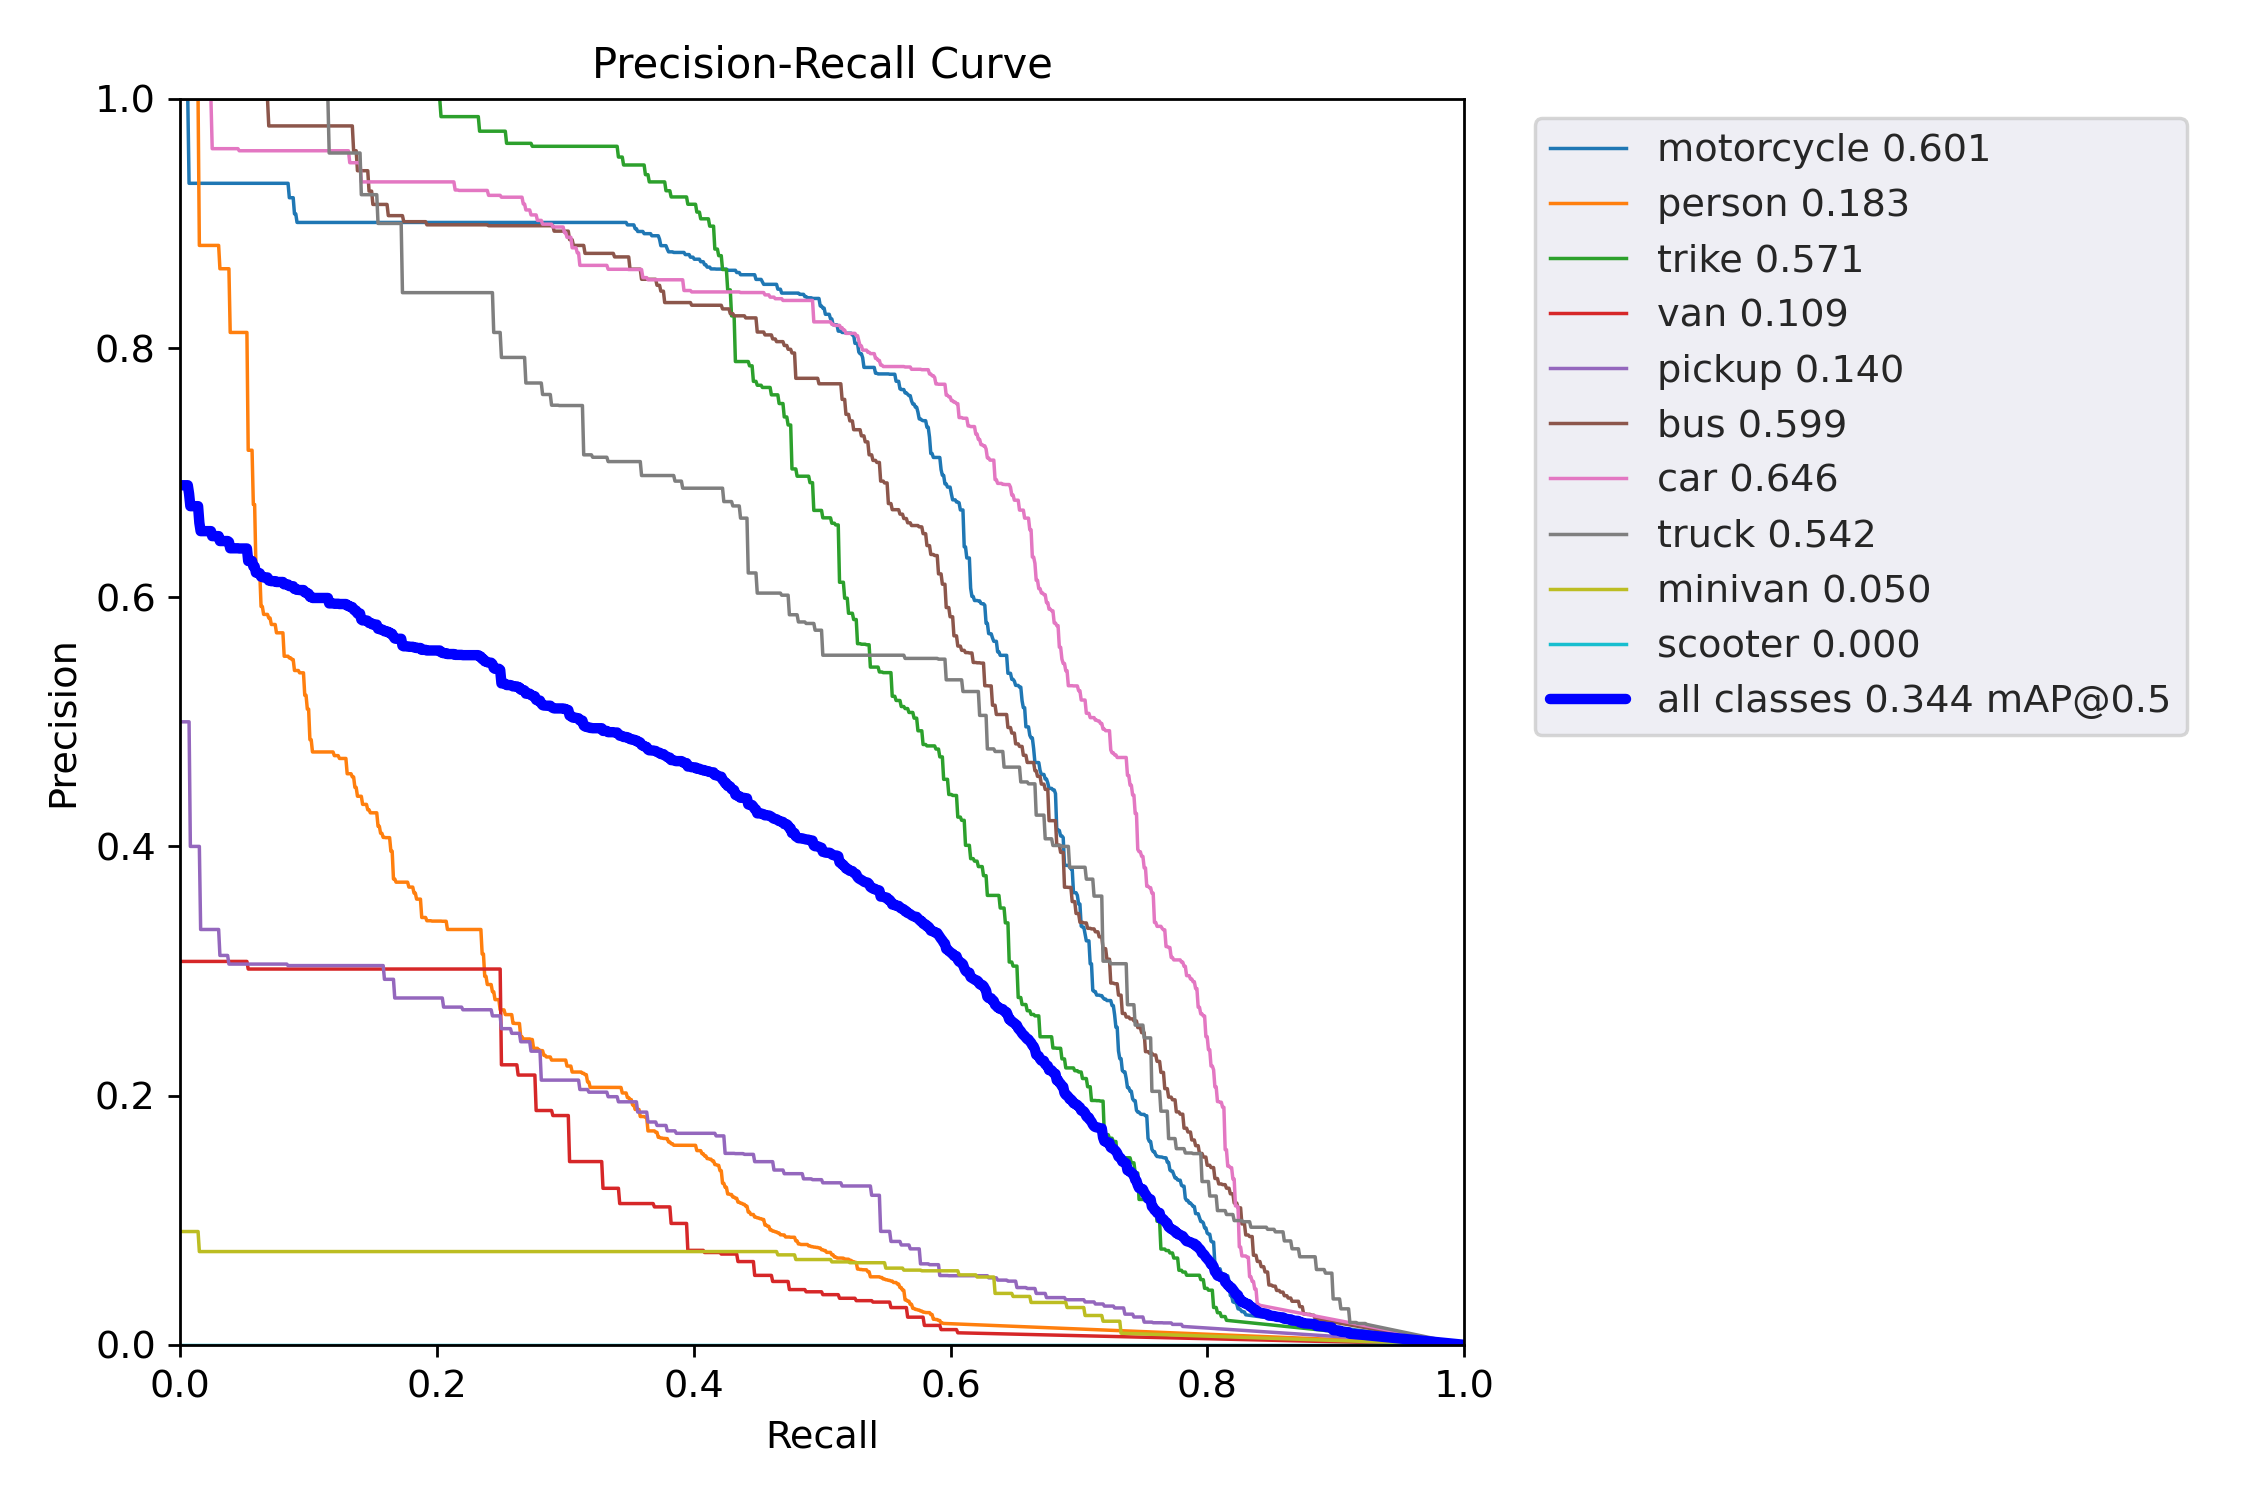
\includegraphics[width=.50\columnwidth]{Figures/dataset_c/PR_curve.png}
			\caption{Dataset C: Performance and Recall of YOLOv5 model}
			\label{fig:ntDatasetYolov5MediumWeightPRCurve}
		\end{figure}

	\clearpage
	\section{F1 Confidence Curves}
		Figures (\ref{fig:ukDatasetYolov5LargeWeightF1Curve},~\ref{fig:mtpDatasetYolov5LargeWeightF1Curve}) showcase the `Dataset A' and `Dataset B' datasets on an F1-Confidence curve. The F1-Score is calculated with the following equations:-
		\begin{center}
			\textbf{\textit{TP:}} True Positives | \textbf{\textit{FP:}} False Positives

			\textbf{Precision:} $\mathcal{P} = \frac{\text{TP}}{\text{TP} + \text{FP}}$

			\textbf{Recall:} $\mathcal{R} = \frac{\text{TP}}{\text{TP} + \text{FN}}$
			
			\textbf{F1-Score:} $\mathcal{F\textit{1}} = \frac{2 \times \mathcal{P} \times \mathcal{R}}{\mathcal{P} + \mathcal{R}}$
		\end{center}

		The daylight learning curves of the model are healthy and optimal. The F1-Score of fig~\ref{fig:ukDatasetYolov5LargeWeightF1Curve} performs better for motorcycles, compared to fig~\ref{fig:mtpDatasetYolov5LargeWeightF1Curve} achieving a higher F1-Score and confidence level. The night-time learning curves show a lower F1-Score to confidence level, shown in fig~\ref{fig:ntDatasetYolov5MediumWeightF1Curve}, which is terrible compared to the daylight dataset models learning curves. The low F1-Score shows a bigger Recall.

		\begin{figure}[ht]
			\floatsetup{valign=t, heightadjust=object}
			\begin{floatrow}
				\ffigbox[0.85\linewidth]
				{
					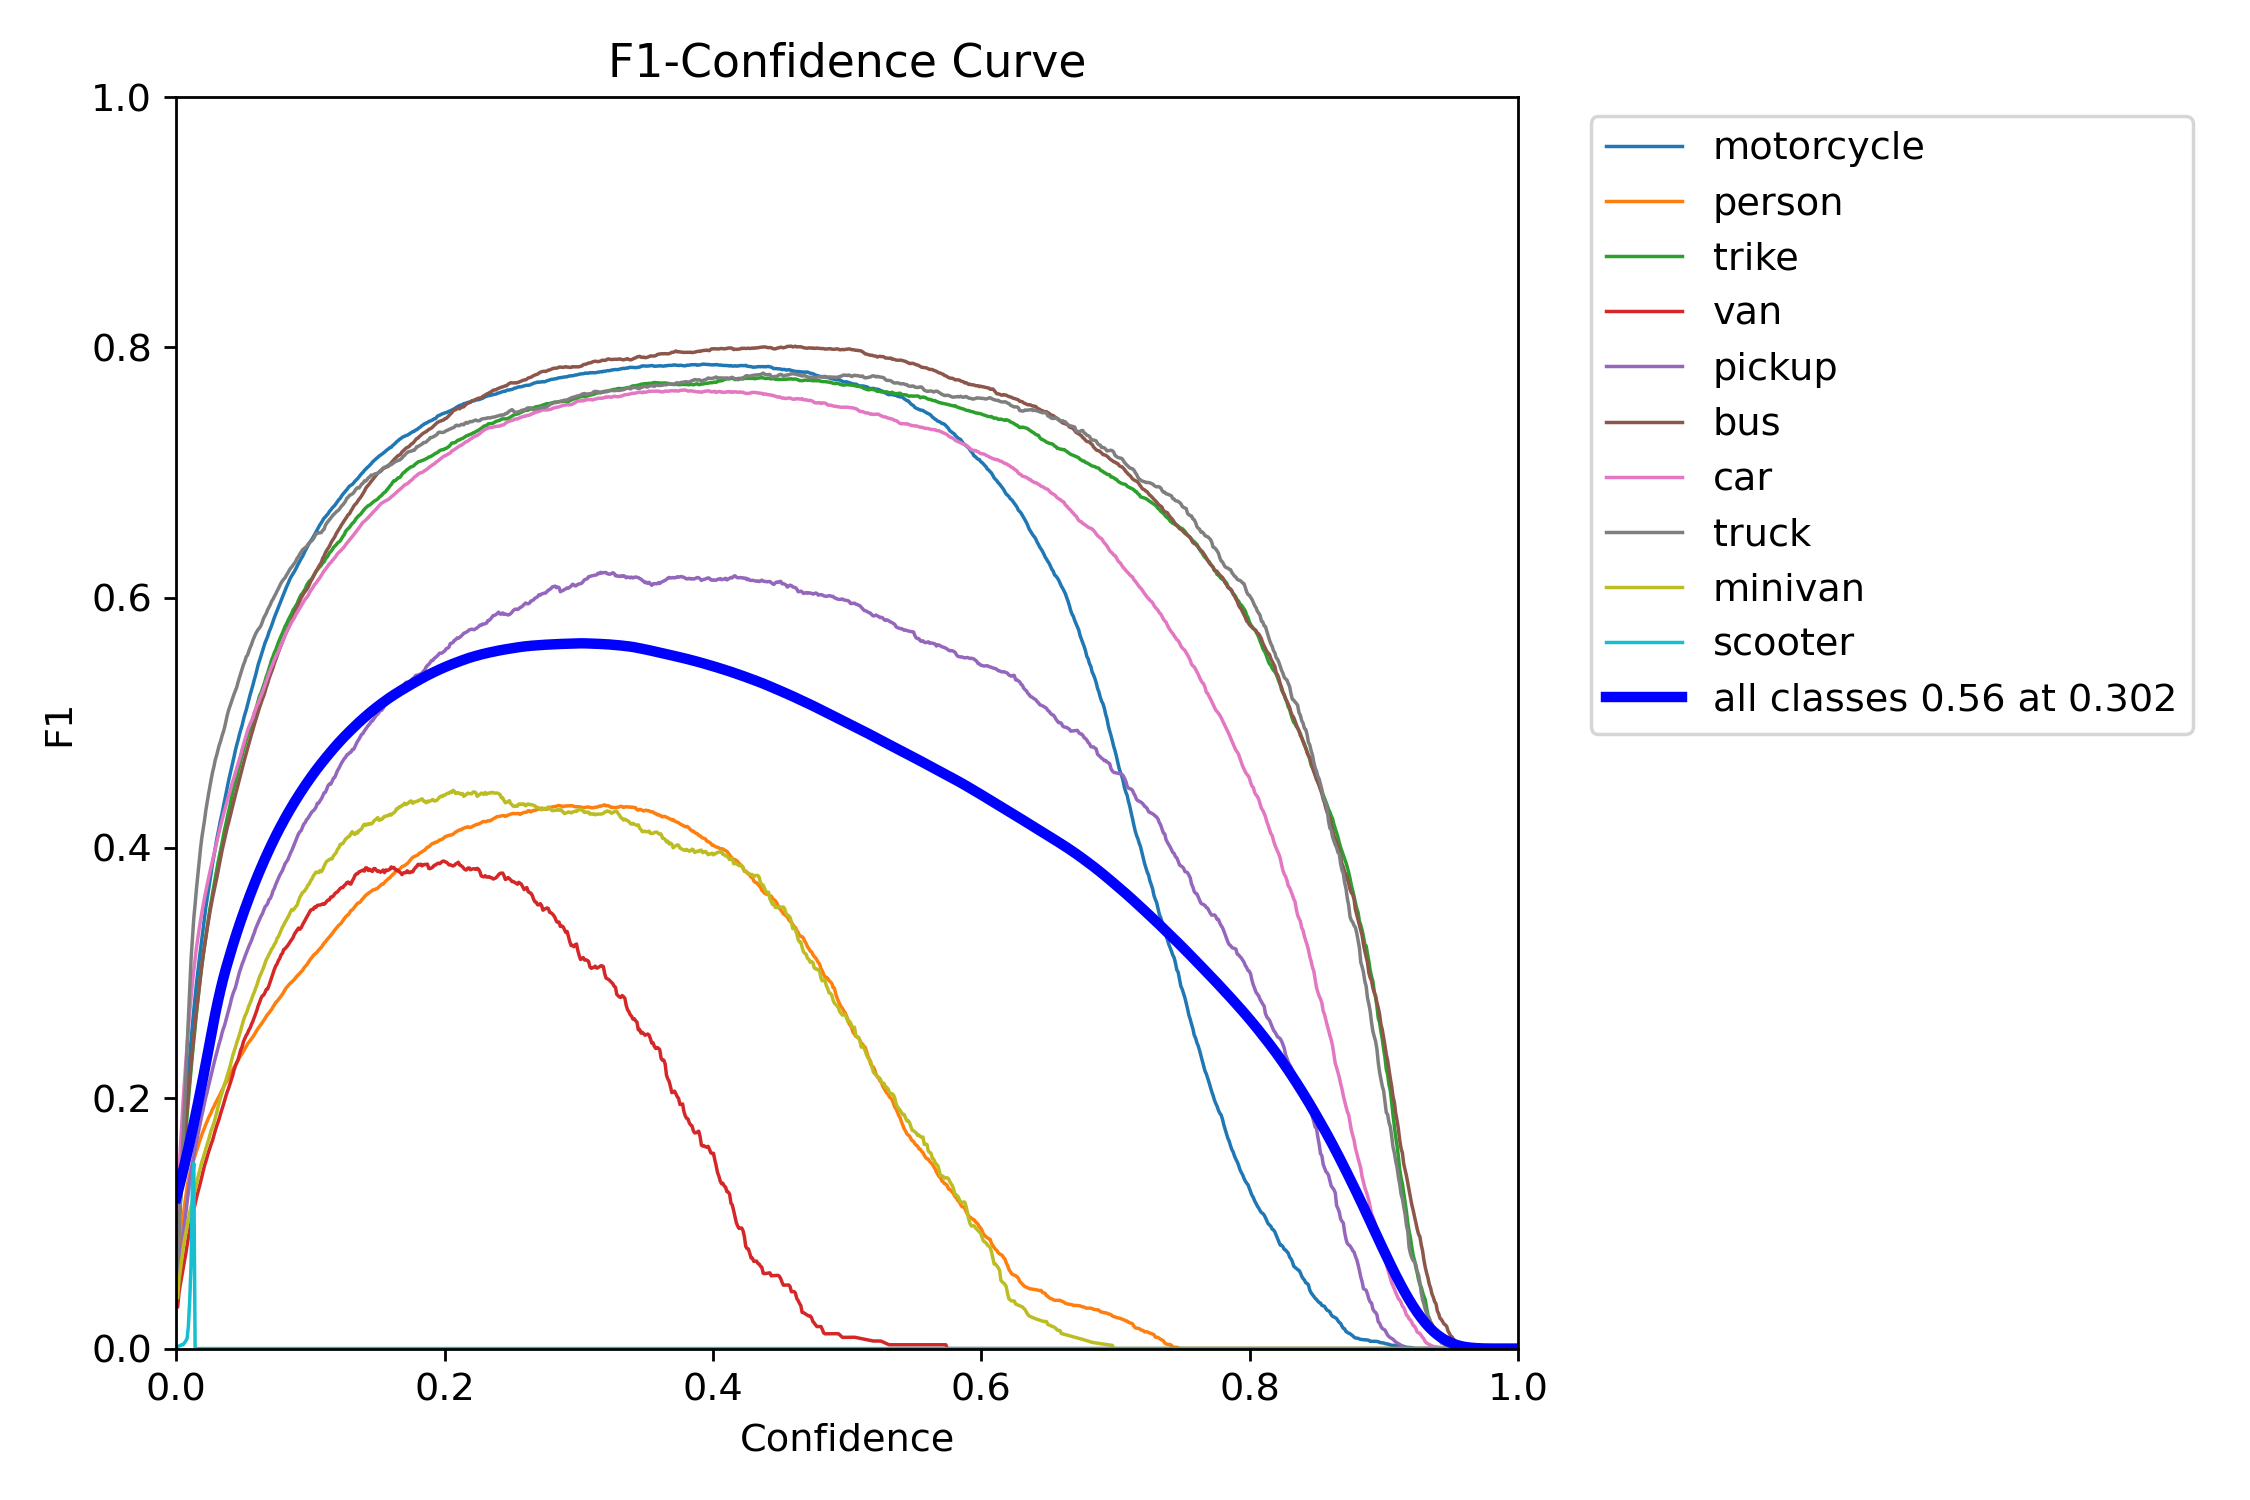
\includegraphics[width=1\linewidth]{Figures/dataset_a/F1_curve.png}
				}
				{
					\caption{Dataset A: F1 Confidence Curve of YOLOv5 model}
					\label{fig:ukDatasetYolov5LargeWeightF1Curve}
				}
			
				\ffigbox[0.85\linewidth]
				{
					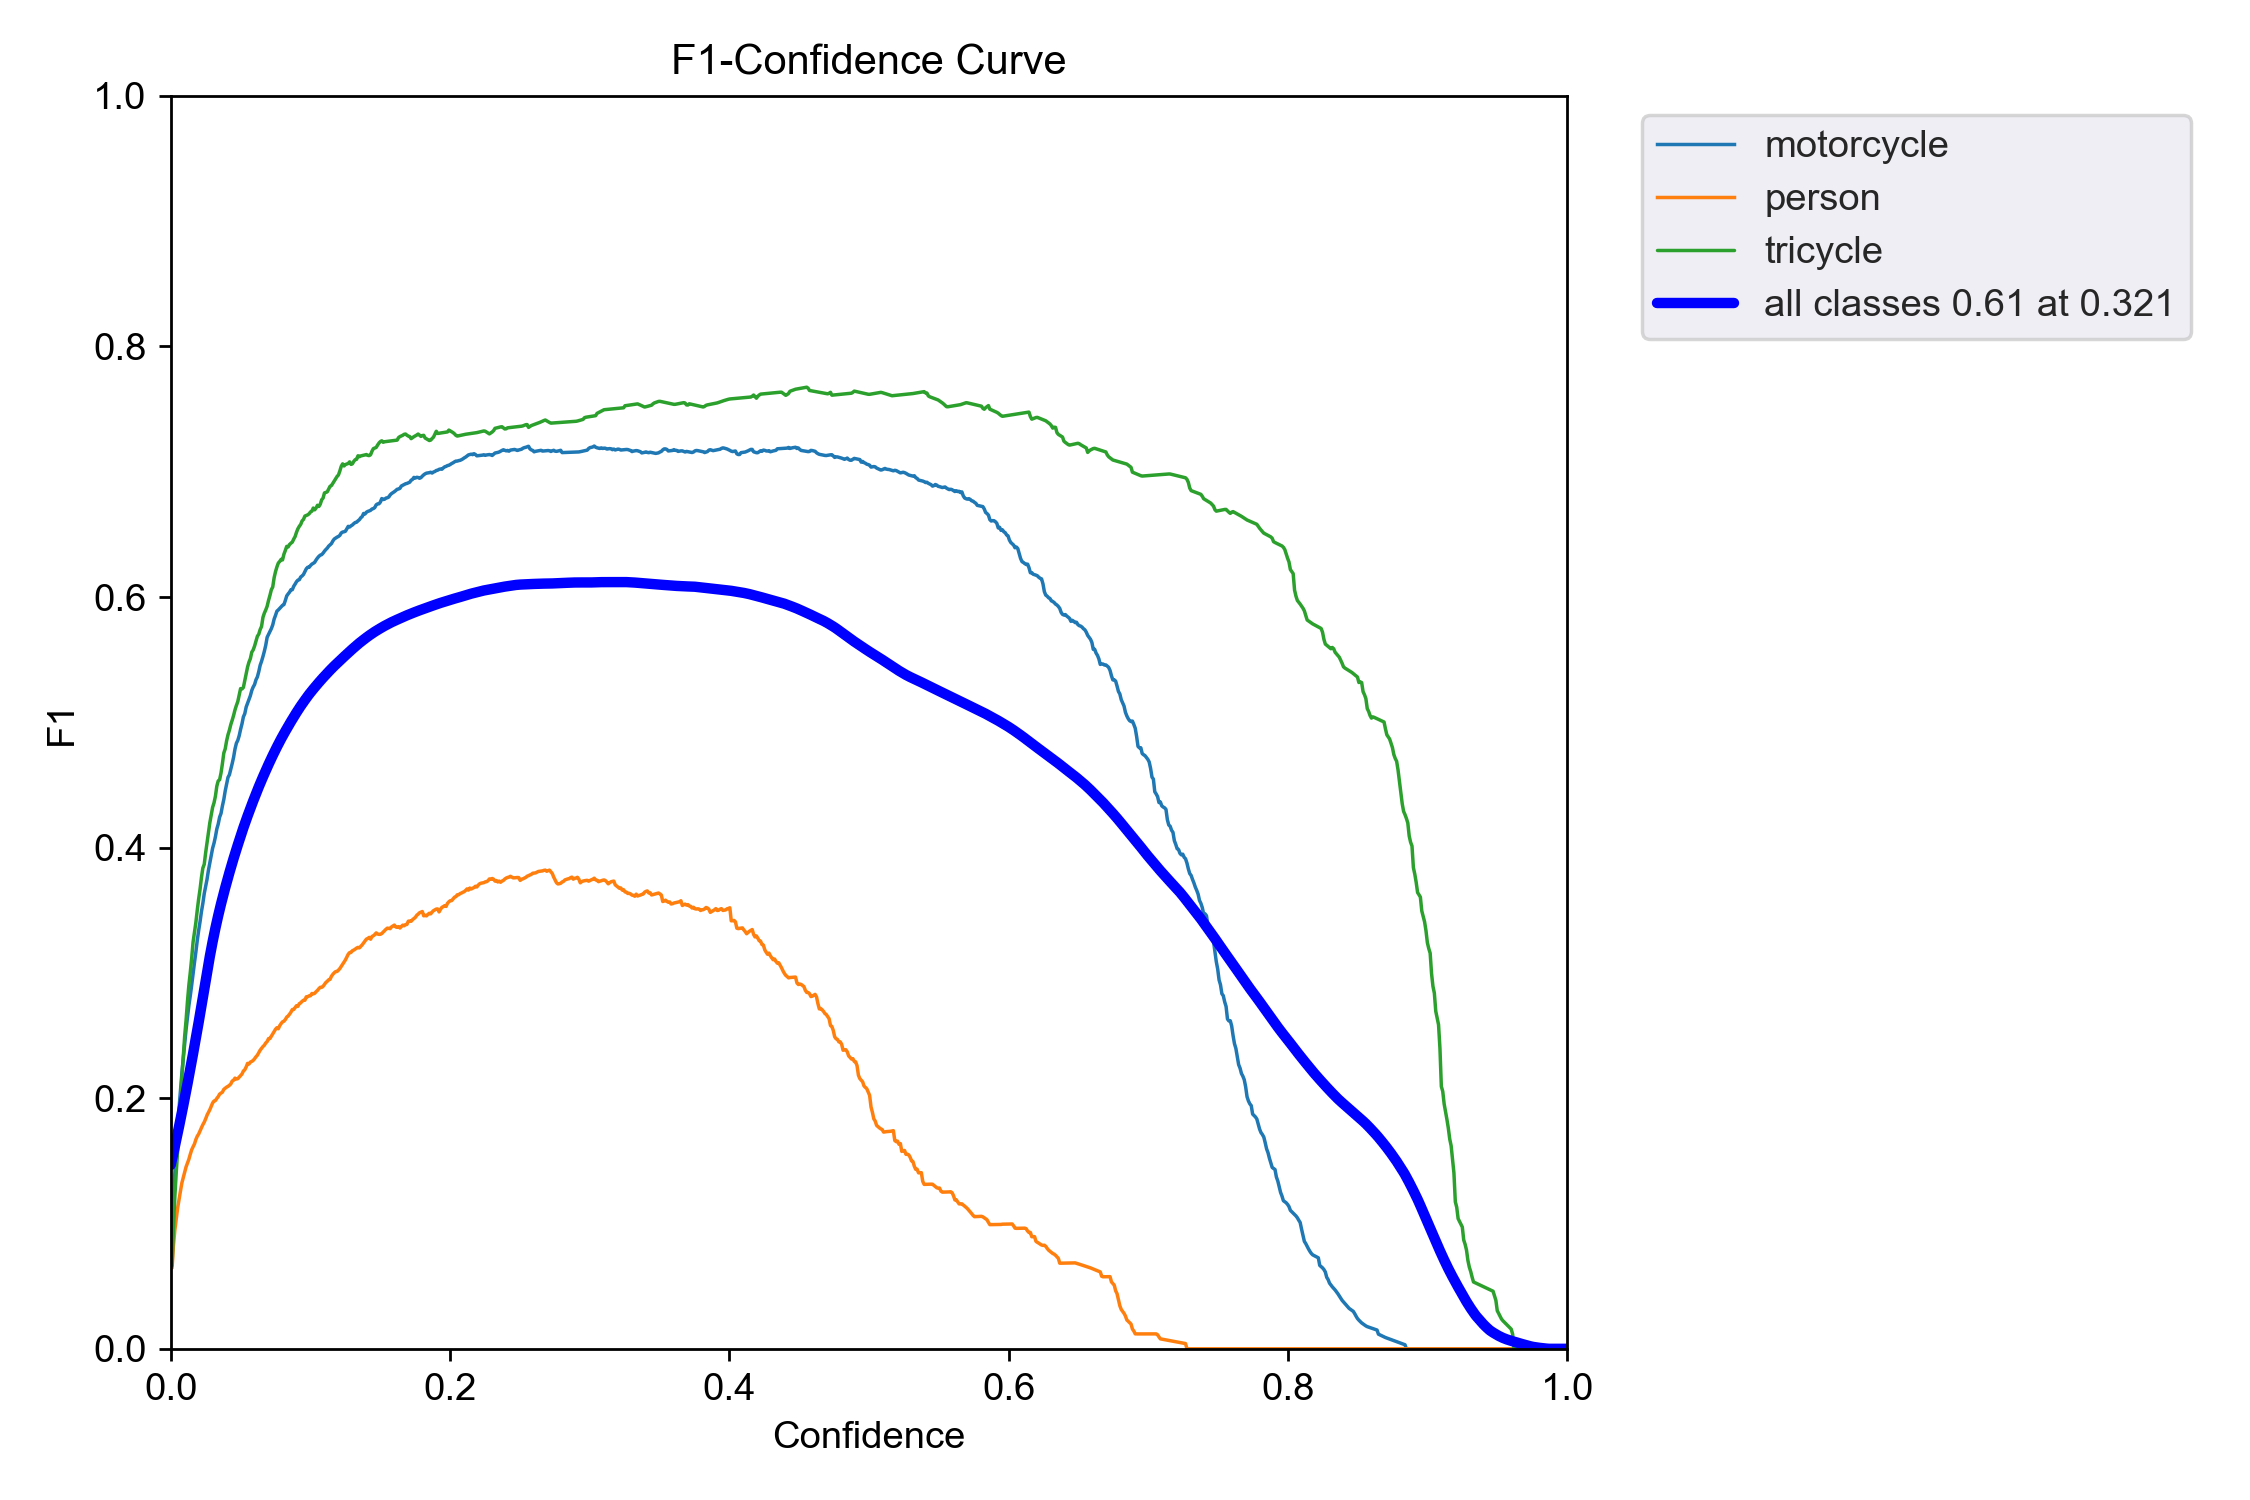
\includegraphics[width=1\linewidth]{Figures/dataset_b/F1_curve.png}
				}
				{
					\caption{Dataset B: F1 Confidence Curve of YOLOv5 model}
					\label{fig:mtpDatasetYolov5LargeWeightF1Curve}
				}
			\end{floatrow}
		\end{figure}

		\begin{figure}[hb]
			\centering
			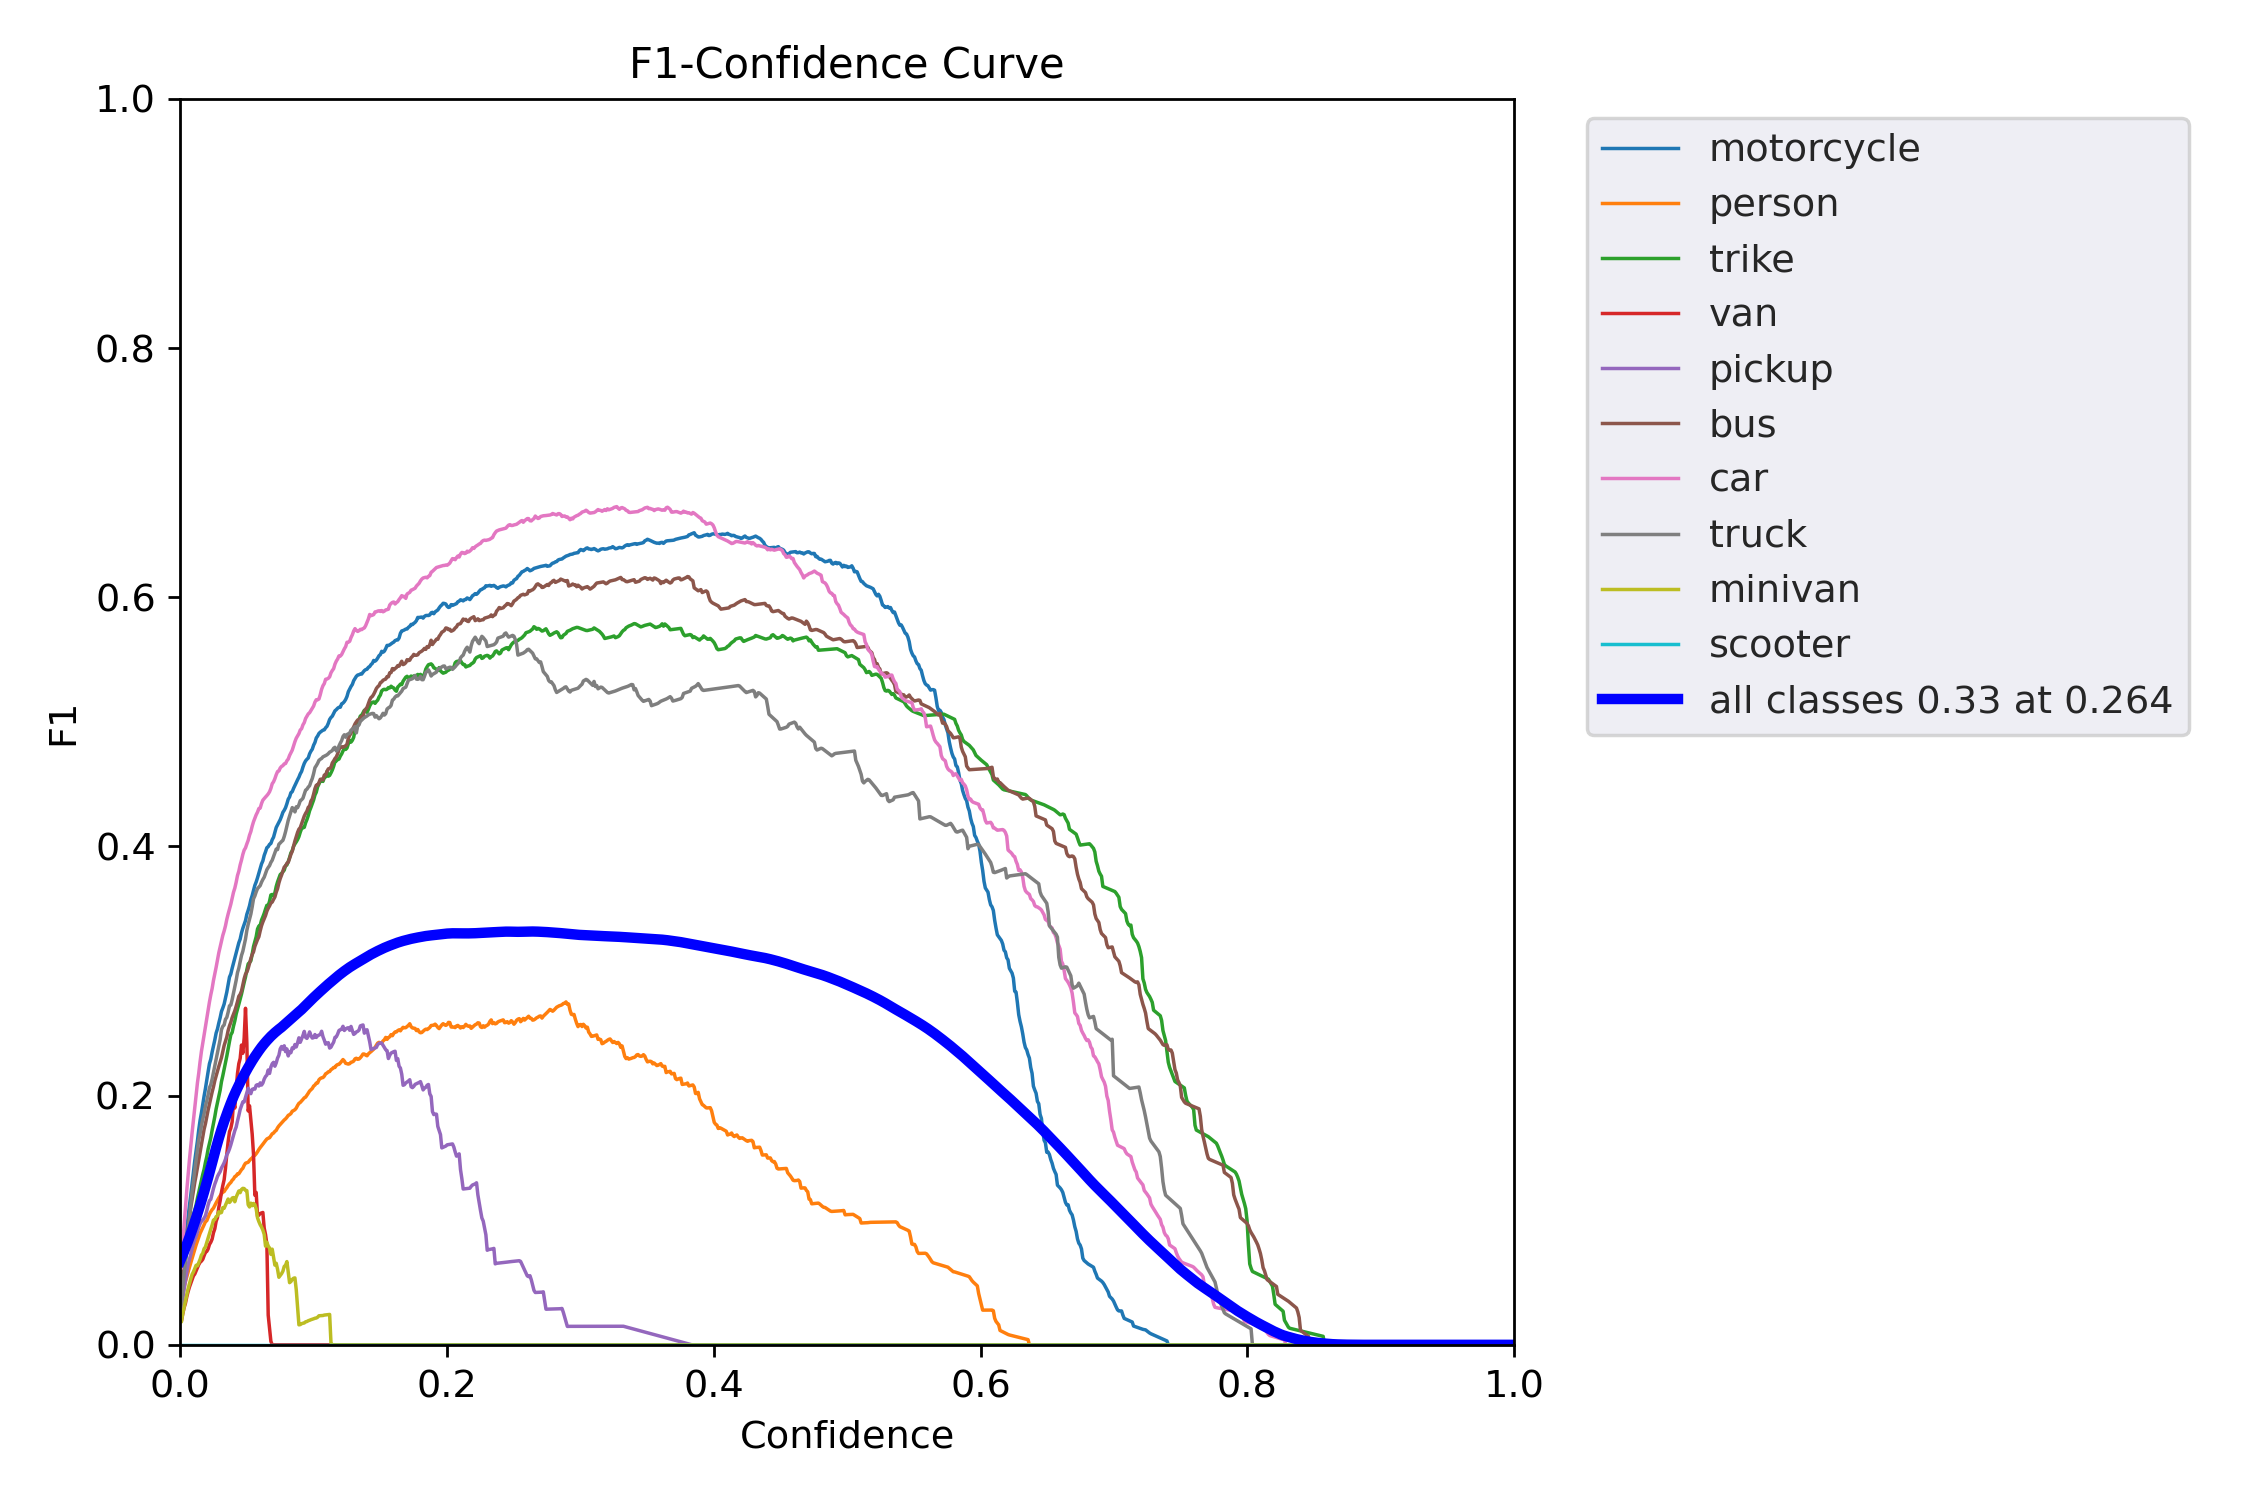
\includegraphics[width=.65\columnwidth]{Figures/dataset_c/F1_curve.png}
			\caption{Dataset C: F1 Confidence Curve of YOLOv5 model}
			\label{fig:ntDatasetYolov5MediumWeightF1Curve}
		\end{figure}

	\clearpage
	\section{Train vs. Prediction Batches}
		\subsection*{Daylight Models}
			Figures (\ref{fig:ukTrainBatchTwo},~\ref{fig:ukValBatchTwo},~\ref{fig:mtpTrainBatchTwo},~\ref{fig:mtpValBatchTwo}) show the training process of the third batch of the training and validation process. The training process of Dataset A, fig~\ref{fig:ukTrainBatchTwo}, classifies ten types of objects and applies a bounding box around the objects, labelling each bounding box with a classification number with an offset of minus one. Whereas the training process of Dataset B, fig~\ref{fig:mtpTrainBatchTwo}, classifies three objects with the same properties as the previous training process.

			For the validation process, the model tries to predict a selection of images and tries to detect objects within the image. This validation process helps us understand where the training process may be going wrong and helps us improve the training process. The validation figures (\ref{fig:ukValBatchTwo},~\ref{fig:mtpValBatchTwo}) have a new element on the bounding box, which indicates the confidence of the prediction. This information is next to the classification label, which is no longer a classification number. 
			\begin{figure}[ht]
				\floatsetup{valign=t, heightadjust=object}
				\begin{floatrow}
					\ffigbox[0.60\linewidth]
					{
						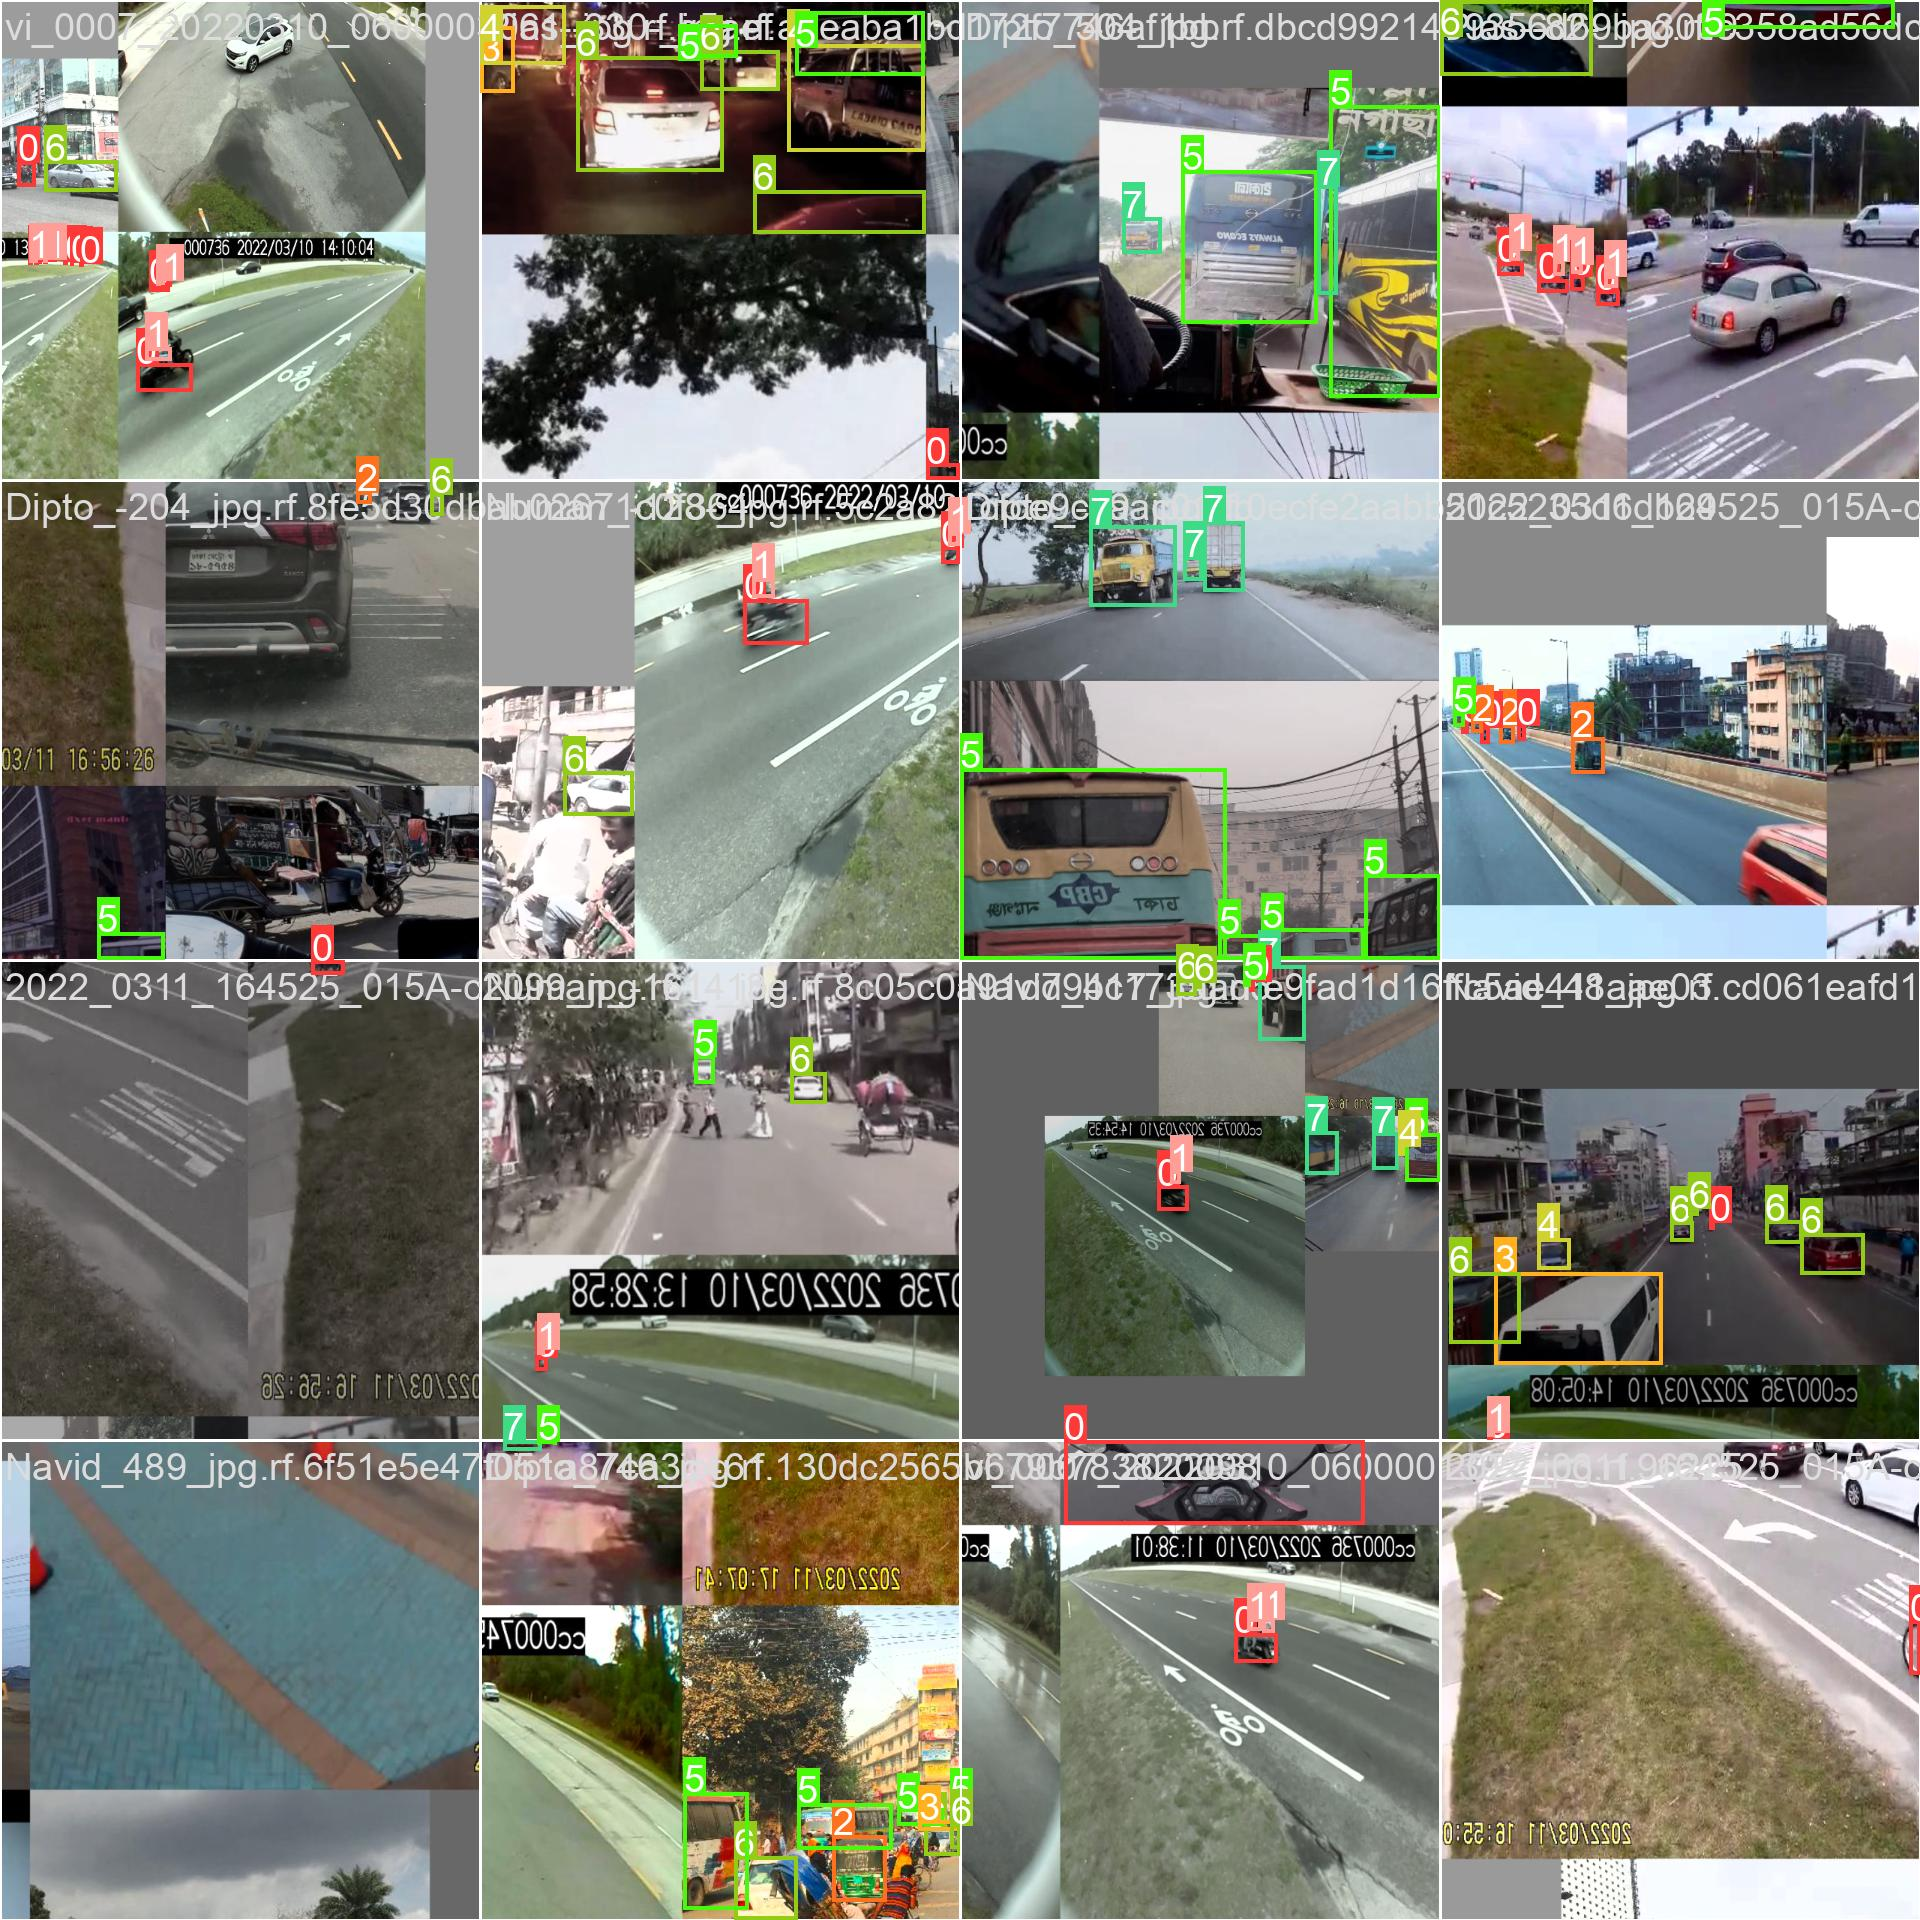
\includegraphics[width=1\linewidth]{Figures/dataset_a/train_batch2.jpg}
					}
					{
						\caption{Dataset A: Train Batch Two}
						\label{fig:ukTrainBatchTwo}
					}
				
					\ffigbox[0.60\linewidth]
					{
						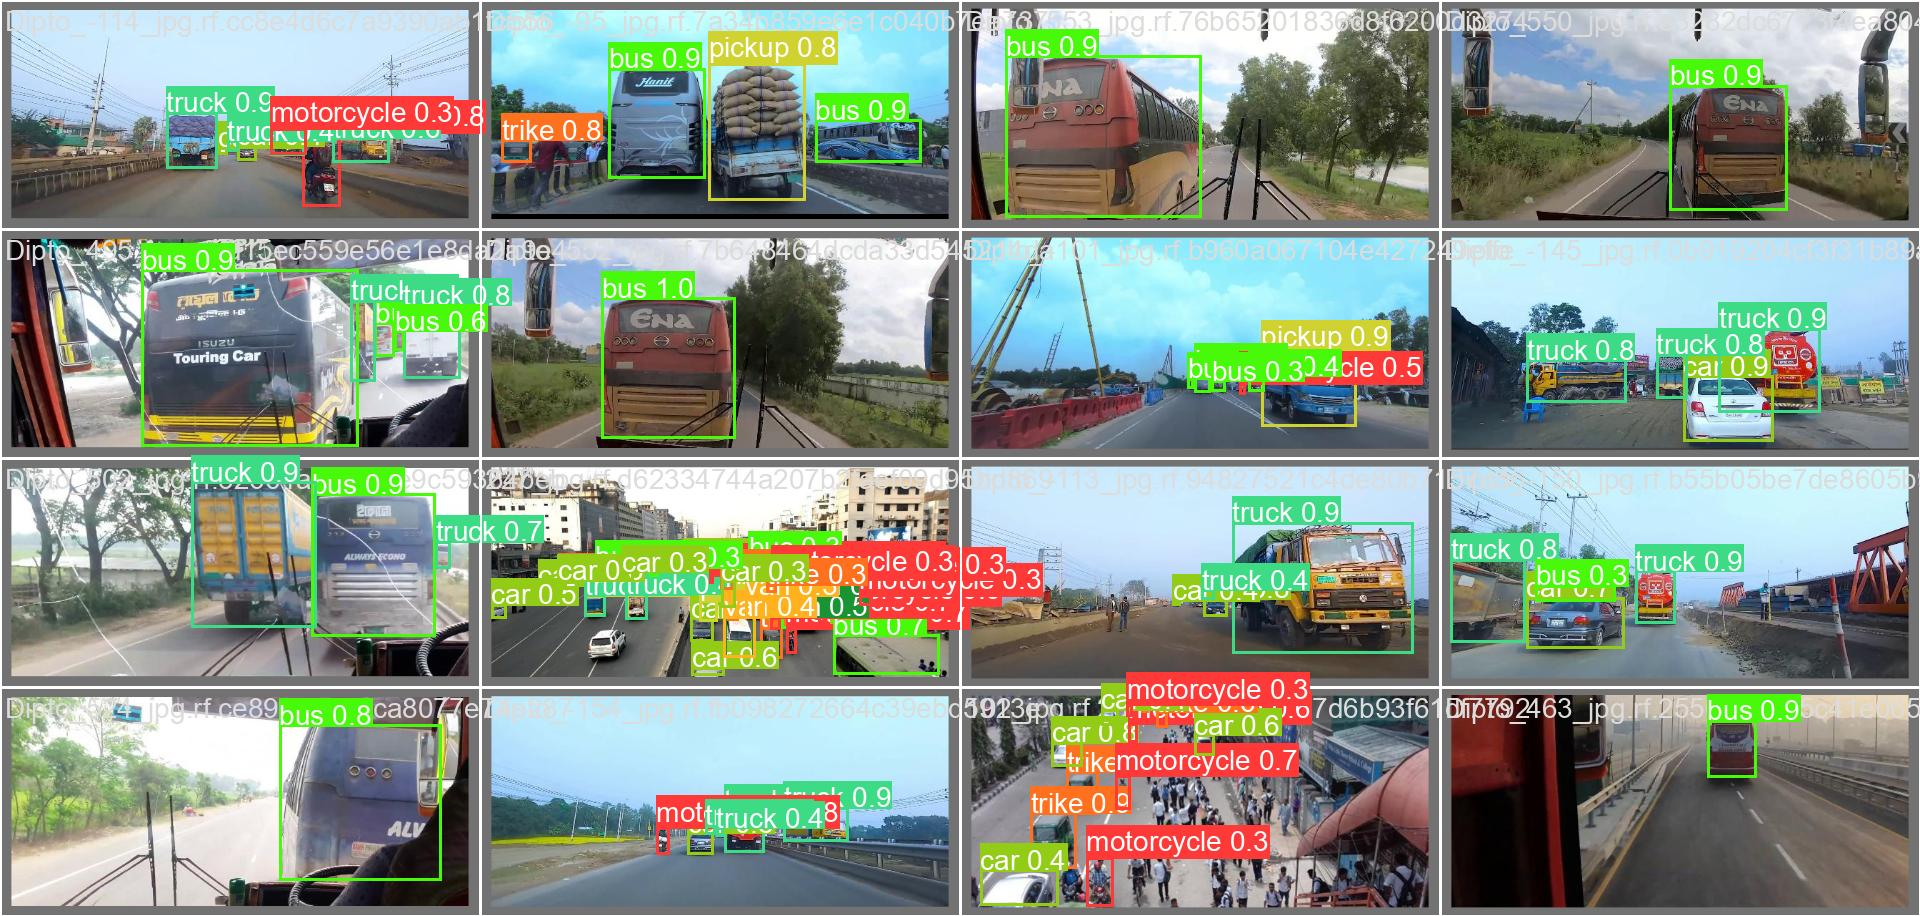
\includegraphics[width=1\linewidth]{Figures/dataset_a/val_batch2_pred.jpg}
					}
					{
						\caption{Dataset A: Validation Batch Two}
						\label{fig:ukValBatchTwo}
					}
				\end{floatrow}
			\end{figure}

			\begin{figure}[hb]
				\floatsetup{valign=t, heightadjust=object}
				\begin{floatrow}
					\ffigbox[0.60\linewidth]
					{
						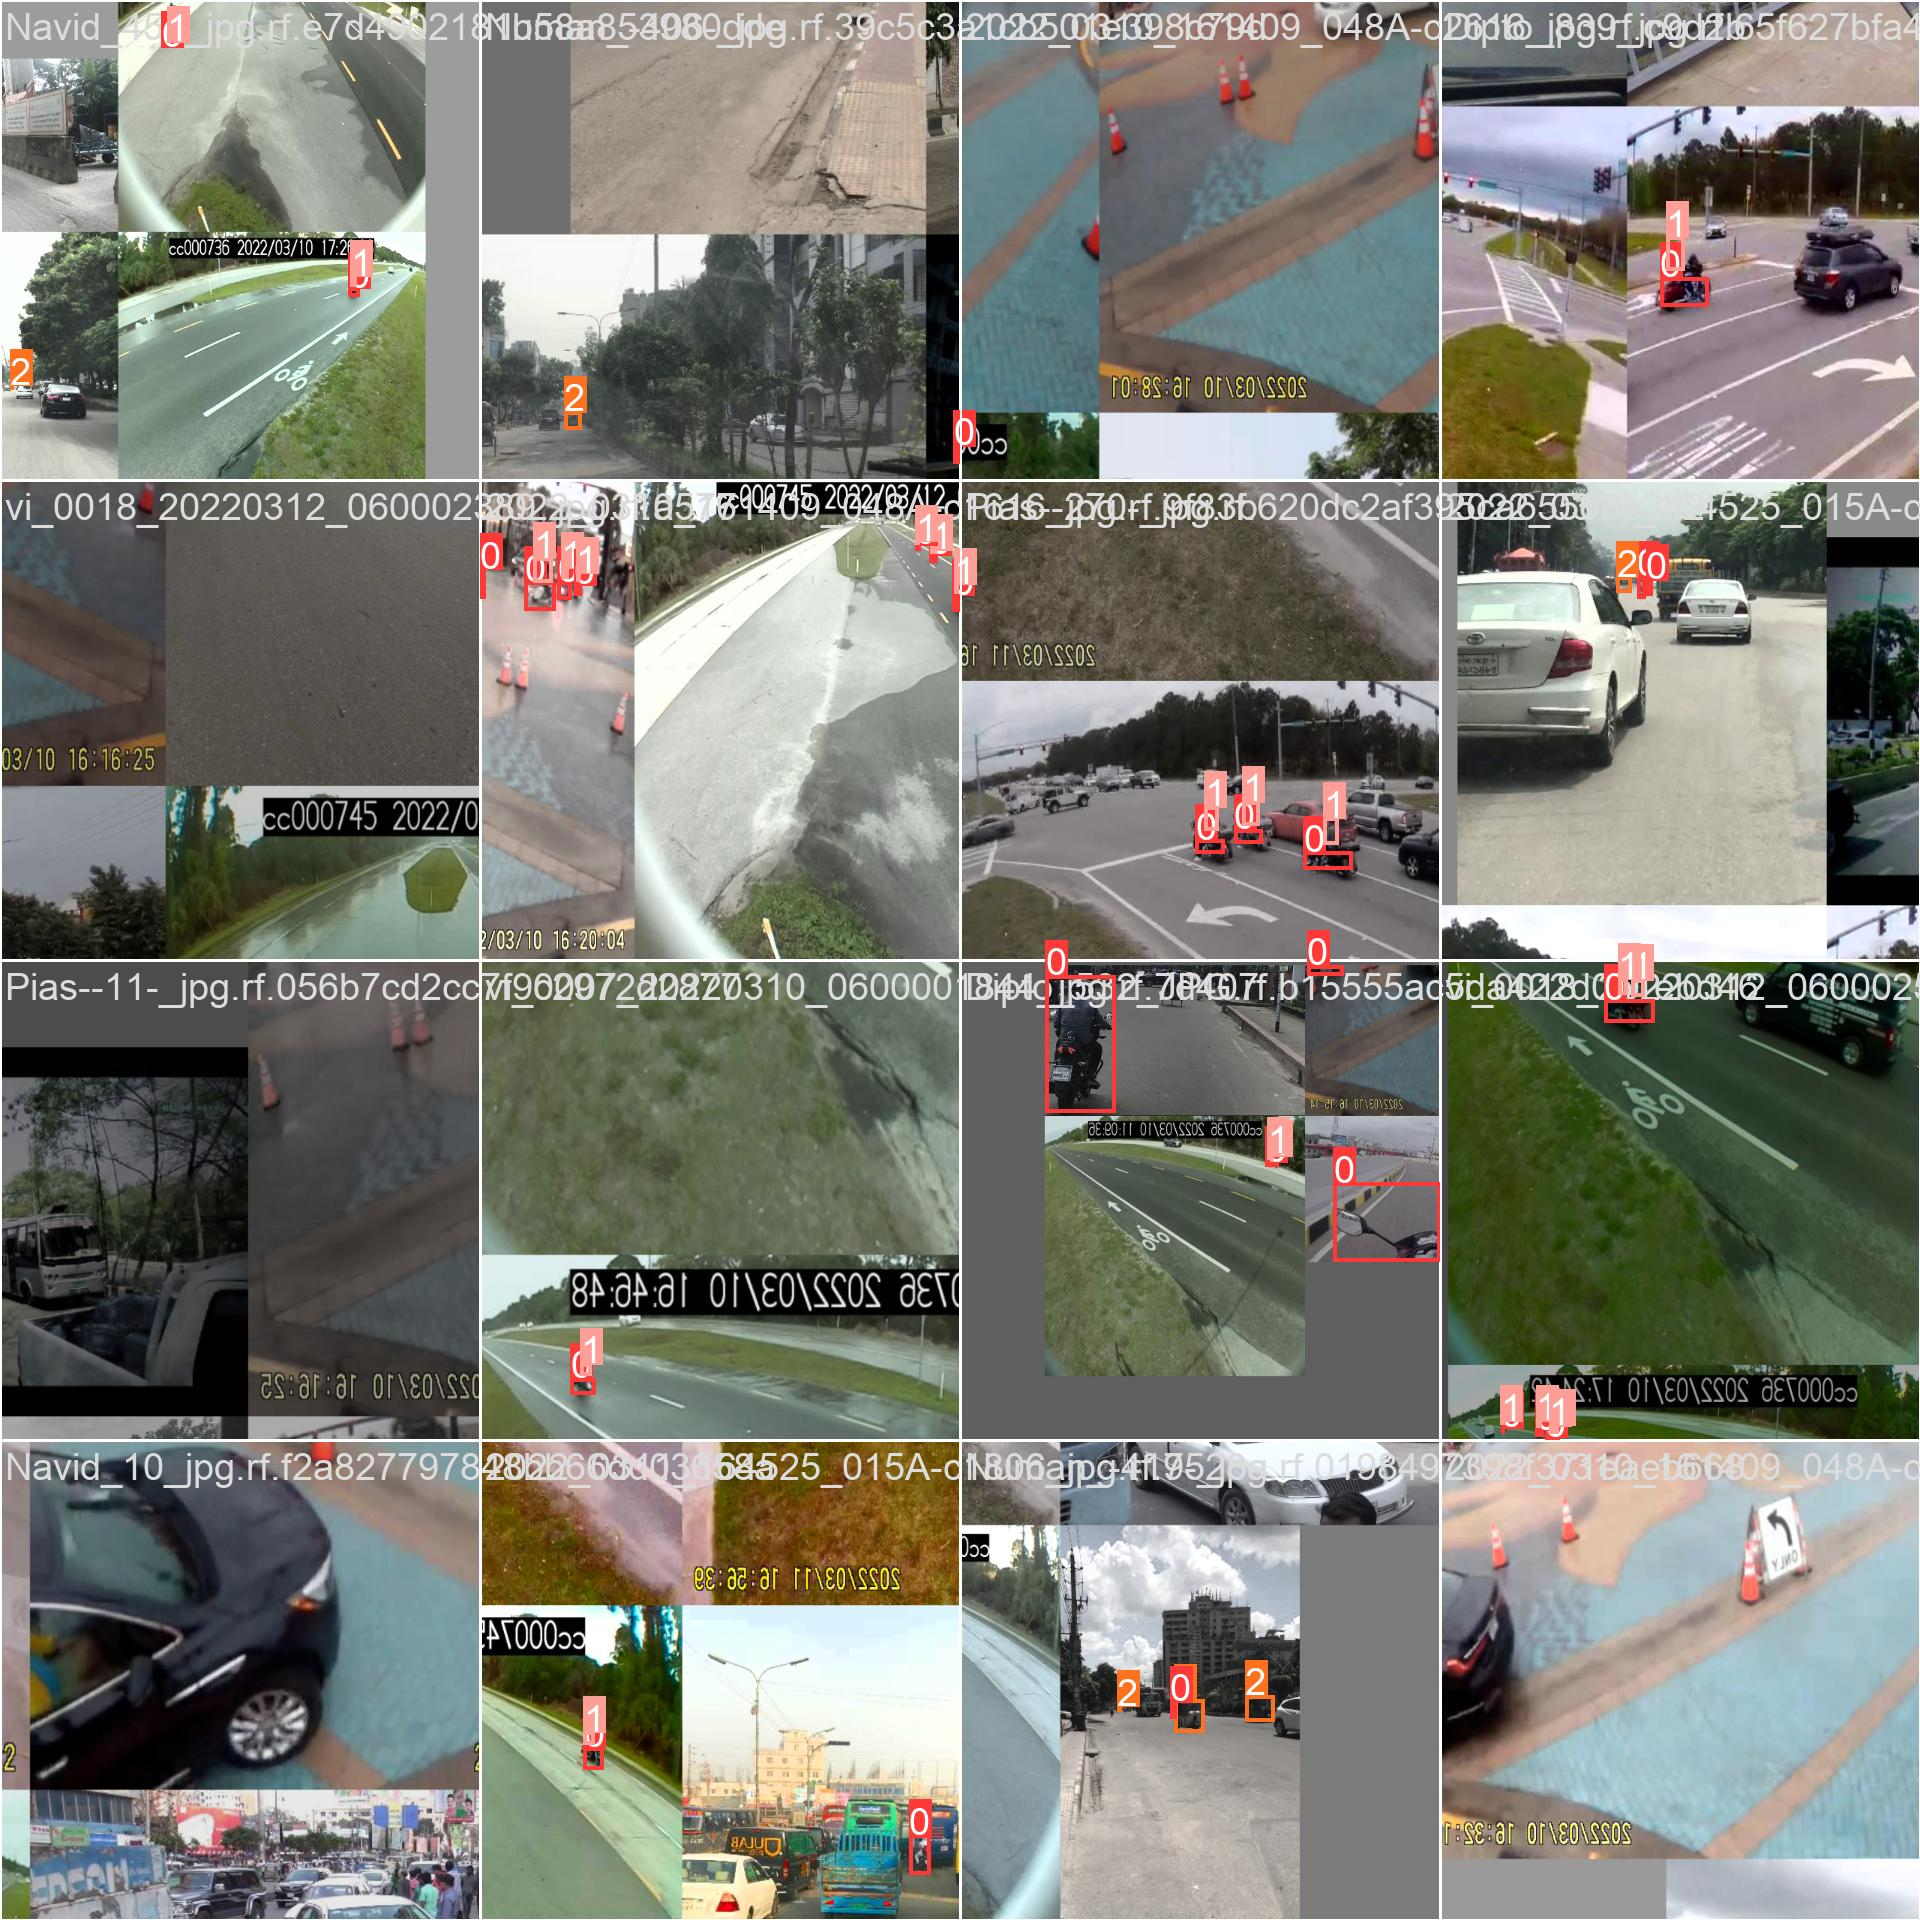
\includegraphics[width=1\linewidth]{Figures/dataset_b/train_batch2.jpg}
					}
					{
						\caption{Dataset B: Train Batch Two}
						\label{fig:mtpTrainBatchTwo}
					}
				
					\ffigbox[0.60\linewidth]
					{
						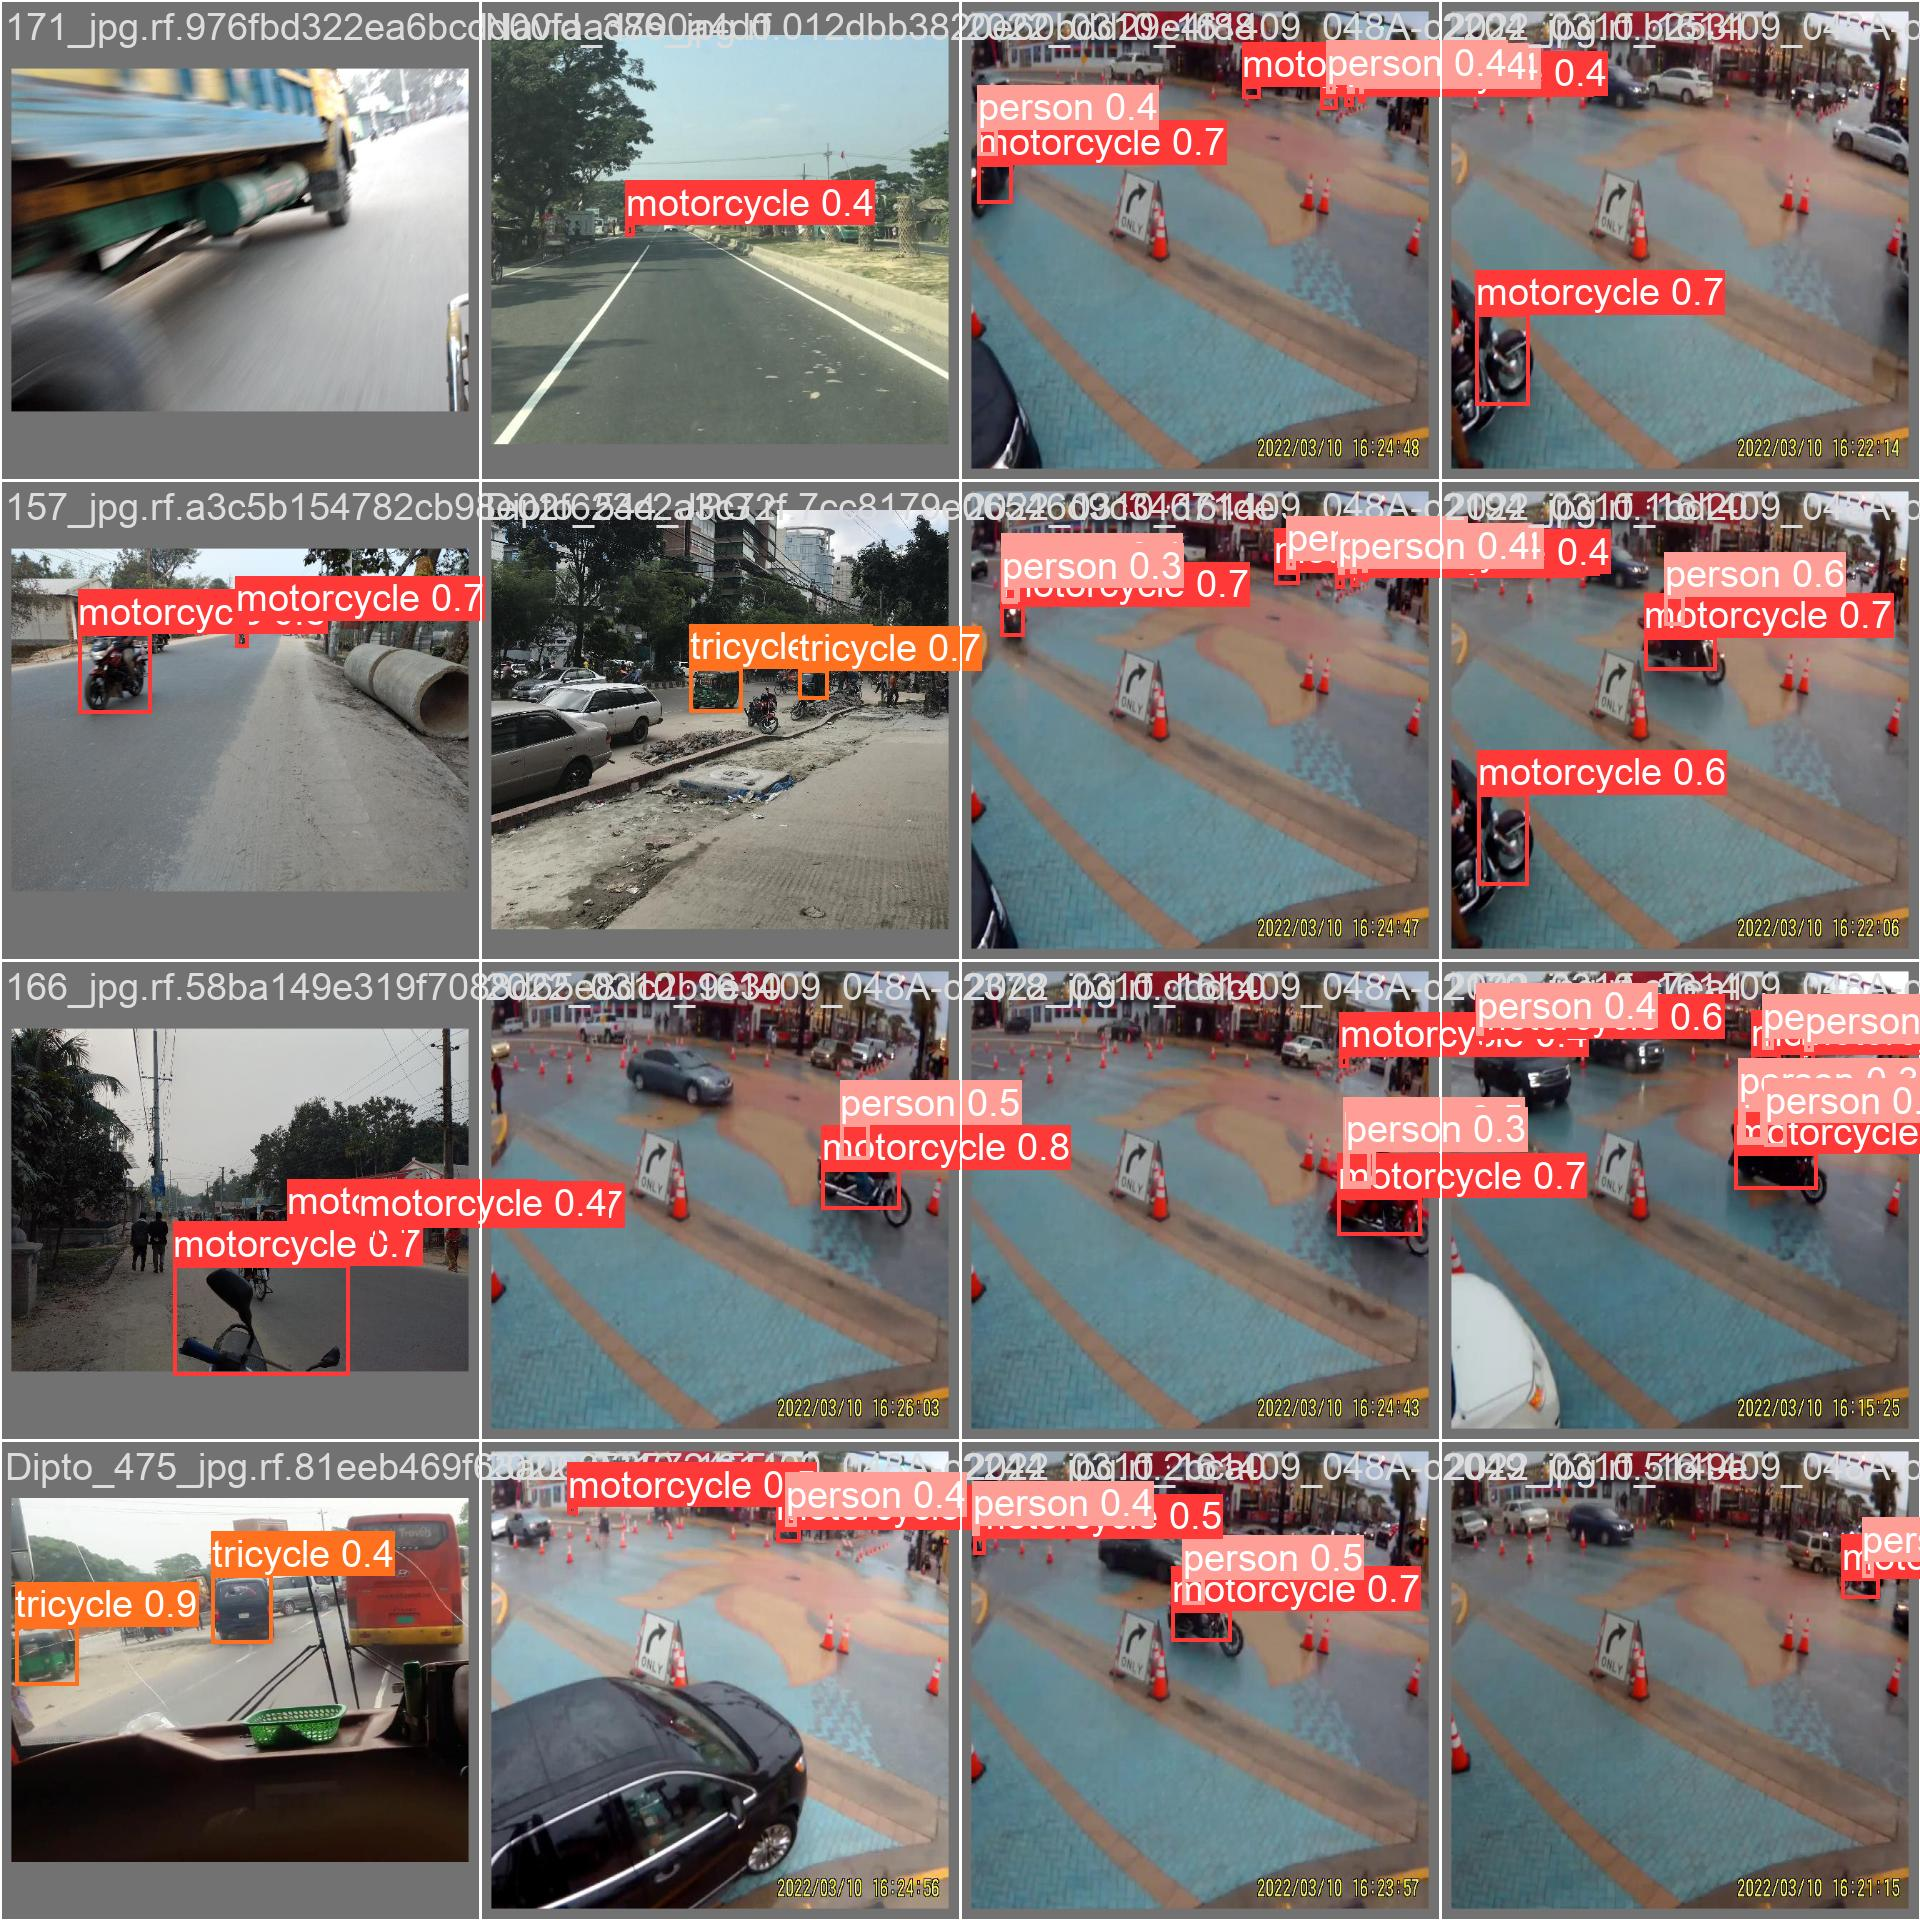
\includegraphics[width=1\linewidth]{Figures/dataset_b/val_batch2_pred.jpg}
					}
					{
						\caption{Dataset B: Validation Batch Two}
						\label{fig:mtpValBatchTwo}
					}
				\end{floatrow}
			\end{figure}
		
		\subsection*{Night-Time Models}
			Figures (\ref{fig:ntTrainBatchTwo},~\ref{fig:ntValBatchTwo}) illustrate the training and validation process of the night-time model, showing some key areas of how the dataset is modified. The illustration also shows the quality of the night-time simulation that the Python script achieved. From an observation, the images are harder to see motorcycles. However, it does not simulate the real night-time situation, on pitch-black roads. It is impressive to know that the model picks up motorcycles in this setup and should be the following best ideal environment for testing the model with actual footage.
			\begin{figure}[hb]
				\floatsetup{valign=t, heightadjust=object}
				\begin{floatrow}
					\ffigbox[0.60\linewidth]
					{
						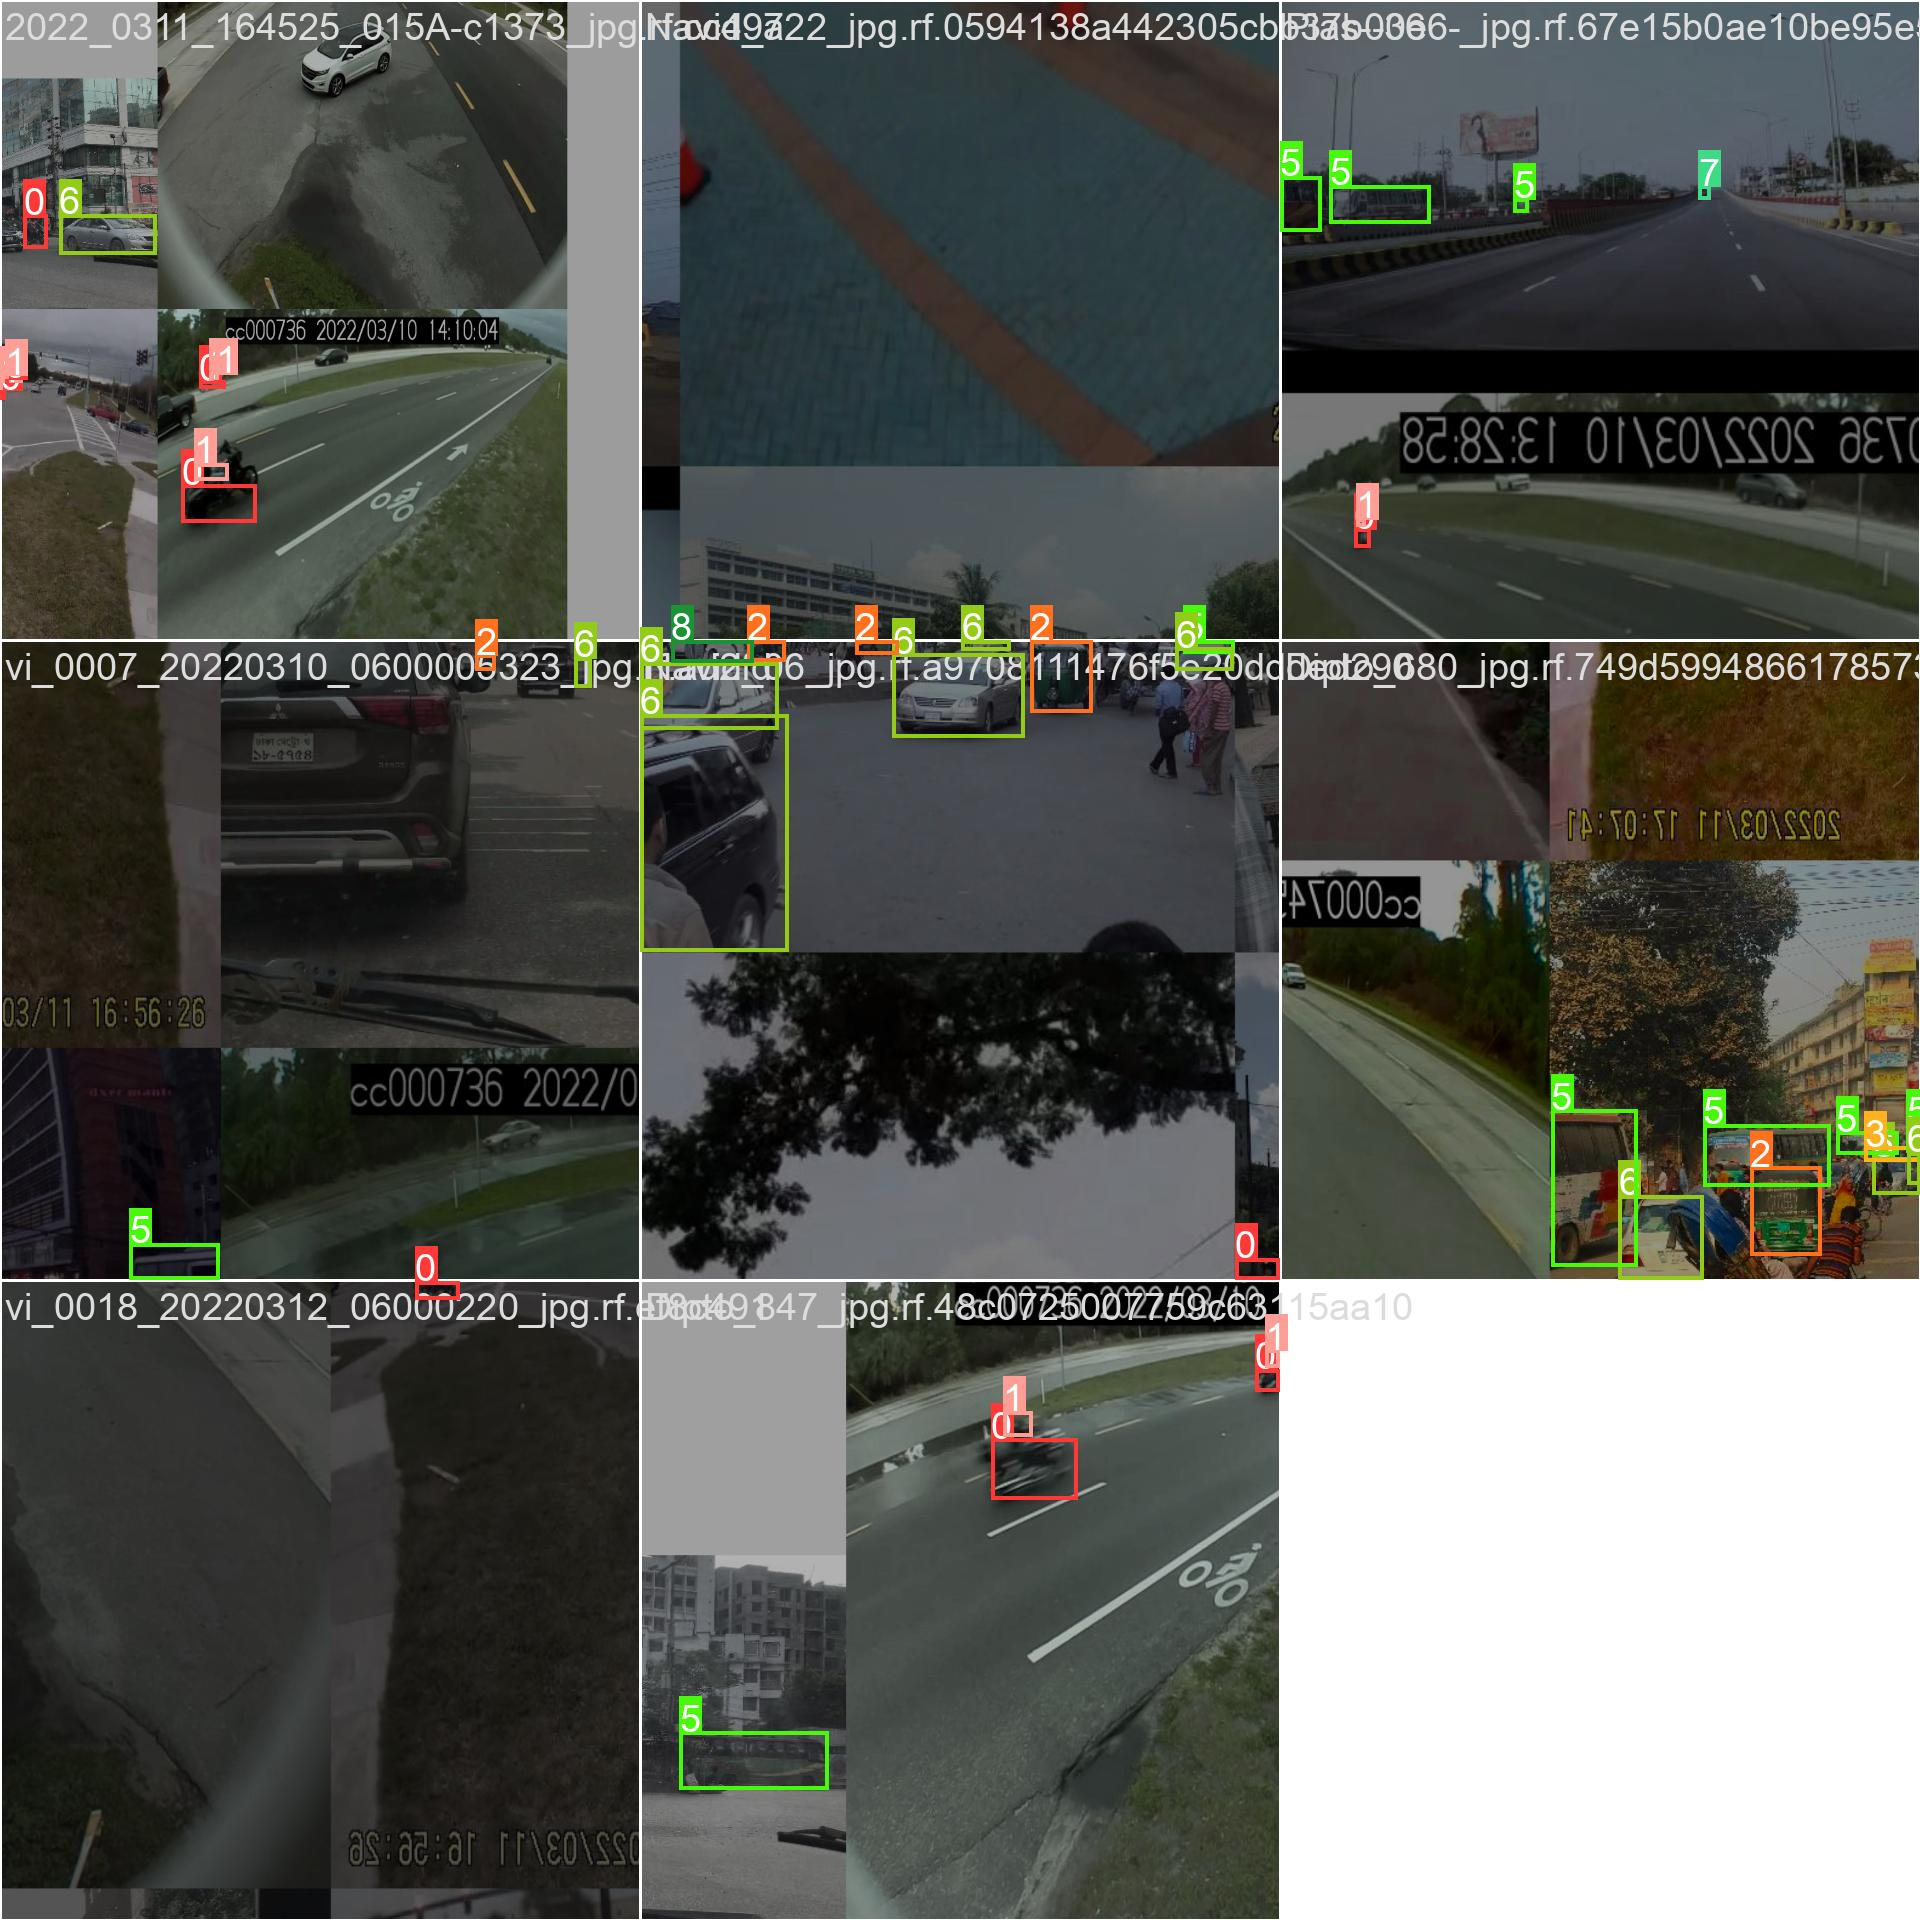
\includegraphics[width=1\linewidth]{Figures/dataset_c/train_batch2.jpg}
					}
					{
						\caption{Dataset C: Train Batch Two}
						\label{fig:ntTrainBatchTwo}
					}
				
					\ffigbox[0.60\linewidth]
					{
						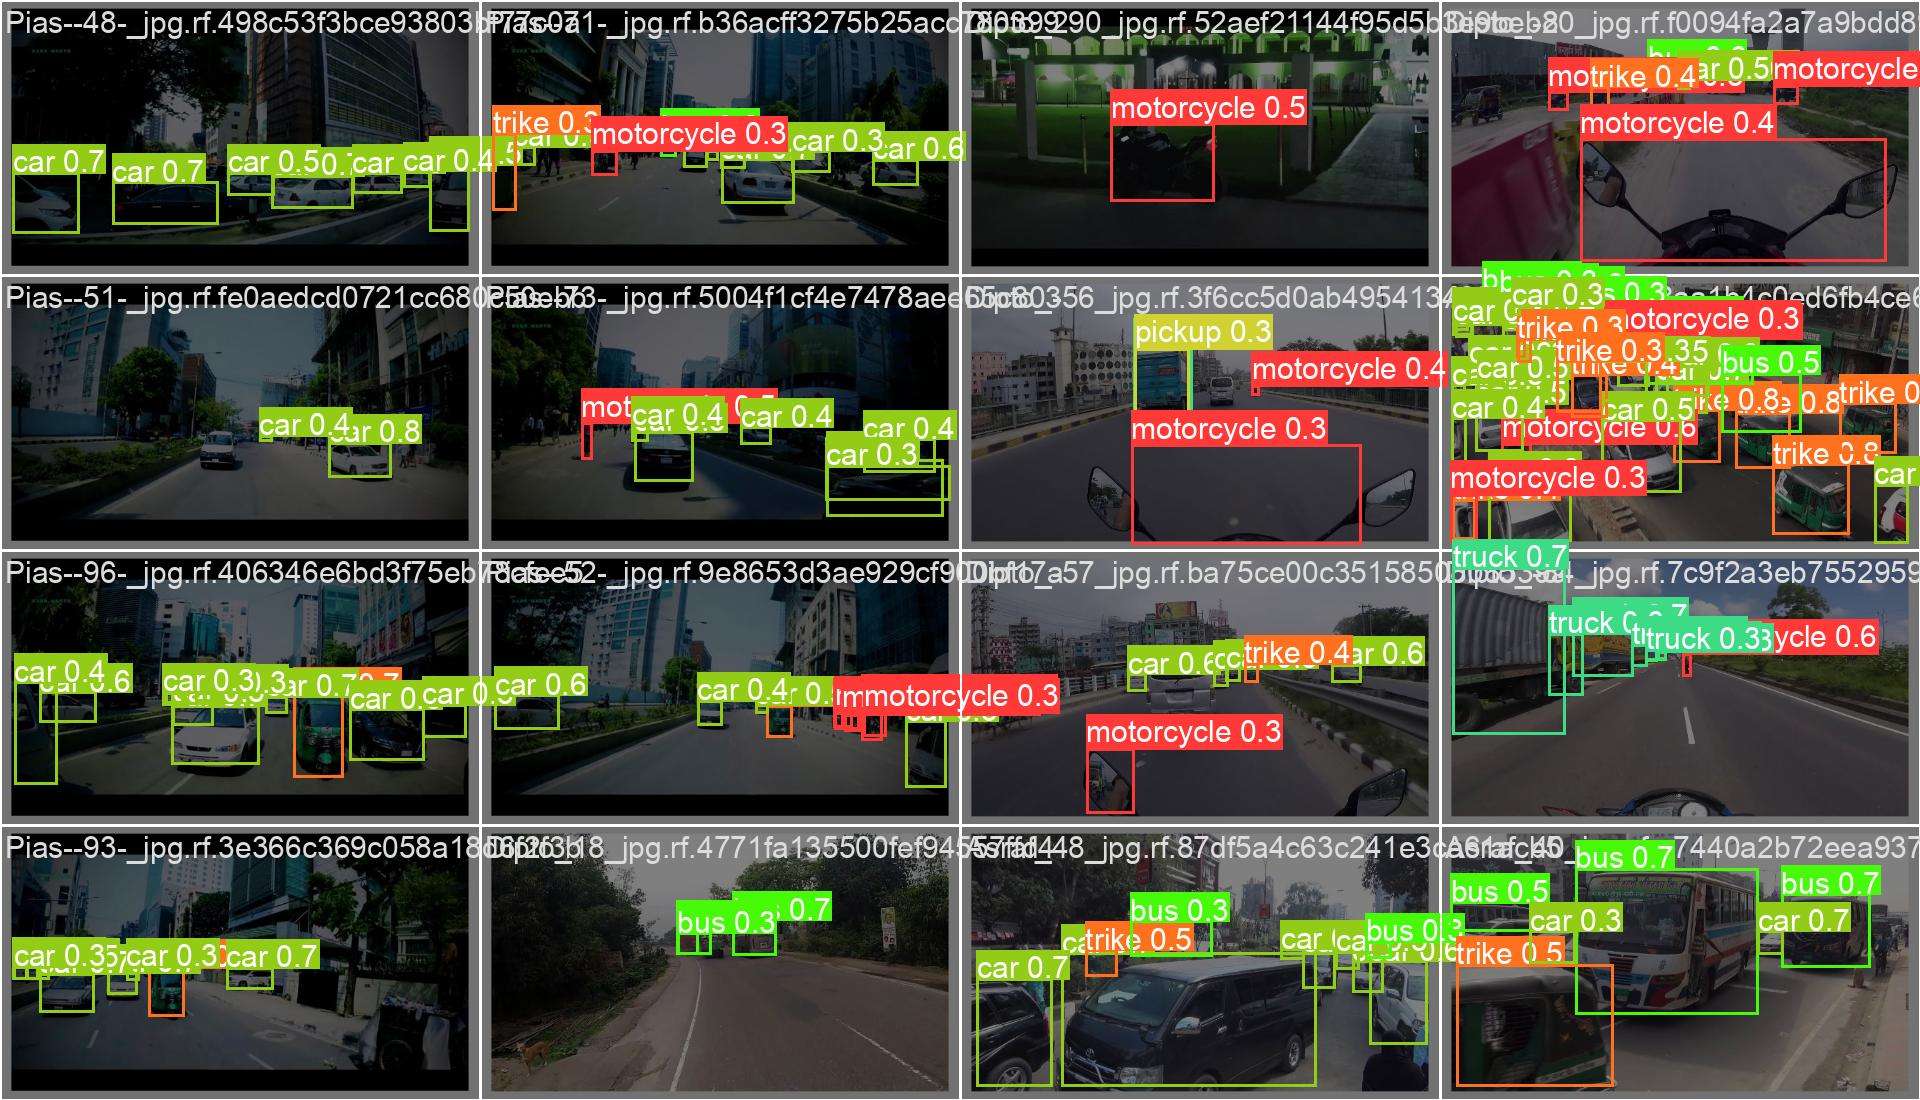
\includegraphics[width=1\linewidth]{Figures/dataset_c/val_batch2_pred.jpg}
					}
					{
						\caption{Dataset C: Validation Batch Two}
						\label{fig:ntValBatchTwo}
					}
				\end{floatrow}
			\end{figure}
		
	\clearpage
	\section{Labels}
		Figures (\ref{fig:ukDatasetYolov5LargeWeightLabels},~\ref{fig:mtpDatasetYolov5LargeWeightLabels},~\ref{fig:ntDatasetYolov5MediumWeightLabels}) showcases the four methods of identification of labels. The top-left chart depicts the instances when a class was plotted. The top-right displays the sizes of the labels in correspondence with the colour key from the top-left. The bottom-left scatter graphs show the positioning of where the labels were plotted, and the bottom-right displays the size of the labels. The main focus areas would be the labelling, box size, and volume of the sizes to indicate if the labels were plotted accurately. Each of the datasets did a decent job of choosing the box dimensions. However, some dimensions were not vertical and were horizontal, which is evident that a problem the model was doing was detecting the handlebars on the camera as a motorcycle, which indicates why the labels were horizontal. This observation explains why its labels appear horizontal and do not necessarily mislabel a car. Another reason for this is that motorcycles may be parked or detected sideways, allowing a rendering of a horizontal bounding box.
		\begin{figure}[ht]
			\floatsetup{valign=t, heightadjust=object}
			\begin{floatrow}
				\ffigbox[0.63\linewidth]
				{
					\includegraphics[width=1\linewidth]{Figures/dataset_a/labels.jpg}
				}
				{
					\caption{Dataset A: Performance and Recall Curve of YOLOv5 model}
					\label{fig:ukDatasetYolov5LargeWeightLabels}
				}
			
				\ffigbox[0.63\linewidth]
				{
					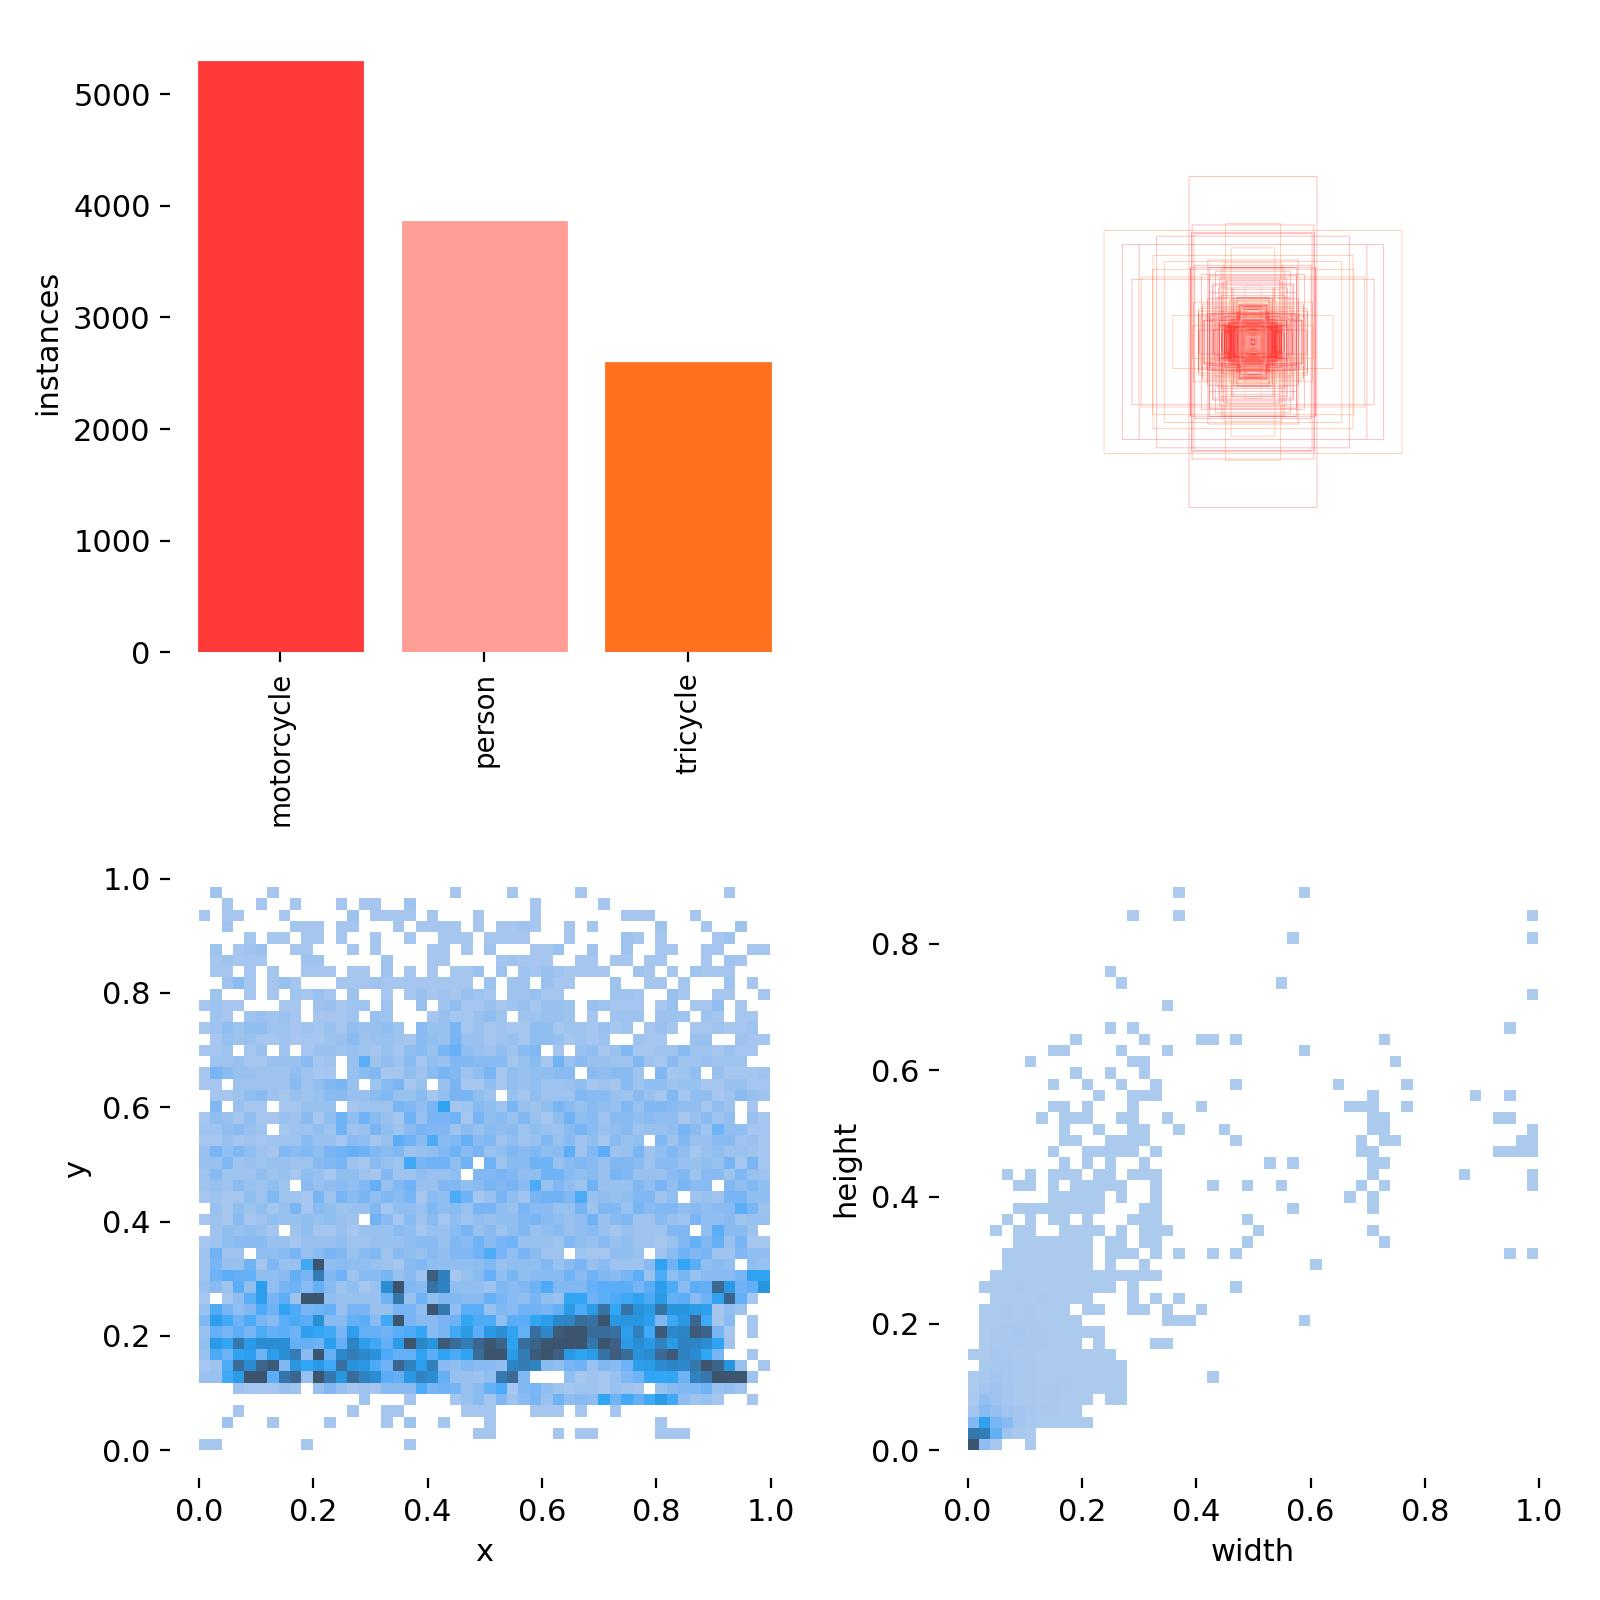
\includegraphics[width=1\linewidth]{Figures/dataset_b/labels.jpg}
				}
				{
					\caption{Dataset B: Performance and Recall of YOLOv5 model}
					\label{fig:mtpDatasetYolov5LargeWeightLabels}
				}
			\end{floatrow}
		\end{figure}

		\begin{figure}[hb]
			\centering
			\includegraphics[width=.43\columnwidth]{Figures/dataset_c/labels.jpg}
			\caption{Dataset C: Performance and Recall of YOLOv5 model}
			\label{fig:ntDatasetYolov5MediumWeightLabels}
		\end{figure}

\chapter{Findings}
\label{chap:findings}
	\section{Wet and Poor Visibility}
		The following images of~\ref{fig:detectionOfMotorcycleW1},~\ref{fig:detectionOfMotorcycleW2} and~\ref{fig:detectionOfMotorcycleW3} show different wet condition scenarios. Due to previous research conducted, according to Tesla, ``Tesla announces in 2021 that the company would remove a sensor called Ultrasonic Sensors, replacing the sensor with `Tesla Vision' by 2022''.~\cite{noauthor_tesla_nodate} This only means according to ``Self-Driving Cars and The Law: Putting autonomous vehicles on the road isn't just a matter of fine-tuning technology'' by Nathan A. Greenblatt, that AVs used `...thanks to lidar, radar, and ultrasonic sensors, they can see through fog and in the dark.', meaning that Tesla AVs for example, only use a visual aid to see. However, this raises concerns about the reliability of AVs solely using visual input. In situations where the camera's view is obscured by wet patches or heavy fog, a human driver could outperform the technology.

		Figure~\ref{fig:detectionOfMotorcycleW1} of a motorcycle in wet weather conditions, the architecture trained weight has successfully found the motorcycle with 75\% positiveness that it is a motorcycle.

		Figure~\ref{fig:detectionOfMotorcycleW2} of a motorcycle in wet weather conditions, the architecture failed to find the motorcycle. This scenario happened when the water content blurred the camera, which could simulate current problems with vision technology within AVs.

		Figure~\ref{fig:detectionOfMotorcycleW3} of a motorcycle in wet weather conditions, the architecture failed to find the motorcycle. The visibility is moderate; human eyesight can easily see more than eight to ten meters ahead. Another observation of this footage was that the vehicles are visible, although the architecture failed to recognise the motorcycle.
		\begin{figure}[hb]
			\floatsetup{valign=t, heightadjust=object}
			\begin{floatrow}
				\ffigbox[0.70\linewidth]
				{
					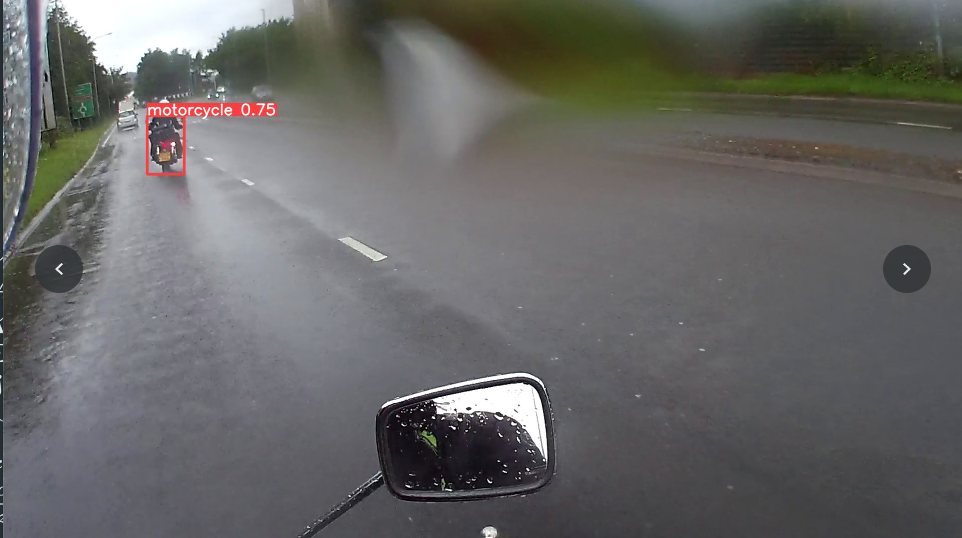
\includegraphics[width=1.1\linewidth]{Figures/scenarios/wet_correct.png}
				}
				{
					\caption{Good Detection of Motorcycle - Wet and Multi Lane}
					\label{fig:detectionOfMotorcycleW1}
				}
			
				\ffigbox[0.70\linewidth]
				{
					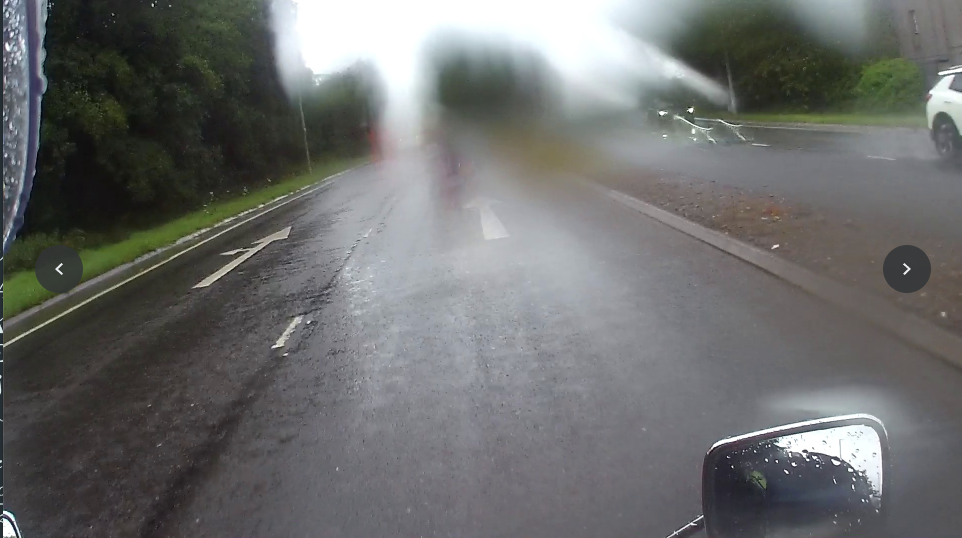
\includegraphics[width=1.1\linewidth]{Figures/scenarios/wet_incorrect.png}
				}
				{
					\caption{Classification Error - Camera Blinded}
					\label{fig:detectionOfMotorcycleW2}
				}
			
				\ffigbox[0.70\linewidth]
				{
					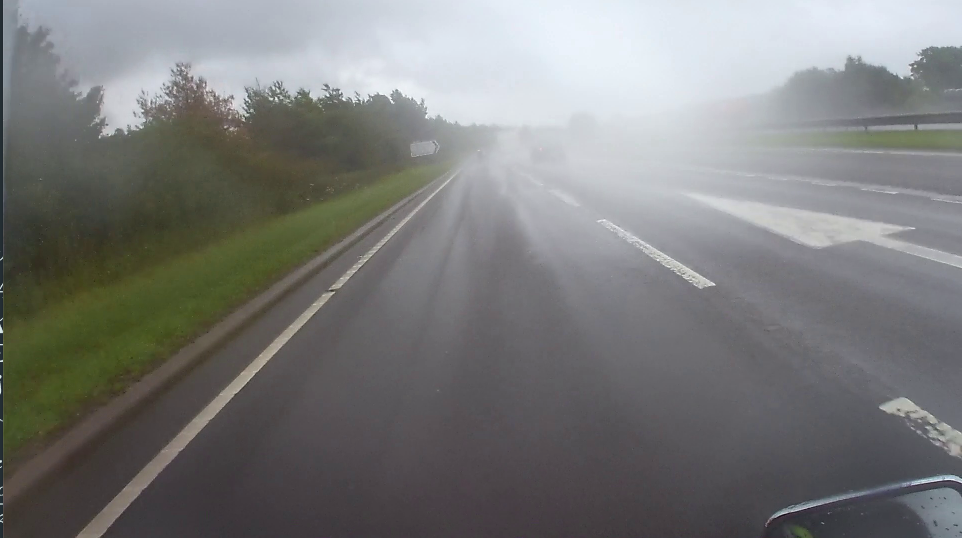
\includegraphics[width=1.1\linewidth]{Figures/scenarios/wet_danger.png}
				}
				{
					\caption{Classification Error - Water Spray from Other Vehicles}
					\label{fig:detectionOfMotorcycleW3}
				}
			\end{floatrow}
		\end{figure}

	\section{Blindspot and Late Classifications}
		Figure~\ref{fig:detectionOfOneMotorcycle} of detecting one motorcycle may not seem dangerous. However, if an AV misclassifies or does not detect the motorcycle after the first motorcycle, the AV may not be able to foresee any sudden traffic actions, causing fatal collisions.

		Figures~\ref{fig:lateClassificationP1},~\ref{fig:lateClassificationP2} demonstrates the dangers of motorcycle misclassification near a junction. If the AV were to turn right, coming out of the junction, then due to the AV not anticipating the motorcyclist, then the AV may pull out on the motorcycle, causing a fatality. The Object Classification did, however, detect the motorcycle when it was closer to the motorcycle.
		\begin{figure}[ht]
			\floatsetup{valign=t, heightadjust=object}
			\begin{floatrow}
				\ffigbox[0.70\linewidth]
				{
					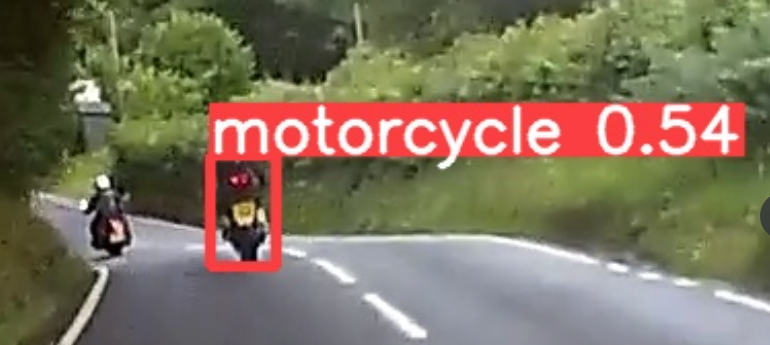
\includegraphics[width=1\linewidth]{Figures/scenarios/fail.png}
				}
				{
					\caption{Detection of One Motorcycle}
					\label{fig:detectionOfOneMotorcycle}
				}
			
				\ffigbox[0.70\linewidth]
				{
					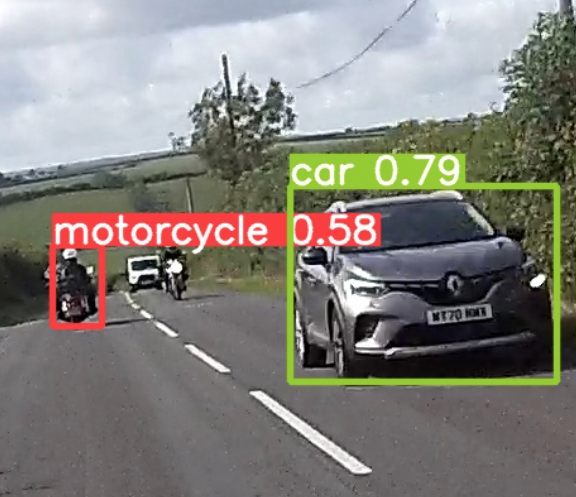
\includegraphics[width=0.9\linewidth]{Figures/scenarios/left_turn.png}
				}
				{
					\caption{Late Classification - Part 1}
					\label{fig:lateClassificationP1}
				}
			
				\ffigbox[0.70\linewidth]
				{
					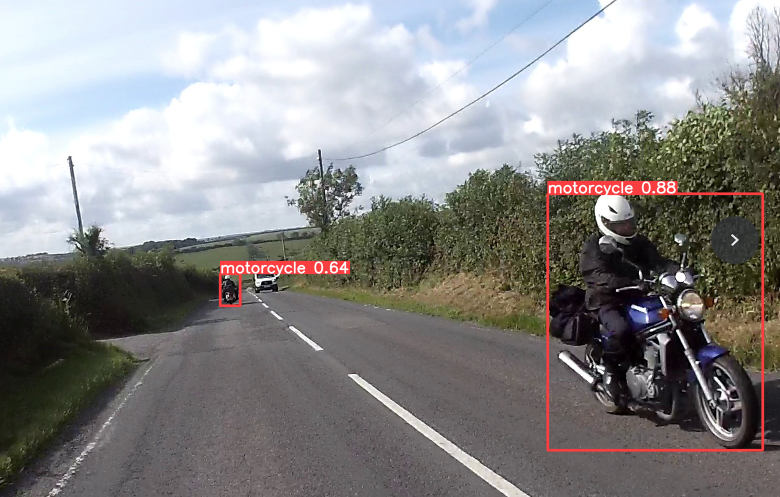
\includegraphics[width=0.9\linewidth]{Figures/scenarios/motorcycle.png}
				}
				{
					\caption{Late Classification - Part 2}
					\label{fig:lateClassificationP2}
				}
			\end{floatrow}
		\end{figure}


		Figure~\ref{fig:overtakingSequence} shows a 75\% accuracy of correctly identifying two motorcycles after two overtakes. However, the last sequence shows an overtaking procedure involving two tractors and two motorcycles. The classification process is concerning, considering the motorcycles were not detected. This concern arises from a few things, the AV could perform an overtaking manoeuvre and accelerate unsafely, or if an AV started approaching at the speed limit, the AV might not slow down, even though other traffic is overtaking behind the riders to get by tractors safely.
		\begin{figure}[hb]
			\centering
			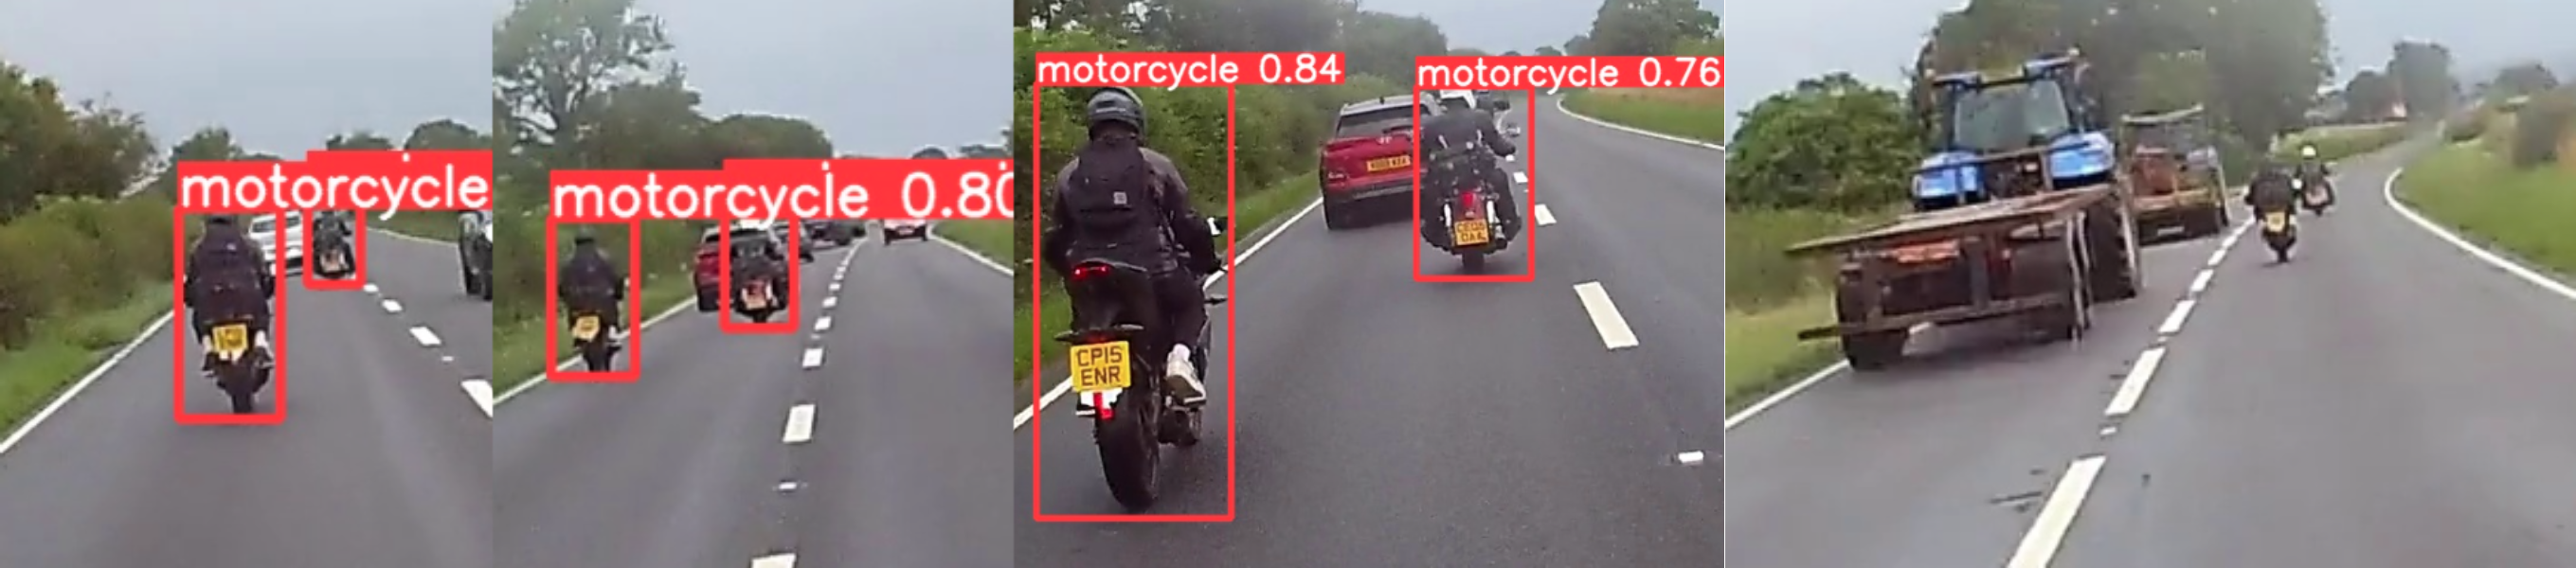
\includegraphics[width=\columnwidth]{Figures/scenarios/motorcycle_overtaking_sequence.png}
			\caption{Overtaking Sequence}
			\label{fig:overtakingSequence}
		\end{figure}

		\clearpage
		Figures (\ref{fig:dtSimulatedBlindspotP1},~\ref{fig:dtSimulatedBlindspotP2},~\ref{fig:dtSimulatedBlindspotP3}) simulates a blindspot to the left side of the camera to capture any motorcyclists. A pillion with a mounted camera was used as an idea that the helmet could lesson the area available, which could make simulated blindspots for the model to try to detect. The experiment idea appears to works well when simulating blindspots with the resources available.
		
		Each figure has a motorcyclist located on the left position. The motorcyclist is wearing black, with white reflectors safety gear. Even though human intelligence can easily see the motorcyclist, the object classification may not be as it blends in the camera footage. The sun is coming down, allowing the motorcyclist to blend in. As the motorcyclist and vehicle appear in fig~\ref{fig:dtSimulatedBlindspotP2}, the object classification still has not got enough information to detect the object until fig~\ref{fig:dtSimulatedBlindspotP3}, where the motorcyclist is fully seen. A problem located in this scenario is that the motorcyclist is breaking the whole way, but if a motorcyclist was in any blindspots of cameras, the AV may never know, and if the motorcyclist was indicating, then the motorcyclist stands no chance if an evasive manoeuvre had to happen.
		\begin{figure}[ht]
			\centering
			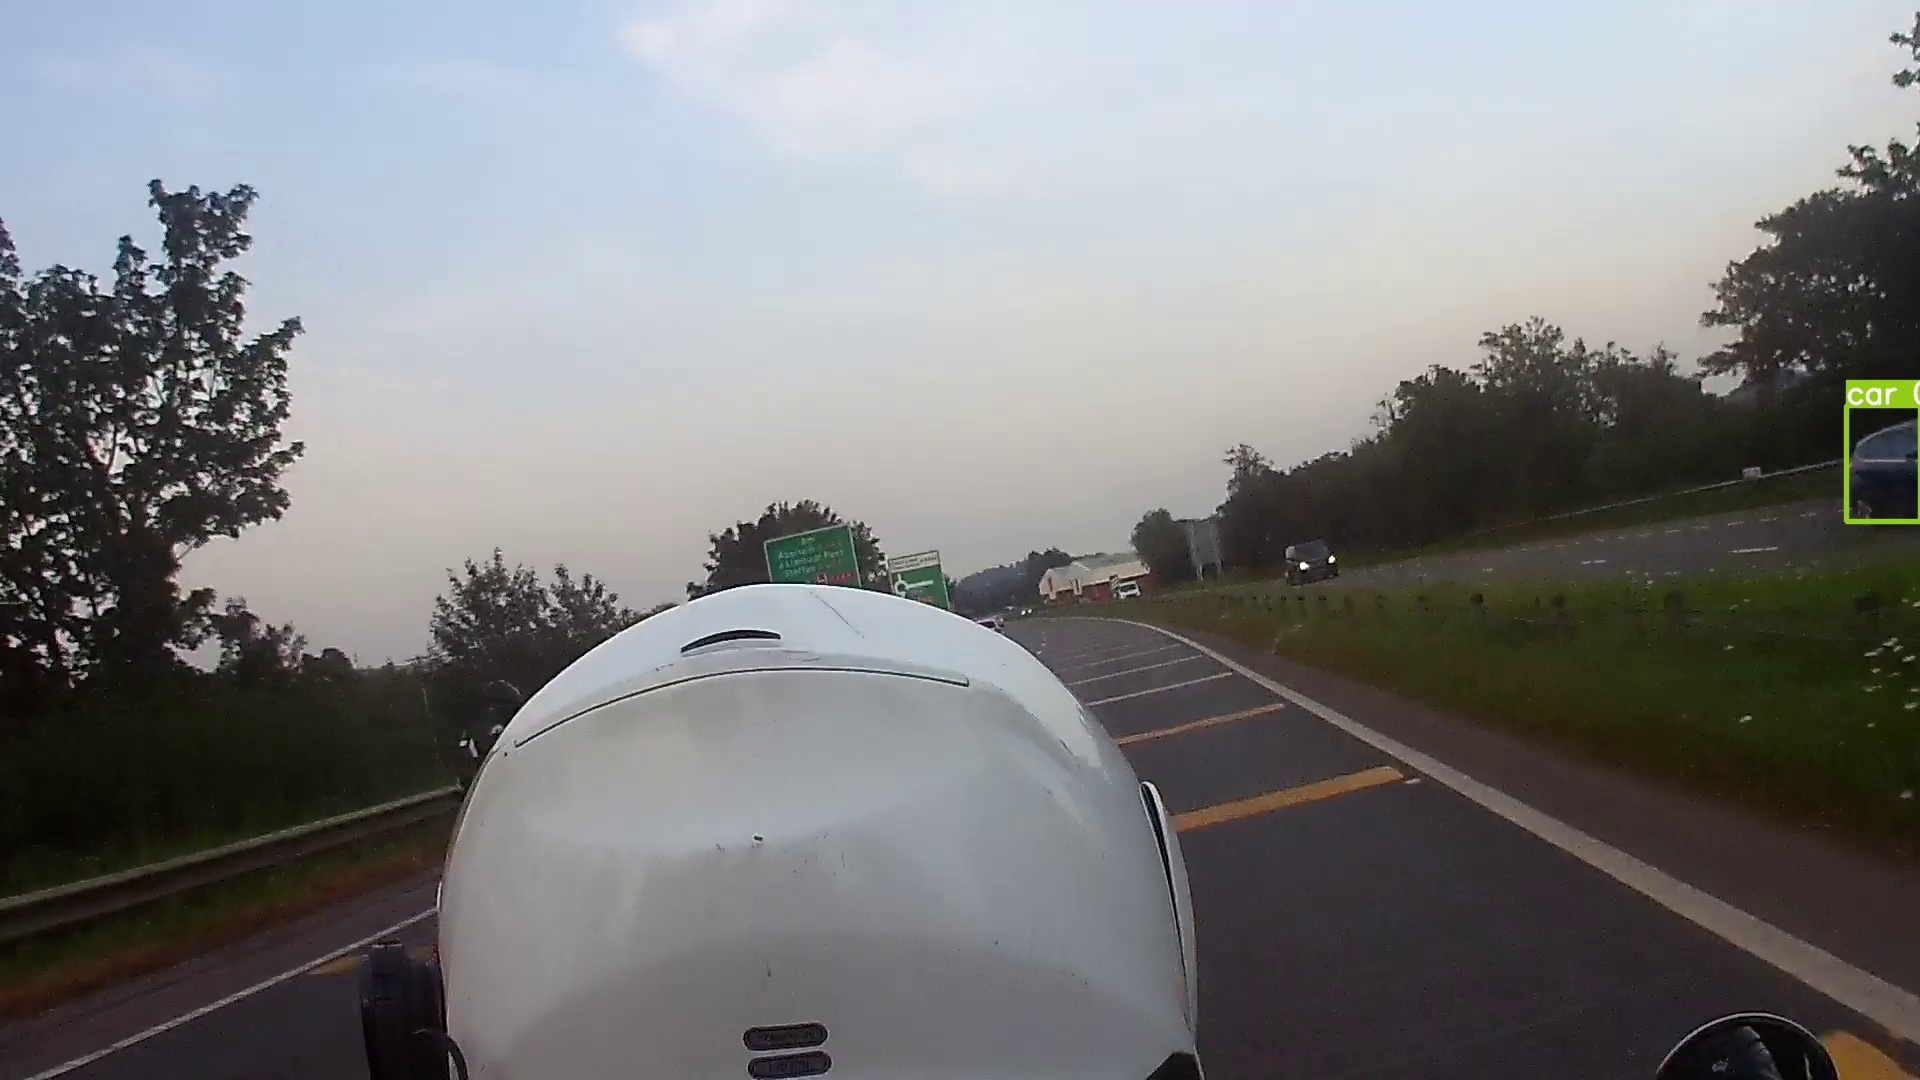
\includegraphics[width=.74\columnwidth]{Figures/scenarios/blindspot_day_t1/Misc_T4-334.jpg}
			\caption{Daytime Simulated Blindspot - Part 1}
			\label{fig:dtSimulatedBlindspotP1}
		\end{figure}

		\begin{figure}[hb]
			\floatsetup{valign=t, heightadjust=object}
			\begin{floatrow}
				\ffigbox[1\linewidth]
				{
					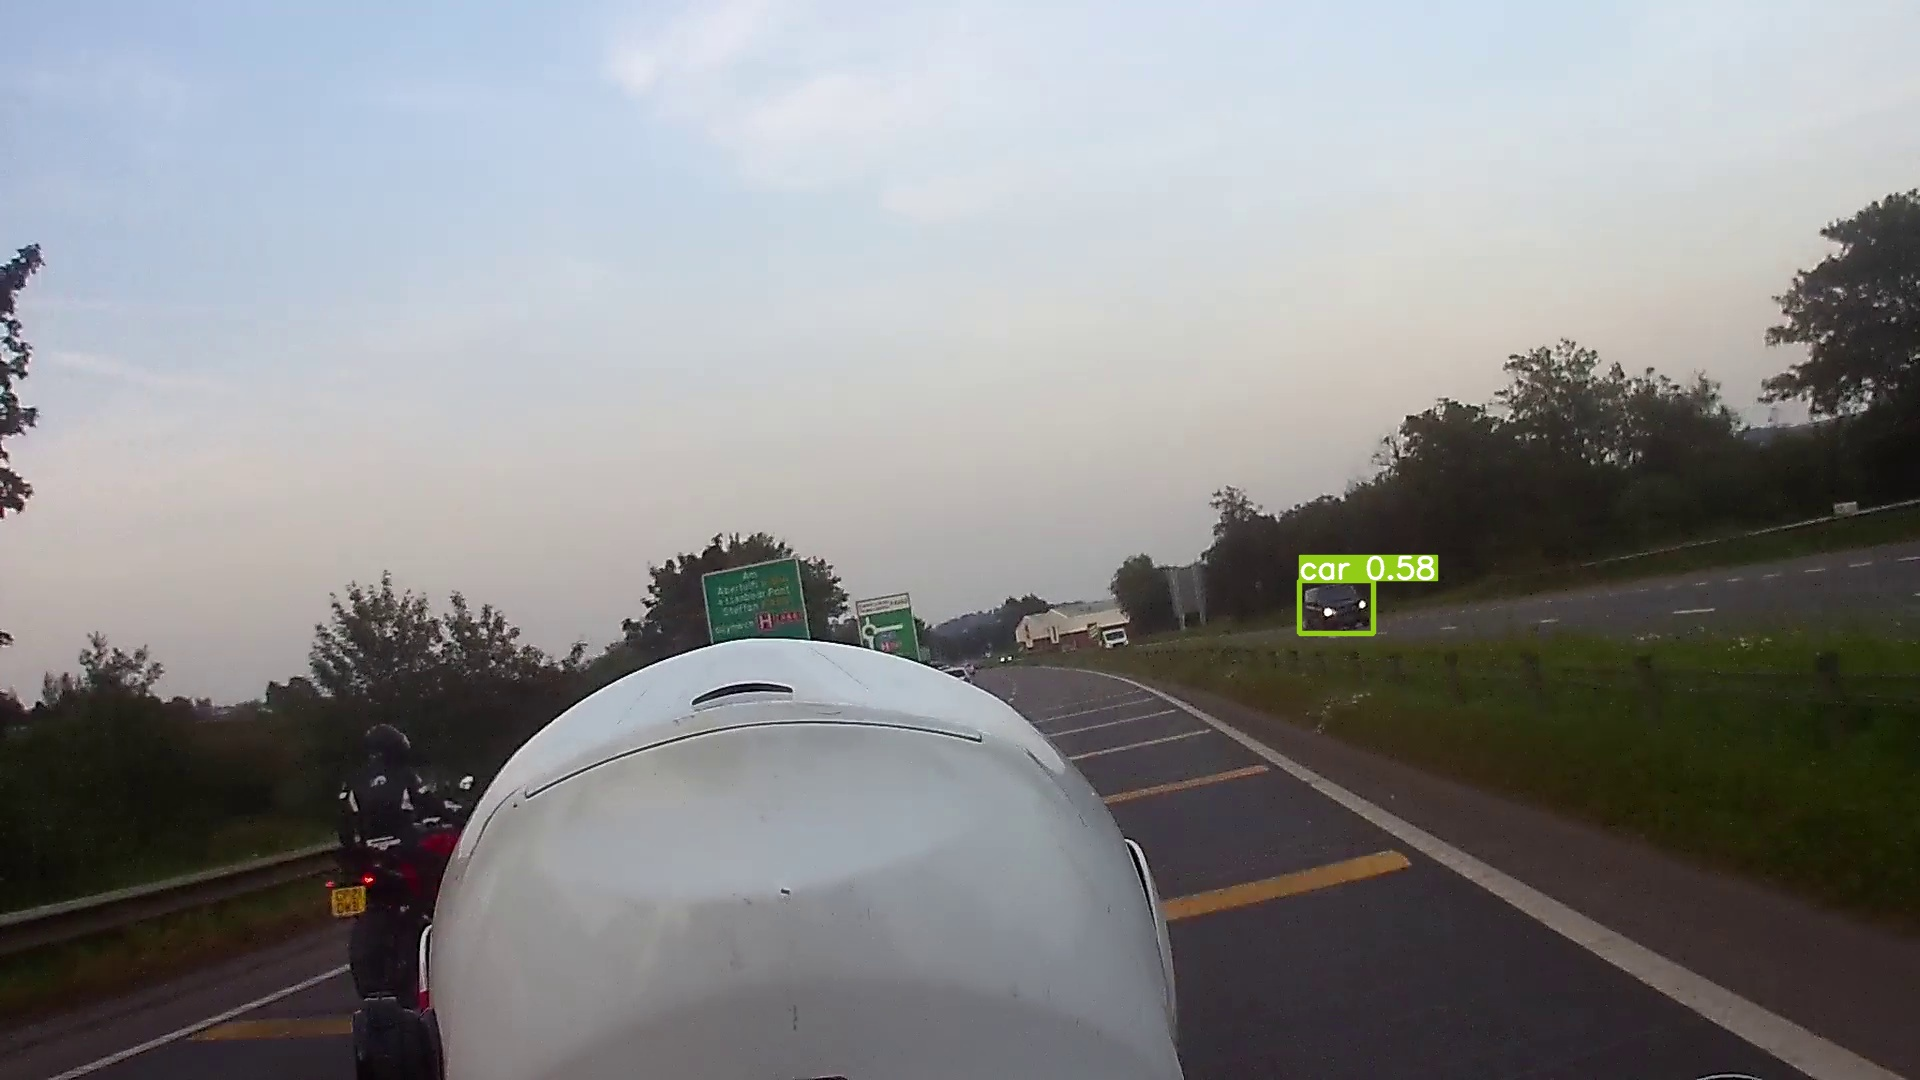
\includegraphics[width=1\linewidth]{Figures/scenarios/blindspot_day_t1/Misc_T4-342.jpg}
				}
				{
					\caption{Daytime Simulated Blindspot - Part 2}
					\label{fig:dtSimulatedBlindspotP2}
				}
			
				\ffigbox[1\linewidth]
				{
					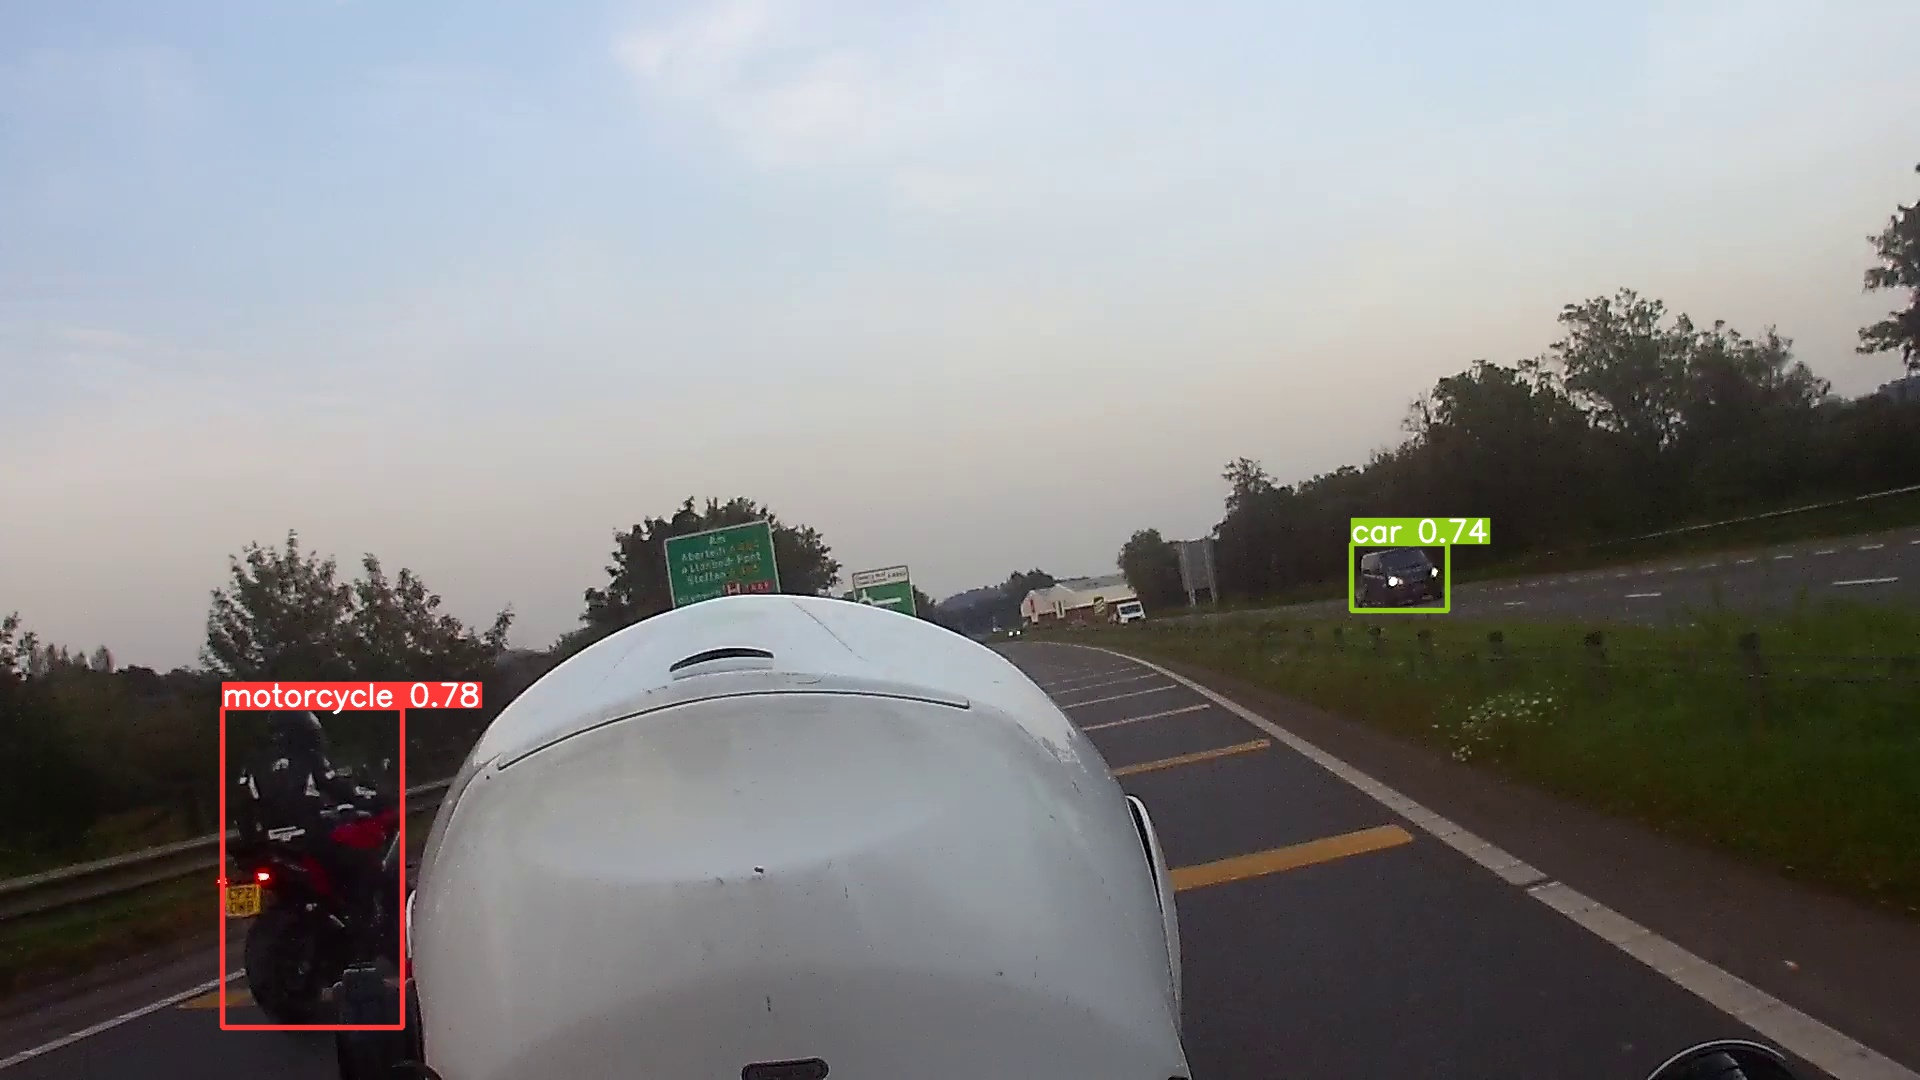
\includegraphics[width=1\linewidth]{Figures/scenarios/blindspot_day_t1/Misc_T4-349.jpg}
				}
				{
					\caption{Daytime Simulated Blindspot - Part 3}
					\label{fig:dtSimulatedBlindspotP3}
				}
			\end{floatrow}
		\end{figure}

		\clearpage
		Figures (\ref{fig:ntBlindspotP1},~\ref{fig:ntBlindspotP2},~\ref{fig:ntBlindspotP3}) showcases a overtake manoeuvre by a motorcyclist with the environment being dark. The results perform similarly to the previous example of a simulated daytime blindspot. However, it is important to take note that the `Dataset C' model has a poorer recognition accuracy. The first part shows the motorcycle just infront of the camera. This is described as a blindspot due to the lack of detection and visibility of the motorcycle. If a AV failed to recognise the motorcyclist prepared to overtake, then the AV may not adjust the speed in a safe manner. Successful classification of the motorcyclist with a 43\% uncertainty happened on the third scene.

		\begin{figure}[ht]
			\centering
			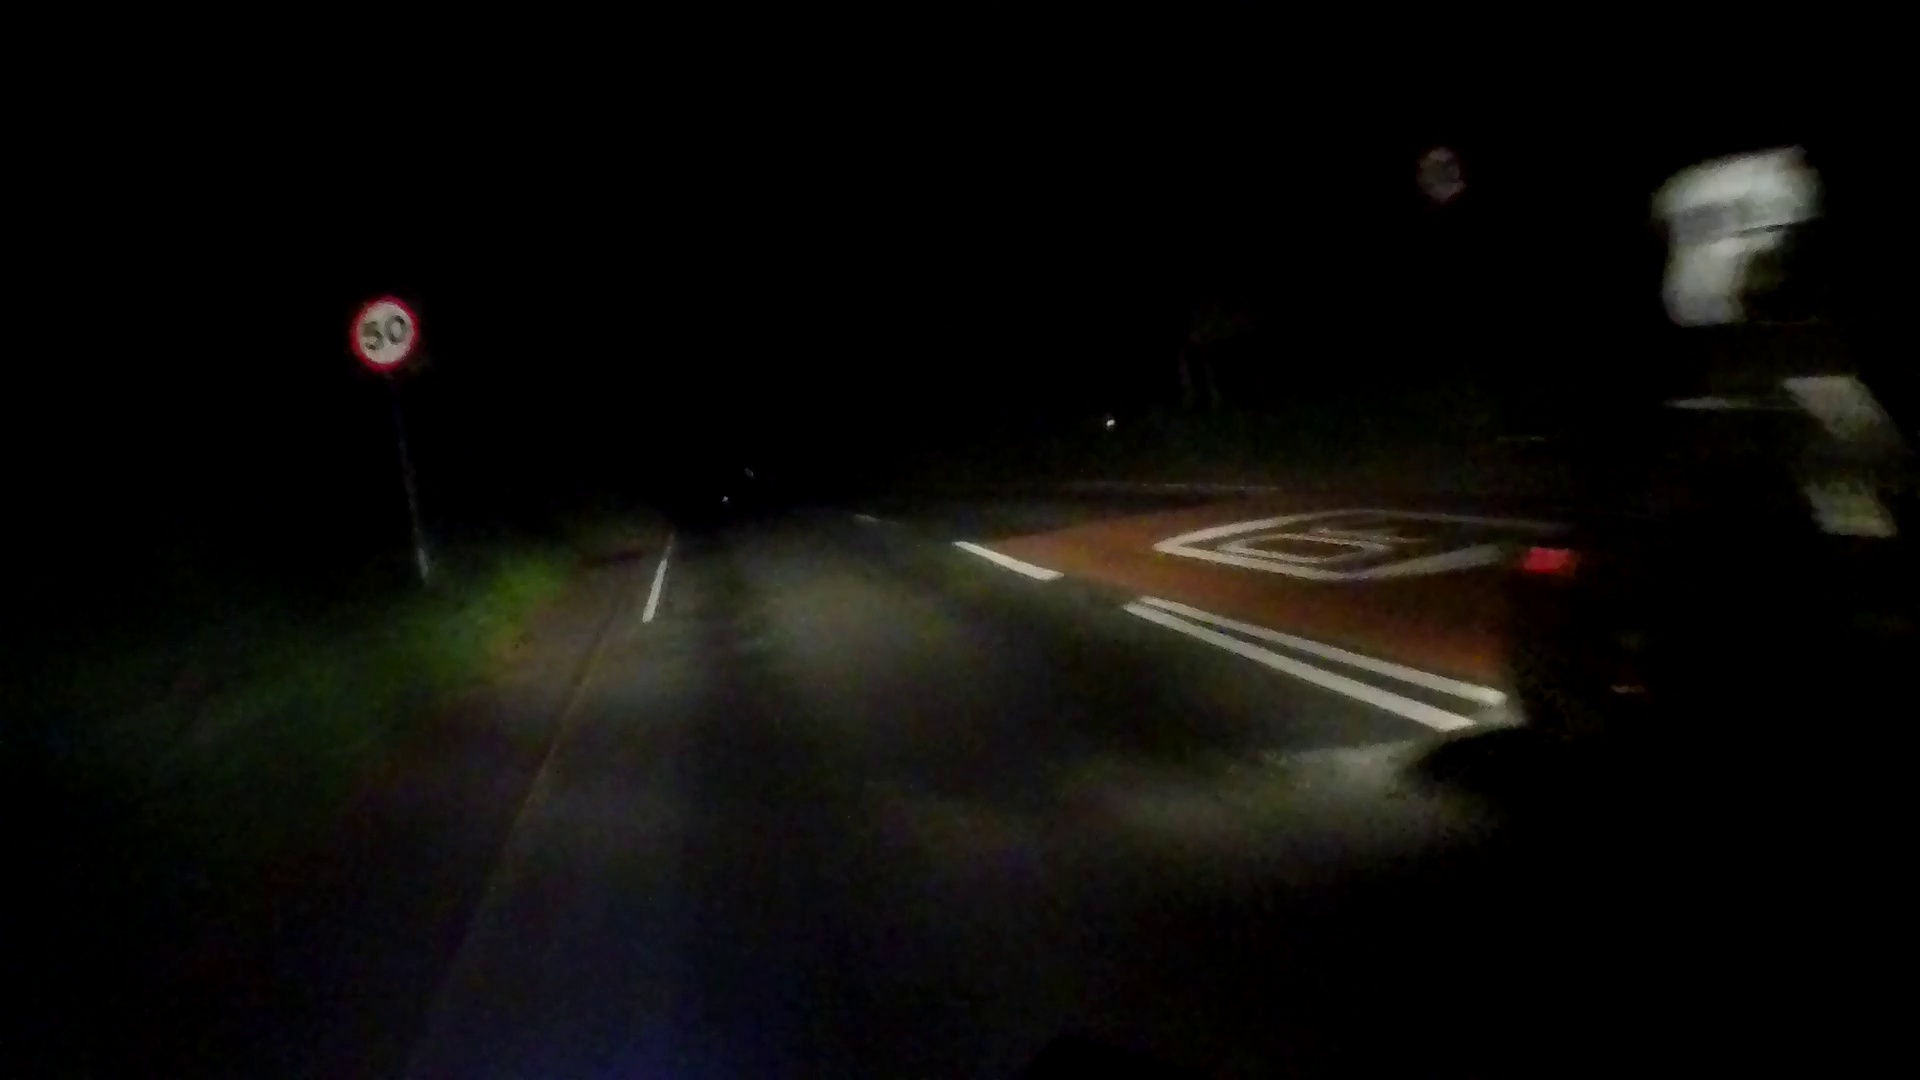
\includegraphics[width=.74\columnwidth]{Figures/scenarios/blindspot_night_t1/Night_BST1-191.jpg}
			\caption{Night-time Blindspot - Part 1}
			\label{fig:ntBlindspotP1}
		\end{figure}

		\begin{figure}[hb]
			\floatsetup{valign=t, heightadjust=object}
			\begin{floatrow}
				\ffigbox[1\linewidth]
				{
					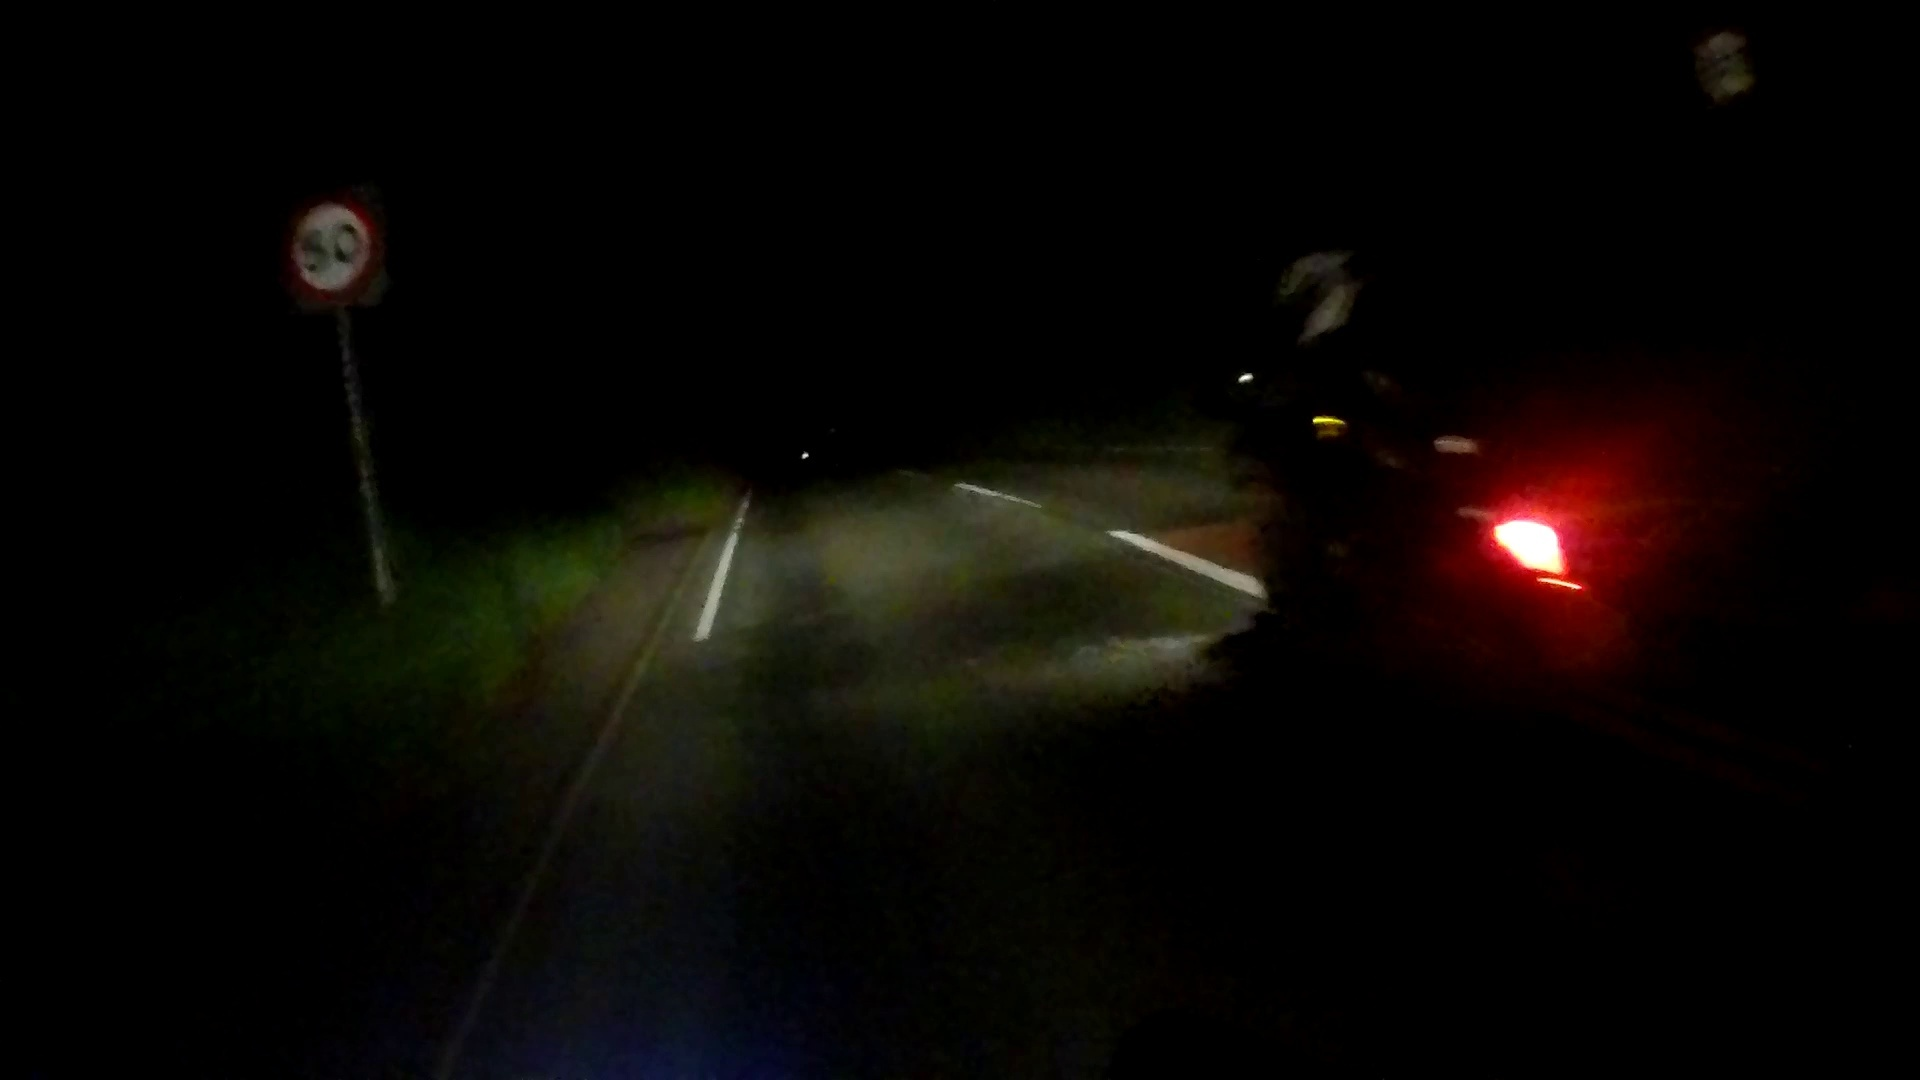
\includegraphics[width=1\linewidth]{Figures/scenarios/blindspot_night_t1/Night_BST1-202.jpg}
				}
				{
					\caption{Night-time Blindspot - Part 2}
					\label{fig:ntBlindspotP2}
				}
			
				\ffigbox[1\linewidth]
				{
					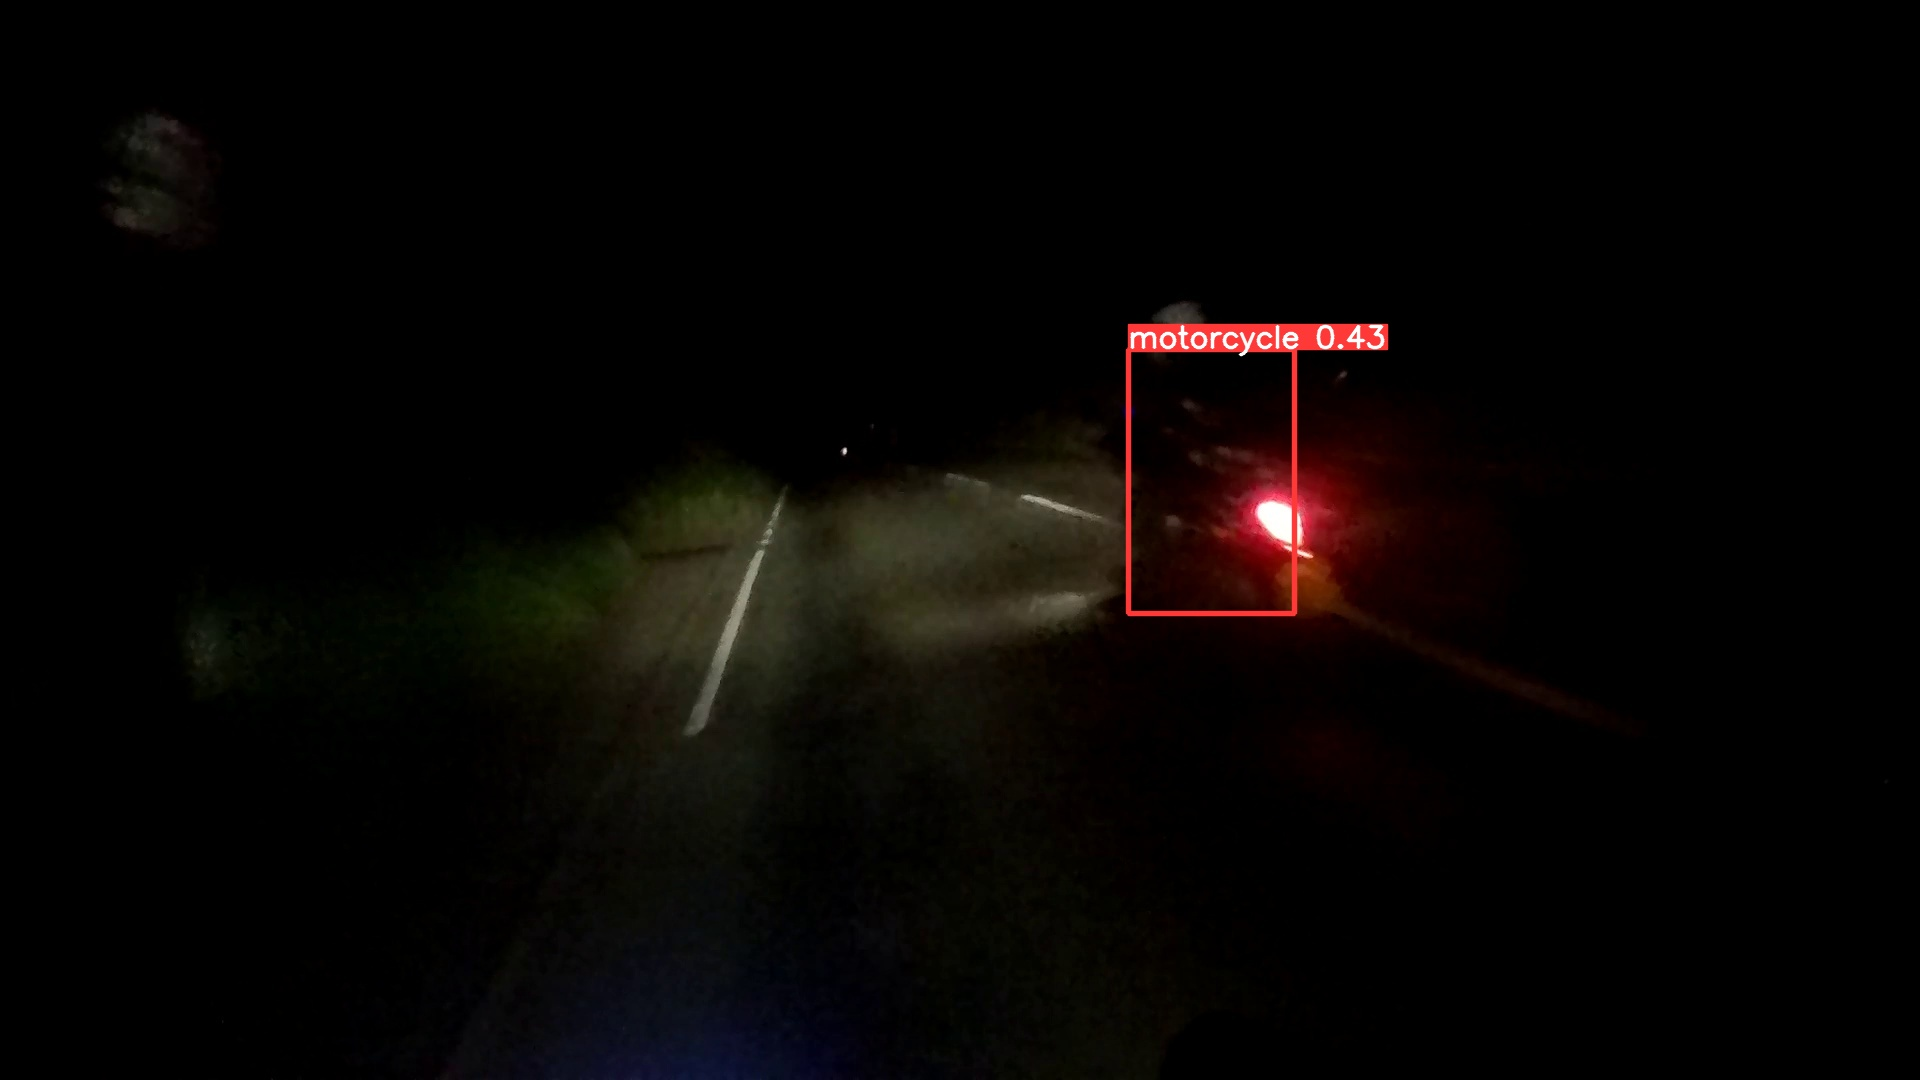
\includegraphics[width=1\linewidth]{Figures/scenarios/blindspot_night_t1/Night_BST1-211.jpg}
				}
				{
					\caption{Night-time Blindspot - Part 3}
					\label{fig:ntBlindspotP3}
				}
			\end{floatrow}
		\end{figure}

		\clearpage
		Figures (\ref{fig:ntReflectionP1},~\ref{fig:ntReflectionP2},~\ref{fig:ntReflectionP3}) demonstrate three scenarios involving on-coming vehicle lights, creating a `light' simulated blindspot. The motorcyclist is successfully detected in the first scenario, where the motorcyclist indicates to make a right turn. However, as a car approaches the motorcyclist, the camera fails to pick up the motorcyclist. The car flashed the motorcyclist to make the right turn, which, as the motorcyclist blocked the beam of the car, the motorcyclist was reidentified.
		\begin{figure}[ht]
			\centering
			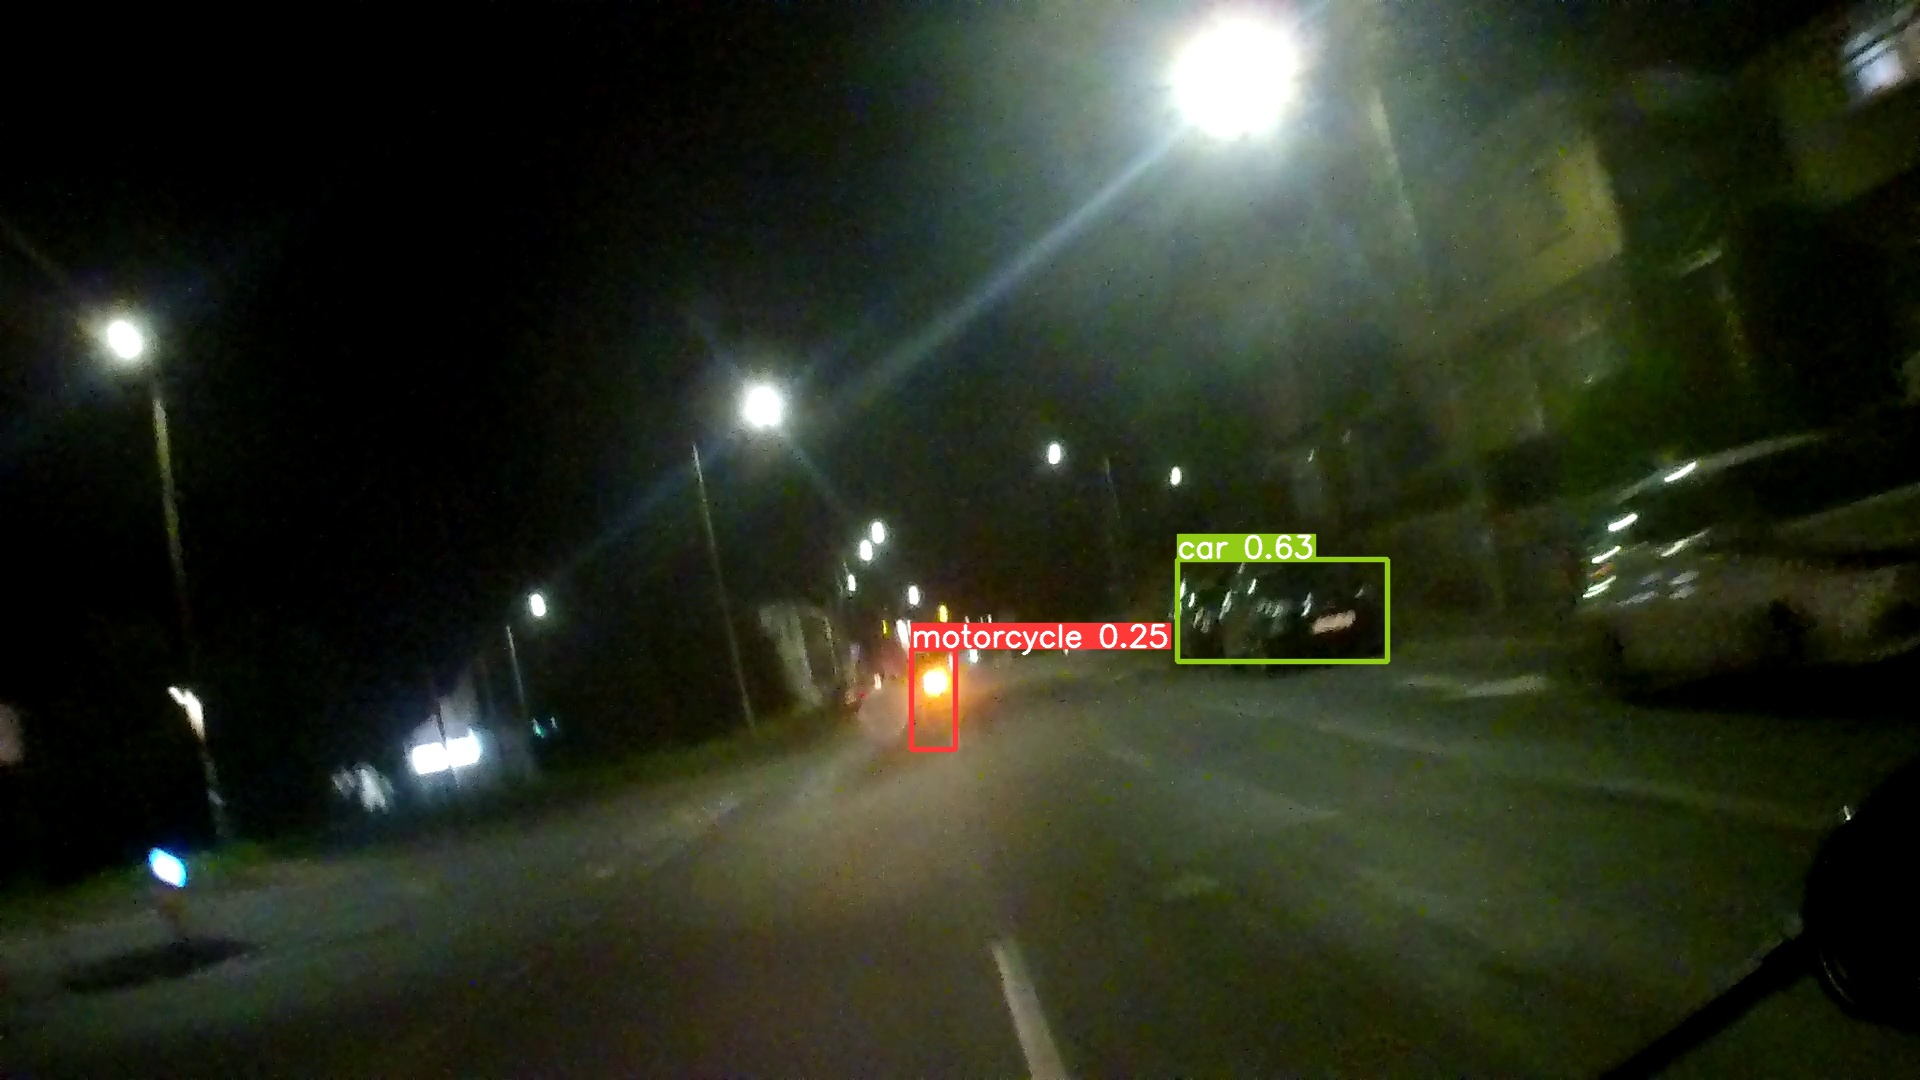
\includegraphics[width=.74\columnwidth]{Figures/scenarios/night_t1/Night_T1-505.jpg}
			\caption{Night-time Reflection - Part 1}
			\label{fig:ntReflectionP1}
		\end{figure}

		\begin{figure}[hb]
			\floatsetup{valign=t, heightadjust=object}
			\begin{floatrow}
				\ffigbox[1\linewidth]
				{
					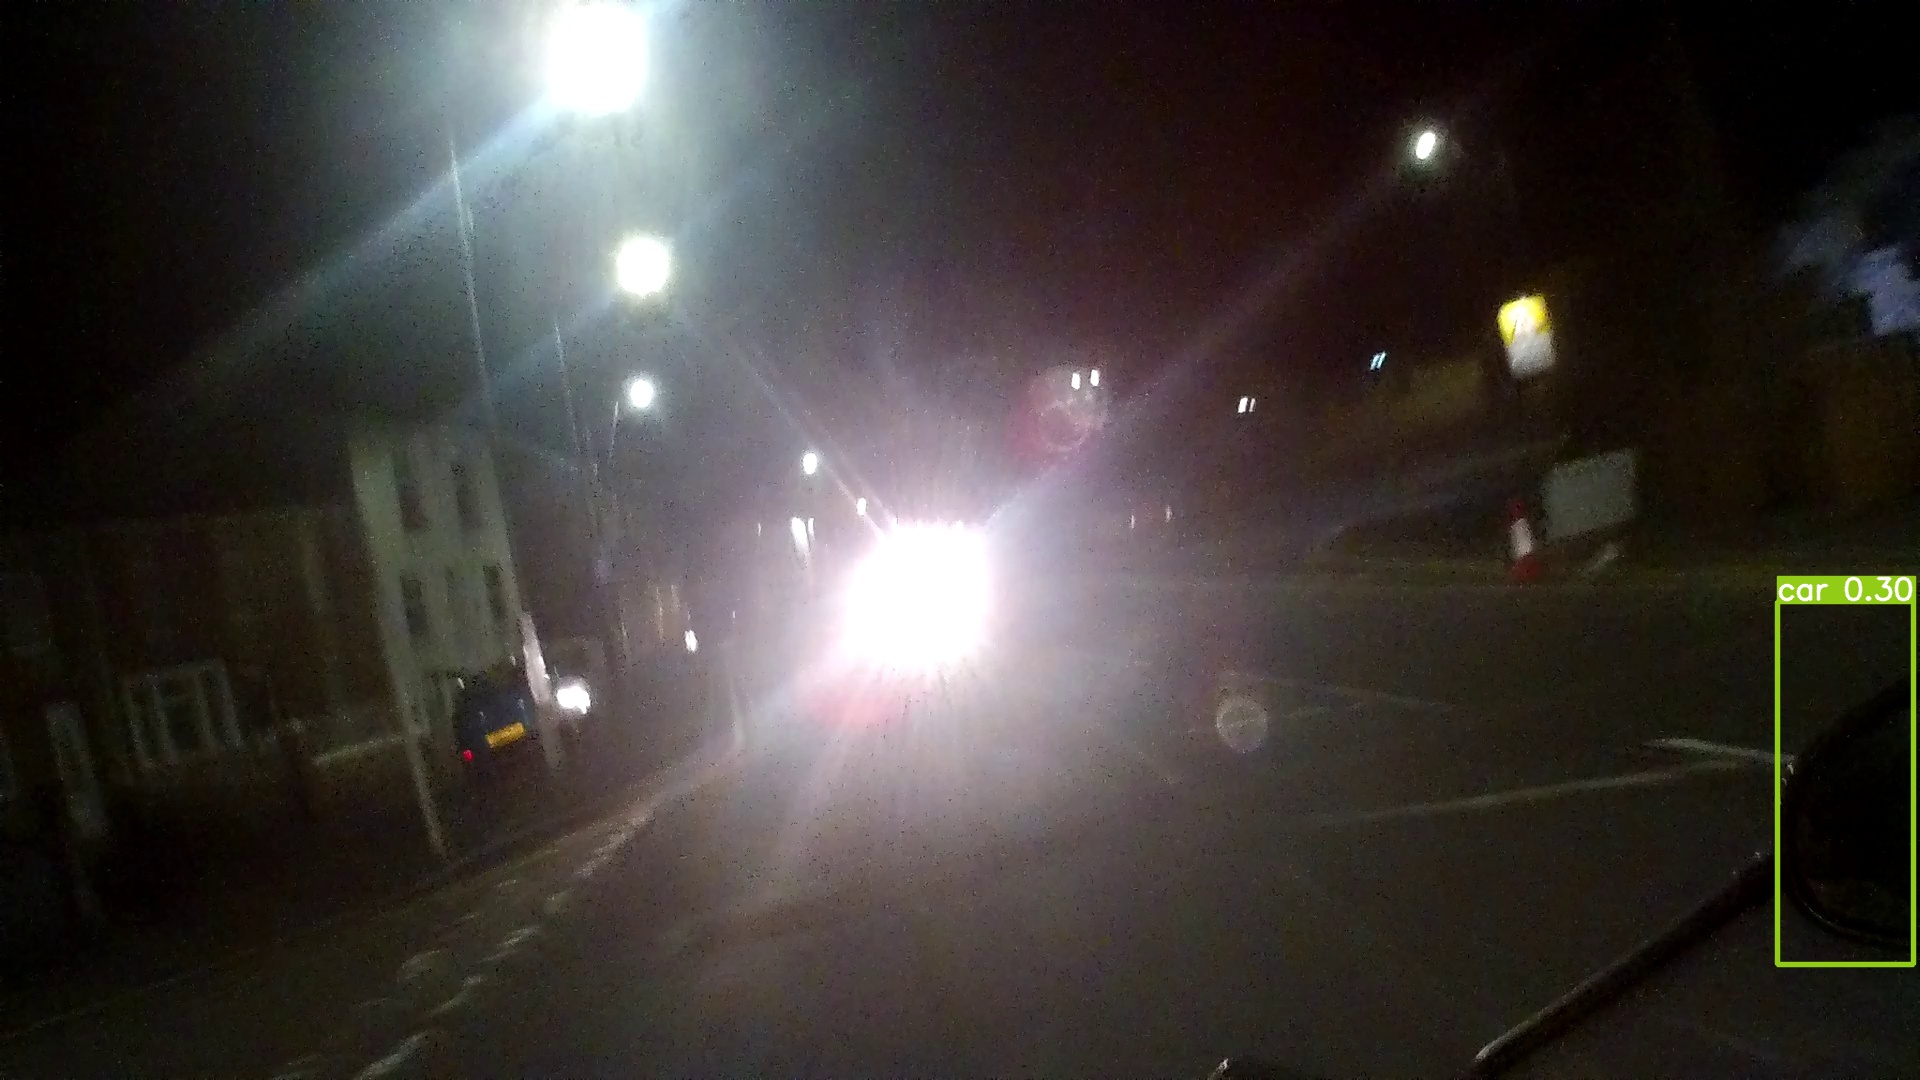
\includegraphics[width=1\linewidth]{Figures/scenarios/night_t1/Night_T1-526.jpg}
				}
				{
					\caption{Night-time Reflection - Part 2}
					\label{fig:ntReflectionP2}
				}
			
				\ffigbox[1\linewidth]
				{
					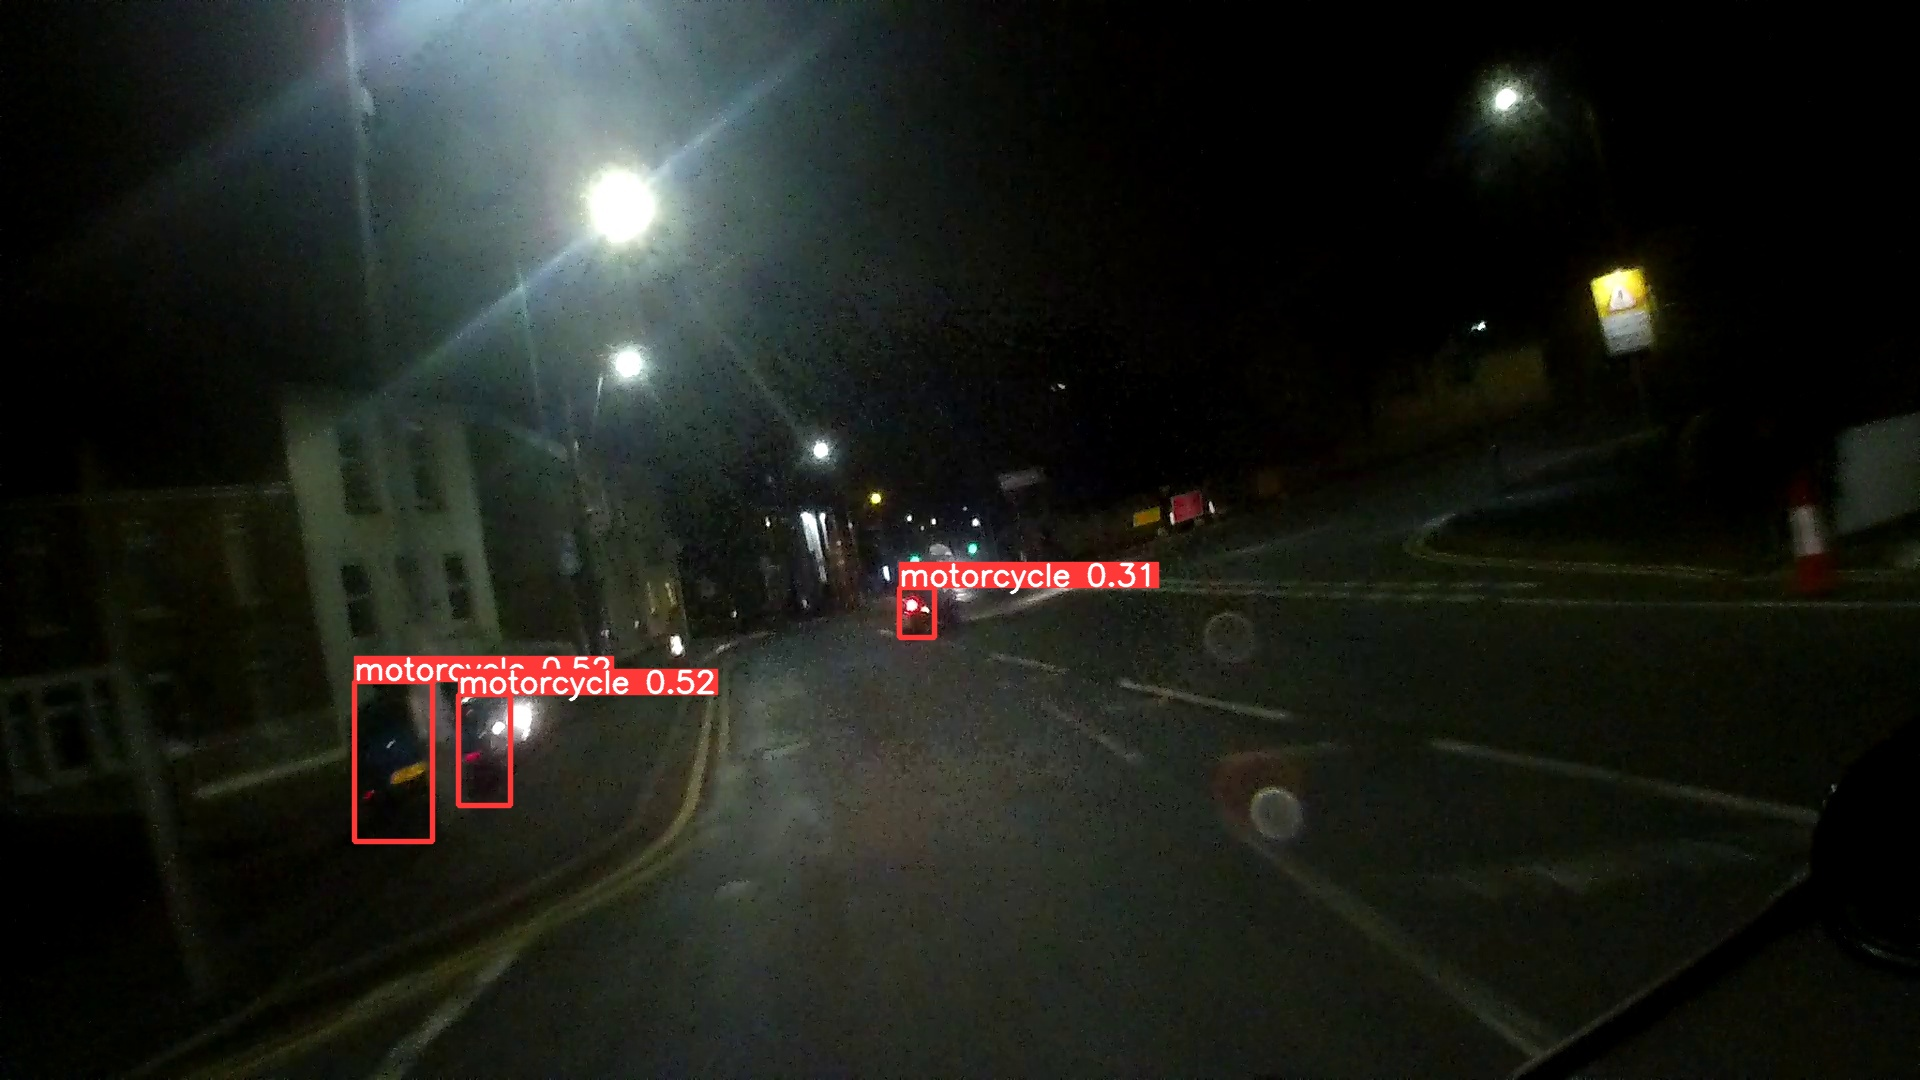
\includegraphics[width=1\linewidth]{Figures/scenarios/night_t1/Night_T1-529.jpg}
				}
				{
					\caption{Night-time Reflection - Part 3}
					\label{fig:ntReflectionP3}
				}
			\end{floatrow}
		\end{figure}

\chapter{Dicussion}
\label{chap:discussion}
	\section{Training Sequence}
		The trained classification uses Asian and US footage to train the model. According to the classification models found in figures (\ref{fig:ukDatasetYolov5LargeWeight},~\ref{fig:mtpDatasetYolov5LargeWeight}), the motorcycle had an 81\% accuracy within fig~\ref{fig:ukDatasetYolov5LargeWeight}, with 39\% outliers identifying motorcycle objects as Scooters, with a minimal of 15\% outliers identifying as background. In comparison to the Motorcycle, Trike and Person model, found in fig~\ref{fig:mtpDatasetYolov5LargeWeight}, the motorcycle had a 77\% accuracy, with 32\% of outliers identifying as background.

		Figures (\ref{fig:ukDatasetYolov5LargeWeightPRCurve},~\ref{fig:mtpDatasetYolov5LargeWeightPRCurve}) show the Precision and Recall curves plotted on a graph, giving information on any performance issues with the training models. The PR curves for both models demonstrate high precision across varying levels of recall, indicative of robust performance. Although, figure~\ref{fig:ukDatasetYolov5LargeWeightPRCurve} appears to have a higher precision for the longer part of the training process, compared to figure~\ref{fig:mtpDatasetYolov5LargeWeightPRCurve}. The worse performers of the model are scooters, vans, person and minivans in precision and perform well when it comes to recall. In comparison, figure~\ref{fig:mtpDatasetYolov5LargeWeightPRCurve} shows a similar illustration. According to the key of figure~\ref{fig:ukDatasetYolov5LargeWeightPRCurve}, motorcycles had a higher precision peak at 77.5\% compared to figure~\ref{fig:mtpDatasetYolov5LargeWeightPRCurve}. The model architecture performs well when training the given dataset scenarios. Perhaps larger weights could increase the precision and recall curve during training. It is worth mentioning that the preparation of the datasets functions well during the training process, and no underlying problems are showing, especially for motorcycle data.

		Figure~\ref{fig:ntDatasetYolov5MediumWeight} displays the confusion matrix of the fake night-time training to see if the quality of the results would increase. The model has a lower detection percentage, with a 67\% accuracy of picking up a motorcycle. However, the model should have a higher accuracy of night-time detection, whereas the other datasets may struggle. This model is unoptimised for day-time scenarios and gives us an understanding of any issues that may occur at night-time when LiDAR sensors are indispensable compared to vision alone. This dataset lowered the accuracy down to the visibility levels, and motorcycles are hard to see in general, down to the reduced size and light systems. An ideal solution to this problem, is having real night footage of motorcycles, mixed with other vehicles, and applying contrast, embevels and other image filters to make the outlines stand out. Although, in this practical sense, the datasets needed to be modified to symbolise a dark feel to see if this would help detection rate for night-time use. The model overall achieves good results and is suitable to carry out theoretical experiments.

		During the testing sequence, the larger trained model was selected. Arguably, the 81\% accuracy for motorcycles, with 39\% outliers identifying as scooters or even a 3\% as a trike, is still safer than having most motorcycles identified as background objects. The accuracy of this training may come under a few situations, including better object classification training material for motorcycles, especially in foggy, wet, overtaking and filtering situations within the UK.

	\section{Testing Sequence}
		A few issues come to light after running through the gathered test results. The footage involves mixed scenarios, including wet, dry and overtaking procedures. There are a few prospects that need addressing when observing the test footage. Before going into a deeper level of understanding why accurate classifications are essential, and it does not stop at detecting a motorcycle, as hand gestures and a person's body are equally important when it comes to indicating, warning they are braking, or if a fortunate accident were to happen, including a pillion (passenger of the vehicle) or operator was to come off in the road suddenly. A critical emphasis would include whether the AV would detect this or only register the motorcycle still riding in a straight line, causing the AV not to stop, avoiding potential death.

	\subsection*{Hypothesis A - Blindspots and Reaction Time}
		Figures (\ref{fig:detectionOfOneMotorcycle}~\ref{fig:lateClassificationP1}~\ref{fig:lateClassificationP2}) display the importance of safety when rolling out AVs within the UK. The detection of motorcycles seems to be limited. However, with some tracking implementation, when detection is detected, it could help the process. Although, tracking does not guarantee that the motorcycles are always in sight. A common theme found when performing these detections is that detection was useless when a motorcycle started to be further in the distance. This finding leads to figure~\ref{fig:lateClassificationP1} and~\ref{fig:lateClassificationP2} where the on-coming motorcycle was not immediately detected, and if for some reason the AV had to make a right turn or a swerve to the right, rather than applying the braking system, then the misfortunate rider would have zero to no time to react the intention of the AV.

		Figures (\ref{fig:dtSimulatedBlindspotP1},~\ref{fig:dtSimulatedBlindspotP2},~\ref{fig:dtSimulatedBlindspotP3}) use a Pillion to generate a blindspot scenario to test out the theory. A vehicle will have a clear view based on where the cameras are mounted. Although that vehicle will have designated blindspot locations when a motorcycle passes, this method is meant to restrict the picture to the road to test side views. The experiment works as expected, and during the first figure~\ref{fig:dtSimulatedBlindspotP1}, the motorcyclist is on camera, although, perhaps with the darkness of the rider, the model fails to classify the motorcycle. During the second figure~\ref{fig:dtSimulatedBlindspotP2}, the motorcyclist is still undetected, and during each frame, the motorcyclist has been braking. This scenario is considered dangerous if the motorcyclist were to move to the right lane by dangerously overtaking, or if a situation in front had happened, the AV may not identify this situation and cause a potential collision.

		Figures (\ref{fig:ntBlindspotP1},~\ref{fig:ntBlindspotP2},~\ref{fig:ntBlindspotP3}) identifies the dangers of motorcyclists at night. Motorcyclists are hard to see at night. However, human intelligence can detect motorcyclists by noticing headlights in rearview mirrors. However, when a motorcyclist overtakes, the motorcyclist knows that the human driver can identify the motorcyclist's bright clothing, reflective areas on the helmet, or front headlights, giving them a sense of security that the driver will slow and acknowledge the motorcyclist to continue a safe overtake. However, in the scenarios showcased, the model fails to identify the motorcycle on the initial passing, and it also fails to acknowledge the motorcyclist when it moves into a lane. This observation could explain the issues AV manufacturers started seeing when LiDAR was removed.

	\subsection*{Hypothesis B - Low Visibility Conditions}
		Figures (\ref{fig:ntReflectionP1},~\ref{fig:ntReflectionP2},~\ref{fig:ntReflectionP3}) indicate a potential camera issue that the AV policies must not overlook. The motorcyclist indicating to turn right is correctly identified in fig~\ref{fig:ntReflectionP1} before any vehicle appears. When a car approaches, the car flashes the motorcyclist out. However, the camera loses all vision of the motorcyclist. The motorcyclist is reclassified when they make the turn. However, as mentioned in the findings, the big problem is that when the camera loses vision due to reflection of the oncoming vehicle, would the AV pick up speed to 30MPH, not realising the motorcyclist has not yet made a move? Another situation could include that the motorcyclist never made the turn and stopped, awaiting the car to pass. Would the AV continue and ram the motorcyclist?


	\subsection*{Hypothesis C - Poor Weather Conditions}
		In figures (\ref{fig:detectionOfMotorcycleW1},~\ref{fig:detectionOfMotorcycleW2},~\ref{fig:detectionOfMotorcycleW3}) display three scenarios. The evident problem is that the camera used kept getting water on, so the camera used in AVs must have the resilience to repel water to remain safe on the road. However, the camera fails to pick up the motorcycle in figure~\ref{fig:detectionOfMotorcycleW3}, noting that not all motorcycles may have their lights on. In this case, the light is on. However, fog lights were not required, so even having any implementation on the vehicle would not help, as it was not the right condition for the given scenario and could cause blindness and eye fatigue to other road users.

\chapter{Reflection}
\label{chap:reflection}
	After reviewing the findings and discussion referring to blindspots, it was found that motorcycle detection struggled when the vehicle was distant or had poor visibility. Motorcyclists had the potential of poor recognition, causing a visible blindspot scenario, and still have the potential to hide in AV camera blind spots. This fact meant that no matter the technology that the self-driving vehicle adopted, it was not a hundred percent that the motorcycle was recognised. This poor indication could impact the AV's reaction time, or the AV may not even react if any scenarios within the findings played out. 
		
	After observing the situation, ADAS systems will help provide research on this impact. However, it means that drivers will have to pay close attention to their surroundings and cannot get complacent as motorcycles can filter within the UK and are getting more popular on the UK roads. Relying solely on the current models and camera equipment may not fully account for blindspots. It may reduce the AV or even driver reaction time as motorcycles are already hard to see by drivers thoroughly in charge of the vehicle.

	The findings and discussion show concern for when a motorcyclist was in the distance or when the motorcycle was riding at night. The classification was late, and this means that the AV may not be able to recognise an issue to counter-move. Also, a scenario where LiDAR would have been helpful was when a car's headlights caused glare to the camera, which hid the motorcycle that was turning right. This fact meant the AV could continue driving forward, killing the motorcyclist as the motorcyclist was hidden with glare, where human intelligence would have still seen the motorcyclist clear as day, slowing down.

	Hypothesis A: `Motorcycles have blindspots often overlooked by human drivers, which AVs can detect and avoid.' This statement is true. AVs can detect and avoid motorcycle dangers. However, this is under the impression that the driver is in control most of the time. Suppose a self-driving car had full access to the vehicle most of the time. In that case, this statement is misleading, as the vehicle will most likely have a slight chance of detecting every motorcyclist on the road or reacting wrongly when a motorcyclist reacts. This described scenario is due to the motorcyclist training involved. Riders are continuously trained to analyse and react, so a rider has accessed their mistake and has an idea to react. In contrast, the AV may have a similar idea to preserve itself, causing both vehicles to block each other, causing a deadly fatality. This issue is another reason why research must be prioritised across many organisations to get awareness. 

	Hypothesis B: `In low light conditions, AVs may struggle to accurately detect and identify motorcycles, leading to potential safety issues on the road.' This statement appears to be true. However, not in the sense of low light conditions, as the model did exceptionally well to detect the motorcyclist after potential blindspot areas. Although more of an unconventional stance of light glare on the camera. With further editing, the glare could be reduced and solving this issue. However, from the experiments, the object classification struggles when glare appears.

	Hypothesis C: `Poor weather conditions, such as heavy rain or poor visibility, can make it difficult for AVs to detect and react to motorcycles, increasing the risk of accidents.' This statement is proven to be valid from the experiments. Camera glare, water droplets, and spray influence this fact. Even if the AV camera technology can repel water, the statement stands true, as the vehicle spray makes it very hard to see, affecting the classification side. 

	It is questionable whether LiDAR could help classify the motorcyclist better and that the issues AV manufacturers were suffering with still needed to be ironed out and furthered in development. Rather than abandoning the technology's early stages, which could ultimately save a motorcyclist's life.

\chapter*{Terminology}
List of terminologies used in this document:-
\begin{itemize}
	\item ADS - Advanced Driving System. 
	\item ADAS - Advanced Driver-Assistance System.
	\item ASDE - Autonomous System Design Entity.
	\item ATB - Approved Trained Body.
	\item AV - Autonomous Vehicles.
	\item CBT - Compulsory Basic Training.
	\item CI - Continuous Integration.
	\item DSA - Driving Standards Agency.
	\item HSS - Hybrid State System.
	\item HMM - Hidden Markov Models.
	\item KFM - Kalman Filter Models.
	\item MOT - Ministry of Transport.
	\item NHS - National Health Services.
	\item NUIC - No-User-In-Charge.
	\item RAD - Rapid Application Development.
	\item TDD - Test-Driven Development.
	\item UIC - User-In-Charge
	\item VCA - Vehicle Certification Authority.
	\item YOLO - You Only Look Once.
\end{itemize}
  

%----------
%	Bibliography
%----------	

\clearpage
\nocite{*}
\small{\bibliographystyle{IEEEtran}
	\bibliography{ref}}

%----------
%	Appendix
%----------	

% If your work includes Appendix, you can uncomment the following lines
%\chapter* {Appendix x}
%\pagenumbering{gobble} % Appendix pages are not numbered

\end{document}